% !TeX program = lualatex
% ALIUS Bulletin native visual reconstruction source.
% Generated from off-repo reference layout data; does not include or input a pre-existing article PDF.
\ifdefined\ALIUSIssueBuild
\else
\documentclass{article}
\usepackage[paperwidth=595.0000bp,paperheight=842.0000bp,margin=0bp]{geometry}
\usepackage{graphicx}
\usepackage{xcolor}
\usepackage{tikz}
\usepackage{iftex}
\usepackage[hidelinks]{hyperref}
\ifPDFTeX
  \usepackage[T1]{fontenc}
  \usepackage[utf8]{inputenc}
  \usepackage{textcomp}
  \usepackage{amssymb}
\else
  \usepackage{fontspec}
\fi
\pagestyle{empty}
\fi
\ifPDFTeX
  \providecommand{\ALIUSDeclareUnicodeFallbacks}{%
    \DeclareUnicodeCharacter{00AC}{\ensuremath{\neg}}%
    \DeclareUnicodeCharacter{00BE}{\ensuremath{\frac{3}{4}}}%
    \DeclareUnicodeCharacter{0101}{\=a}%
    \DeclareUnicodeCharacter{0107}{\'c}%
    \DeclareUnicodeCharacter{012B}{\=\i}%
    \DeclareUnicodeCharacter{0131}{\i}%
    \DeclareUnicodeCharacter{0142}{\l}%
    \DeclareUnicodeCharacter{015B}{\'s}%
    \DeclareUnicodeCharacter{016B}{\=u}%
    \DeclareUnicodeCharacter{025C}{q}%
    \DeclareUnicodeCharacter{0278}{t}%
    \DeclareUnicodeCharacter{02AE}{Th}%
    \DeclareUnicodeCharacter{02B0}{ff}%
    \DeclareUnicodeCharacter{02B4}{ffi}%
    \DeclareUnicodeCharacter{02BE}{ft}%
    \DeclareUnicodeCharacter{02BF}{fi}%
    \DeclareUnicodeCharacter{02C0}{fl}%
    \DeclareUnicodeCharacter{02C1}{fi}%
    \DeclareUnicodeCharacter{02D9}{Th}%
    \DeclareUnicodeCharacter{02EF}{gy}%
    \DeclareUnicodeCharacter{0394}{\ensuremath{\Delta}}%
    \DeclareUnicodeCharacter{03B2}{\ensuremath{\beta}}%
    \DeclareUnicodeCharacter{03BA}{\ensuremath{\kappa}}%
    \DeclareUnicodeCharacter{068D}{-}%
    \DeclareUnicodeCharacter{08BC}{ti}%
    \DeclareUnicodeCharacter{099E}{ti}%
    \DeclareUnicodeCharacter{1E43}{\d{m}}%
    \DeclareUnicodeCharacter{1E47}{\d{n}}%
    \DeclareUnicodeCharacter{1E63}{\d{s}}%
    \DeclareUnicodeCharacter{201C}{``}%
    \DeclareUnicodeCharacter{201D}{''}%
    \DeclareUnicodeCharacter{2260}{\ensuremath{\neq}}%
    \DeclareUnicodeCharacter{25A1}{\ensuremath{\square}}%
  }%
  \ifdefined\ALIUSIssueBuild\else\ALIUSDeclareUnicodeFallbacks\fi
  \providecommand{\ALIUSFontLatoLight}{\fontfamily{lato-LF}\fontseries{l}\selectfont}
  \providecommand{\ALIUSFontLatoRegular}{\fontfamily{lato-LF}\fontseries{m}\selectfont}
  \providecommand{\ALIUSFontLatoItalic}{\fontfamily{lato-LF}\fontseries{m}\itshape}
  \providecommand{\ALIUSFontLatoLightItalic}{\fontfamily{lato-LF}\fontseries{l}\itshape}
  \providecommand{\ALIUSFontCormorantRegular}{\fontfamily{CormorantGaramond-LF}\fontseries{m}\selectfont}
  \providecommand{\ALIUSFontCormorantLight}{\fontfamily{CormorantGaramond-LF}\fontseries{l}\selectfont}
  \providecommand{\ALIUSFontCormorantMedium}{\fontfamily{CormorantGaramond-LF}\fontseries{medium}\selectfont}
  \providecommand{\ALIUSFontCormorantBold}{\fontfamily{CormorantGaramond-LF}\fontseries{b}\selectfont}
  \providecommand{\ALIUSFontCormorantItalic}{\fontfamily{CormorantGaramond-LF}\fontseries{m}\itshape}
  \providecommand{\ALIUSFontTimes}{\fontfamily{ptm}\selectfont}
  \providecommand{\ALIUSFontCalibri}{\fontfamily{phv}\selectfont}
  \providecommand{\ALIUSFontCambria}{\fontfamily{ptm}\selectfont}
  \providecommand{\ALIUSFontSymbolFallback}{\fontfamily{ptm}\selectfont}
\else
  \providecommand{\ALIUSFontLatoLight}{\fontspec{Lato Light}}
  \providecommand{\ALIUSFontLatoRegular}{\fontspec{Lato Regular}}
  \providecommand{\ALIUSFontLatoItalic}{\fontspec{Lato Italic}}
  \providecommand{\ALIUSFontLatoLightItalic}{\fontspec{Lato Light Italic}}
  \providecommand{\ALIUSFontCormorantRegular}{\fontspec{Cormorant Garamond Regular}}
  \providecommand{\ALIUSFontCormorantLight}{\fontspec{Cormorant Garamond Light}}
  \providecommand{\ALIUSFontCormorantMedium}{\fontspec{Cormorant Garamond Medium}}
  \providecommand{\ALIUSFontCormorantBold}{\fontspec{Cormorant Garamond Bold}}
  \providecommand{\ALIUSFontCormorantItalic}{\fontspec{Cormorant Garamond Italic}}
  \providecommand{\ALIUSFontTimes}{\fontspec{Times New Roman}}
  \providecommand{\ALIUSFontCalibri}{\fontspec{Calibri}}
  \providecommand{\ALIUSFontCambria}{\fontspec{Cambria}}
  \providecommand{\ALIUSFontSymbolFallback}{\fontspec{Times New Roman}}
\fi
\providecommand{\ALIUSPullQuoteOpen}{\textquotedblleft}
\providecommand{\ALIUSPullQuoteClose}{\textquotedblright}
\providecommand{\ALIUSPullQuoteBlockAt}[4]{%
  \node[anchor=north west,inner sep=0pt,outer sep=0pt,xshift=12bp,text=ALIUSC595959,font=\ALIUSFontLatoLight\fontsize{15.000bp}{18.000bp}\selectfont\hyphenpenalty10000\exhyphenpenalty10000\relax] (ALIUSPullQuoteBody) at (#1bp,-#2bp) {\begin{tabular}{@{}c@{}}#4\end{tabular}};%
  \node[anchor=north east,inner sep=0pt,outer sep=0pt,text=ALIUSC7F7F7F,xshift=-6bp] at (ALIUSPullQuoteBody.north west) {%
    {\ALIUSFontCormorantLight\fontsize{32.000bp}{32.000bp}\selectfont\ALIUSPullQuoteOpen}%
  };%
  \node[anchor=south west,inner sep=0pt,outer sep=0pt,text=ALIUSC7F7F7F,xshift=6bp,yshift=-7bp] at (ALIUSPullQuoteBody.south east) {%
    {\ALIUSFontCormorantLight\fontsize{32.000bp}{32.000bp}\selectfont\ALIUSPullQuoteClose}%
  };%
}
\providecommand{\ALIUSNotableQuoteAt}[4]{%
  \ALIUSPullQuoteBlockAt{#1}{#2}{#3}{#4}%
}
\providecommand{\ALIUSMaybeNotableQuoteAt}[4]{%
  \if\relax\detokenize{#4}\relax\else\ALIUSNotableQuoteAt{#1}{#2}{#3}{#4}\fi%
}
\providecommand{\ALIUSRefAnchor}[1]{\hypertarget{#1}{}}
\providecommand{\ALIUSCitationLink}[2]{\hyperlink{#1}{#2}}
\definecolor{ALIUSC000000}{HTML}{000000}
\definecolor{ALIUSC0563C1}{HTML}{0563C1}
\definecolor{ALIUSC1A1718}{HTML}{1A1718}
\definecolor{ALIUSC1F8135}{HTML}{1F8135}
\definecolor{ALIUSC595959}{HTML}{595959}
\definecolor{ALIUSC767171}{HTML}{767171}
\definecolor{ALIUSC7F7F7F}{HTML}{7F7F7F}
\definecolor{ALIUSCBFBFBF}{HTML}{BFBFBF}
\providecommand{\ALIUSPlacedText}[6]{%
  \node[anchor=north west,inner sep=0pt,outer sep=0pt,text=#4] at (#1bp,-#2bp) {%
    \resizebox{#3bp}{!}{{#5\fontsize{#6bp}{#6bp}\selectfont #6\kern0pt}}%
  };%
}
\providecommand{\ALIUSPlacedTextContent}[7]{%
  \node[anchor=north west,inner sep=0pt,outer sep=0pt,text=#4] at (#1bp,-#2bp) {%
    \resizebox{#3bp}{!}{{#5\fontsize{#6bp}{#6bp}\selectfont #7}}%
  };%
}
% --- Draft abstract retained as comments; not rendered in reconstruction. ---
% \section*{Abstract}
% [TBA]\par
% --- End draft abstract. ---
\ifdefined\ALIUSIssueBuild
\else
\begin{document}
\fi
% Page 1
\thispagestyle{empty}
\noindent\begin{tikzpicture}[remember picture,overlay,x=1bp,y=1bp,shift={(current page.north west)}]
  \fill[ALIUSC767171] (69.640bp,-787.000bp) rectangle ++(456.480bp,-0.720bp);
  \fill[ALIUSC1F8135] (352.840bp,-187.480bp) rectangle ++(91.440bp,-0.240bp);
  \fill[ALIUSC1F8135] (352.840bp,-259.480bp) rectangle ++(86.400bp,-0.240bp);
  \fill[ALIUSC1F8135] (352.840bp,-317.080bp) rectangle ++(140.160bp,-0.240bp);
  \fill[ALIUSCBFBFBF] (347.320bp,-158.200bp) rectangle ++(0.240bp,-135.840bp);
  \fill[ALIUSCBFBFBF] (347.320bp,-294.040bp) rectangle ++(0.240bp,-2.160bp);
  \fill[ALIUSCBFBFBF] (347.320bp,-296.200bp) rectangle ++(0.240bp,-48.240bp);
  \ALIUSPlacedTextContent{511.620}{35.460}{14.844}{ALIUSC000000}{\ALIUSFontLatoLight}{10.800}{53}
  \ALIUSPlacedTextContent{71.080}{71.099}{312.121}{ALIUSC000000}{\ALIUSFontLatoRegular}{19.920}{Splendor and misery of self-models}
  \ALIUSPlacedTextContent{71.080}{101.311}{437.757}{ALIUSC000000}{\ALIUSFontLatoLight}{17.755}{Conceptual and empirical issues regarding consciousness}
  \ALIUSPlacedTextContent{71.080}{122.911}{177.766}{ALIUSC000000}{\ALIUSFontLatoLight}{17.755}{and self-consciousness}
  \ALIUSPlacedTextContent{74.920}{158.166}{125.486}{ALIUSC000000}{\ALIUSFontLatoLight}{15.840}{An interview with}
  \ALIUSPlacedTextContent{352.840}{162.676}{98.232}{ALIUSC000000}{\ALIUSFontLatoRegular}{12.000}{Thomas Metzinger}
  \ALIUSPlacedTextContent{74.920}{177.406}{155.487}{ALIUSC000000}{\ALIUSFontLatoLight}{18.960}{Thomas Metzinger}
  \ALIUSPlacedTextContent{352.840}{177.515}{93.057}{ALIUSC1F8135}{\ALIUSFontLatoLight}{8.880}{metzinge@uni-mainz.de}
  \ALIUSPlacedTextContent{352.840}{188.315}{100.594}{ALIUSC000000}{\ALIUSFontLatoLight}{8.880}{Department of Philosophy}
  \ALIUSPlacedTextContent{352.840}{199.115}{156.648}{ALIUSC000000}{\ALIUSFontLatoLight}{8.880}{Johannes Gutenberg-Universität, Mainz,}
  \ALIUSPlacedTextContent{352.840}{209.915}{37.412}{ALIUSC000000}{\ALIUSFontLatoLight}{8.880}{Germany}
  \ALIUSPlacedTextContent{74.920}{212.128}{223.757}{ALIUSC000000}{\ALIUSFontLatoLight}{12.960}{By Jakub Limanowski \& Raphaël Millière}
  \ALIUSPlacedTextContent{352.840}{234.676}{97.990}{ALIUSC000000}{\ALIUSFontLatoRegular}{12.000}{Jakub Limanowski}
  \ALIUSPlacedTextContent{352.840}{249.515}{88.049}{ALIUSC1F8135}{\ALIUSFontLatoLight}{8.880}{j.limanowski@ucl.ac.uk}
  \ALIUSPlacedTextContent{352.840}{260.315}{168.215}{ALIUSC000000}{\ALIUSFontLatoLight}{8.880}{Wellcome Centre for Human Neuroimaging}
  \ALIUSPlacedTextContent{352.840}{271.115}{119.210}{ALIUSC000000}{\ALIUSFontLatoLight}{8.880}{University College London, UK}
  \ALIUSPlacedTextContent{352.840}{292.276}{87.922}{ALIUSC000000}{\ALIUSFontLatoRegular}{12.000}{Raphaël Millière}
  % ALIUS normalized citation panel begin
  % ALIUS normalized citation panel text: Cite as: Metzinger, T., Limanowski, J. \& Millière, R. (2018). Splendor and misery of self-models: conceptual and empirical issues regarding consciousness and self-consciousness. An interview with Thomas Metzinger. ALIUS Bulletin, 2, 53-73
  \fill[white] (73.420bp,-294.568bp) rectangle ++(270.920bp,-62.000bp);
  \node[anchor=north west,inner sep=0pt,outer sep=0pt,text=ALIUSC000000] at (74.920bp,-296.568bp) {\begin{minipage}{267.920bp}{\ALIUSFontLatoLight\fontsize{9.200bp}{10.700bp}\selectfont\raggedright Cite as: Metzinger, T., Limanowski, J. \& Millière, R. (2018). Splendor and misery of self-models: conceptual and empirical issues regarding consciousness and self-consciousness. An interview with Thomas Metzinger. ALIUS Bulletin, 2, 53-73 \mbox{\textcolor{ALIUSC1F8135}{\href{https://doi.org/10.34700/epgh-at59}{https://doi.org/10.34700/epgh-at59}}}\par}\end{minipage}};
  % ALIUS normalized citation panel end
  \ALIUSPlacedTextContent{352.840}{307.115}{141.863}{ALIUSC1F8135}{\ALIUSFontLatoLight}{8.880}{raphael.milliere@philosophy.ox.ac.uk}
  \ALIUSPlacedTextContent{352.840}{317.915}{83.333}{ALIUSC000000}{\ALIUSFontLatoLight}{8.880}{Faculty of Philosophy}
  \ALIUSPlacedTextContent{352.840}{328.715}{96.346}{ALIUSC000000}{\ALIUSFontLatoLight}{8.880}{University of Oxford, UK}
  \ALIUSPlacedTextContent{71.080}{406.048}{217.575}{ALIUSC1F8135}{\ALIUSFontLatoLight}{12.960}{Hello Thomas. Are you a self right now?}
  \ALIUSPlacedTextContent{71.080}{433.578}{385.592}{ALIUSC1A1718}{\ALIUSFontCormorantRegular}{13.920}{Hello Raphaël and Jakub! Hmmm…. If I really was "a" self, how would I}
  \ALIUSPlacedTextContent{456.316}{433.578}{26.548}{ALIUSC1A1718}{\ALIUSFontCormorantItalic}{13.920}{know}
  \ALIUSPlacedTextContent{482.915}{433.578}{44.729}{ALIUSC1A1718}{\ALIUSFontCormorantRegular}{13.920}{? Could}
  \ALIUSPlacedTextContent{71.080}{450.378}{222.371}{ALIUSC1A1718}{\ALIUSFontCormorantRegular}{13.920}{I ever catch myself, epistemically, in my}
  \ALIUSPlacedTextContent{293.853}{450.378}{72.674}{ALIUSC1A1718}{\ALIUSFontCormorantItalic}{13.920}{substantiality?}
  \ALIUSPlacedTextContent{366.525}{450.378}{153.093}{ALIUSC1A1718}{\ALIUSFontCormorantRegular}{13.920}{And if I wasn't, how could}
  \ALIUSPlacedTextContent{520.068}{450.378}{4.287}{ALIUSC1A1718}{\ALIUSFontCormorantItalic}{13.920}{I}
  \ALIUSPlacedTextContent{71.080}{467.418}{38.102}{ALIUSC1A1718}{\ALIUSFontCormorantRegular}{13.920}{know?}
  \ALIUSPlacedTextContent{71.080}{496.288}{13.424}{ALIUSC1F8135}{\ALIUSFontLatoLight}{12.960}{In}
  \ALIUSPlacedTextContent{87.945}{496.288}{131.943}{ALIUSC1F8135}{\ALIUSFontLatoLightItalic}{12.960}{Consciousness Explained}
  \ALIUSPlacedTextContent{219.888}{496.288}{306.975}{ALIUSC1F8135}{\ALIUSFontLatoLight}{12.960}{, Dan Dennett has famously criticized what he calls}
  \ALIUSPlacedTextContent{71.080}{511.888}{455.884}{ALIUSC1F8135}{\ALIUSFontLatoLight}{12.960}{Philosophers' Syndrome, which consists of "mistaking a failure of imagination for an}
  \ALIUSPlacedTextContent{71.080}{527.489}{455.822}{ALIUSC1F8135}{\ALIUSFontLatoLight}{12.960}{insight into necessity" (\ALIUSCitationLink{aliusref-metzinger-limanowski-milliere-dennett-1991}{Dennett, 1991}, p. 401). You have yourself expressed similar}
  \ALIUSPlacedTextContent{71.080}{543.089}{455.854}{ALIUSC1F8135}{\ALIUSFontLatoLight}{12.960}{concerns regarding "armchair" philosophy of mind, and have always favored the}
  \ALIUSPlacedTextContent{71.080}{558.688}{455.946}{ALIUSC1F8135}{\ALIUSFontLatoLight}{12.960}{analysis of empirical cases over thought experiments. Furthermore, you have}
  \ALIUSPlacedTextContent{71.080}{574.289}{455.794}{ALIUSC1F8135}{\ALIUSFontLatoLight}{12.960}{dedicated a good deal of attention to pathological or otherwise non-ordinary states}
  \ALIUSPlacedTextContent{71.080}{589.888}{13.717}{ALIUSC1F8135}{\ALIUSFontLatoLight}{12.960}{of}
  \ALIUSPlacedTextContent{96.872}{589.888}{84.173}{ALIUSC1F8135}{\ALIUSFontLatoLight}{12.960}{consciousness,}
  \ALIUSPlacedTextContent{193.119}{589.888}{29.209}{ALIUSC1F8135}{\ALIUSFontLatoLight}{12.960}{from}
  \ALIUSPlacedTextContent{234.403}{589.888}{62.027}{ALIUSC1F8135}{\ALIUSFontLatoLight}{12.960}{autoscopic}
  \ALIUSPlacedTextContent{308.505}{589.888}{70.101}{ALIUSC1F8135}{\ALIUSFontLatoLight}{12.960}{phenomena,}
  \ALIUSPlacedTextContent{390.680}{589.888}{101.126}{ALIUSC1F8135}{\ALIUSFontLatoLight}{12.960}{depersonalization}
  \ALIUSPlacedTextContent{503.880}{589.888}{22.953}{ALIUSC1F8135}{\ALIUSFontLatoLight}{12.960}{and}
  \ALIUSPlacedTextContent{71.080}{605.489}{455.824}{ALIUSC1F8135}{\ALIUSFontLatoLight}{12.960}{somatoparaphrenia to dreaming, meditation and full-body illusions—among many}
  \ALIUSPlacedTextContent{71.080}{621.089}{453.293}{ALIUSC1F8135}{\ALIUSFontLatoLight}{12.960}{others. In your opinion, what place should the discussion of empirical data about so-}
  \ALIUSPlacedTextContent{71.080}{636.688}{360.727}{ALIUSC1F8135}{\ALIUSFontLatoLight}{12.960}{called altered states of consciousness have in philosophy of mind?}
  \ALIUSPlacedTextContent{71.080}{664.218}{456.498}{ALIUSC1A1718}{\ALIUSFontCormorantRegular}{13.920}{There are many ways in which it can be useful. For example, it changes our}
  \ALIUSPlacedTextContent{71.080}{681.258}{456.583}{ALIUSC1A1718}{\ALIUSFontCormorantRegular}{13.920}{theoretical intuitions. Intuitions are phenomenal states that guide our thinking, and}
  \ALIUSPlacedTextContent{71.080}{698.298}{456.621}{ALIUSC1A1718}{\ALIUSFontCormorantRegular}{13.920}{they are millions of years old—shaped in the world of our ancestors, determining}
  \ALIUSPlacedTextContent{71.080}{715.098}{456.655}{ALIUSC1A1718}{\ALIUSFontCormorantRegular}{13.920}{the attractor landscapes of our brains today, setting priors. They have the form "I}
  \ALIUSPlacedTextContent{71.080}{732.138}{51.401}{ALIUSC1A1718}{\ALIUSFontCormorantItalic}{13.920}{just know}
  \ALIUSPlacedTextContent{122.581}{732.138}{404.933}{ALIUSC1A1718}{\ALIUSFontCormorantRegular}{13.920}{x", without us having any idea or introspective access to the causal history}
  \ALIUSPlacedTextContent{71.080}{749.178}{456.519}{ALIUSC1A1718}{\ALIUSFontCormorantRegular}{13.920}{of this knowledge—in intuitive "insight" we suddenly know something, but we really}
  \ALIUSPlacedTextContent{71.080}{793.620}{125.501}{ALIUSC767171}{\ALIUSFontLatoLight}{10.800}{ALIUS Bulletin n°2 (2018)}
  \ALIUSPlacedTextContent{404.763}{793.620}{121.602}{ALIUSC767171}{\ALIUSFontLatoLight}{10.800}{aliusresearch.org/bulletin}
\end{tikzpicture}
\null
\newpage
% Page 2
\thispagestyle{empty}
\noindent\begin{tikzpicture}[remember picture,overlay,x=1bp,y=1bp,shift={(current page.north west)}]
  \fill[ALIUSC767171] (69.640bp,-54.760bp) rectangle ++(456.480bp,-0.480bp);
  \fill[ALIUSC767171] (69.640bp,-787.000bp) rectangle ++(456.480bp,-0.720bp);
  \fill[ALIUSC1F8135] (329.320bp,-472.360bp) rectangle ++(116.640bp,-0.480bp);
  \ALIUSPlacedTextContent{71.080}{35.460}{234.322}{ALIUSC767171}{\ALIUSFontLatoLight}{10.800}{T. Metzinger – Splendor and misery of self-models}
  \ALIUSPlacedTextContent{511.720}{35.700}{12.644}{ALIUSC767171}{\ALIUSFontLatoLight}{10.800}{54}
  \ALIUSPlacedTextContent{71.080}{70.938}{456.438}{ALIUSC1A1718}{\ALIUSFontCormorantRegular}{13.920}{have no idea where this knowledge comes from. What many don't see is that there}
  \ALIUSPlacedTextContent{71.080}{87.978}{456.445}{ALIUSC1A1718}{\ALIUSFontCormorantRegular}{13.920}{is a distinct phenomenology of knowing, and also a phenomenology of certainty (of}
  \ALIUSPlacedTextContent{71.080}{104.778}{456.581}{ALIUSC1A1718}{\ALIUSFontCormorantRegular}{13.920}{knowing that one knows). The phenomenal signature of "knowing" is characterized}
  \ALIUSPlacedTextContent{71.080}{121.818}{456.548}{ALIUSC1A1718}{\ALIUSFontCormorantRegular}{13.920}{by the phenomenology of direct accessibility of knowledge (which may be preceded}
  \ALIUSPlacedTextContent{71.080}{138.858}{456.662}{ALIUSC1A1718}{\ALIUSFontCormorantRegular}{13.920}{by the initial phase of the phenomenology of ambiguity), which sometimes has a}
  \ALIUSPlacedTextContent{71.080}{155.658}{456.512}{ALIUSC1A1718}{\ALIUSFontCormorantRegular}{13.920}{character of immediacy. Systematically and rationally investigating altered states of}
  \ALIUSPlacedTextContent{71.080}{172.698}{456.451}{ALIUSC1A1718}{\ALIUSFontCormorantRegular}{13.920}{consciousness has the great advantage of exploding many of your theoretical}
  \ALIUSPlacedTextContent{71.080}{189.738}{456.524}{ALIUSC1A1718}{\ALIUSFontCormorantRegular}{13.920}{intuitions, and very efficiently. It makes you open-minded. Against the background}
  \ALIUSPlacedTextContent{71.080}{206.538}{456.527}{ALIUSC1A1718}{\ALIUSFontCormorantRegular}{13.920}{of a serious interest in the issues and a good academic training it may simply be the}
  \ALIUSPlacedTextContent{71.080}{223.578}{407.213}{ALIUSC1A1718}{\ALIUSFontCormorantRegular}{13.920}{most fruitful general heuristic available. If you had a metric to compare the}
  \ALIUSPlacedTextContent{478.041}{223.578}{49.604}{ALIUSC1A1718}{\ALIUSFontCormorantItalic}{13.920}{fecundity}
  \ALIUSPlacedTextContent{71.080}{240.618}{456.689}{ALIUSC1A1718}{\ALIUSFontCormorantRegular}{13.920}{of armchair phenomenology or old-school analytical philosophy of mind to}
  \ALIUSPlacedTextContent{71.080}{257.418}{456.543}{ALIUSC1A1718}{\ALIUSFontCormorantRegular}{13.920}{empirically-informed, interdisciplinary philosophy of cognitive science, then what}
  \ALIUSPlacedTextContent{71.080}{274.458}{356.948}{ALIUSC1A1718}{\ALIUSFontCormorantRegular}{13.920}{would you think the results over the last three decades would be?}
  \ALIUSPlacedTextContent{170.680}{318.953}{14.160}{ALIUSC7F7F7F}{\ALIUSFontCormorantLight}{48.000}{\ALIUSPullQuoteOpen}
  \ALIUSPlacedTextContent{189.520}{318.953}{202.312}{ALIUSC595959}{\ALIUSFontLatoLight}{14.880}{Philosophers should design and}
  \ALIUSPlacedTextContent{396.672}{336.953}{14.160}{ALIUSC7F7F7F}{\ALIUSFontCormorantLight}{48.000}{\ALIUSPullQuoteClose}
  \ALIUSPlacedTextContent{188.680}{336.953}{203.992}{ALIUSC595959}{\ALIUSFontLatoLight}{14.880}{propose their own experiments.}
  \ALIUSPlacedTextContent{71.080}{390.138}{456.576}{ALIUSC1A1718}{\ALIUSFontCormorantRegular}{13.920}{A frequent epistemological fallacy consists in ascribing epistemic status to}
  \ALIUSPlacedTextContent{71.080}{407.178}{456.534}{ALIUSC1A1718}{\ALIUSFontCormorantRegular}{13.920}{phenomenal states because of the phenomenal signature of knowing. Jennifer Windt}
  \ALIUSPlacedTextContent{71.080}{424.218}{456.569}{ALIUSC1A1718}{\ALIUSFontCormorantRegular}{13.920}{and myself, in a German paper, called this the "E-fallacy" or "E-error" (Metzinger \&}
  \ALIUSPlacedTextContent{71.080}{441.018}{456.640}{ALIUSC1A1718}{\ALIUSFontCormorantRegular}{13.920}{Windt, 2014). I would like to point anybody interested in this point to section 3.1 of}
  \ALIUSPlacedTextContent{71.080}{458.058}{258.149}{ALIUSC1A1718}{\ALIUSFontCormorantRegular}{13.920}{our introduction to the Open MIND project (}
  \ALIUSPlacedTextContent{329.254}{458.058}{116.626}{ALIUSC1F8135}{\ALIUSFontCormorantRegular}{13.920}{http://open-mind.net}
  \ALIUSPlacedTextContent{445.900}{458.058}{81.754}{ALIUSC1A1718}{\ALIUSFontCormorantRegular}{13.920}{). Just because}
  \ALIUSPlacedTextContent{71.080}{475.098}{60.122}{ALIUSC1A1718}{\ALIUSFontCormorantRegular}{13.920}{something}
  \ALIUSPlacedTextContent{133.953}{475.098}{24.075}{ALIUSC1A1718}{\ALIUSFontCormorantItalic}{13.920}{feels}
  \ALIUSPlacedTextContent{160.776}{475.098}{194.333}{ALIUSC1A1718}{\ALIUSFontCormorantRegular}{13.920}{like an insight doesn't mean that}
  \ALIUSPlacedTextContent{357.866}{475.098}{10.938}{ALIUSC1A1718}{\ALIUSFontCormorantItalic}{13.920}{is}
  \ALIUSPlacedTextContent{371.572}{475.098}{156.040}{ALIUSC1A1718}{\ALIUSFontCormorantRegular}{13.920}{an insight, to put it in an}
  \ALIUSPlacedTextContent{71.080}{491.898}{456.665}{ALIUSC1A1718}{\ALIUSFontCormorantRegular}{13.920}{oversimplified way. But a large part of academic philosophy in the last century has}
  \ALIUSPlacedTextContent{71.080}{508.938}{456.557}{ALIUSC1A1718}{\ALIUSFontCormorantRegular}{13.920}{consisted in exactly this—"making our intuitions explicit". However, the great}
  \ALIUSPlacedTextContent{71.080}{525.978}{456.529}{ALIUSC1A1718}{\ALIUSFontCormorantRegular}{13.920}{danger in cultivating so called "first-person methods" (perhaps as an antidote to}
  \ALIUSPlacedTextContent{71.080}{542.778}{456.608}{ALIUSC1A1718}{\ALIUSFontCormorantRegular}{13.920}{intuition-mongering, as exemplified by some forms of old-school armchair}
  \ALIUSPlacedTextContent{71.080}{559.818}{456.526}{ALIUSC1A1718}{\ALIUSFontCormorantRegular}{13.920}{philosophizing) is that people have dramatic experiences of deep, ineffable "insights"}
  \ALIUSPlacedTextContent{71.080}{576.858}{315.970}{ALIUSC1A1718}{\ALIUSFontCormorantRegular}{13.920}{or subjective "certainty", and then re-iterate the E-fallacy.}
  \ALIUSPlacedTextContent{71.080}{605.658}{456.579}{ALIUSC1A1718}{\ALIUSFontCormorantRegular}{13.920}{There are not only logically possible worlds, but also phenomenally possible worlds:}
  \ALIUSPlacedTextContent{71.080}{622.698}{456.611}{ALIUSC1A1718}{\ALIUSFontCormorantRegular}{13.920}{each world that can be simulated on the phenomenal level, relative to a certain class}
  \ALIUSPlacedTextContent{71.080}{639.498}{456.473}{ALIUSC1A1718}{\ALIUSFontCormorantRegular}{13.920}{of systems; the possibility of its simulation depending on the functional architecture.}
  \ALIUSPlacedTextContent{71.080}{656.538}{456.532}{ALIUSC1A1718}{\ALIUSFontCormorantRegular}{13.920}{However, the functional architecture of our brains has not evolved to help us}
  \ALIUSPlacedTextContent{71.080}{673.578}{456.550}{ALIUSC1A1718}{\ALIUSFontCormorantRegular}{13.920}{generate metatheoretical knowledge—therefore we should always be very careful}
  \ALIUSPlacedTextContent{71.080}{690.378}{456.560}{ALIUSC1A1718}{\ALIUSFontCormorantRegular}{13.920}{with modal intuitions about what is necessary or possible. So-called "xPhi" or}
  \ALIUSPlacedTextContent{71.080}{707.418}{456.561}{ALIUSC1A1718}{\ALIUSFontCormorantRegular}{13.920}{"experimental philosophy" uses statistical estimation of phenomenological reports}
  \ALIUSPlacedTextContent{71.080}{724.458}{456.559}{ALIUSC1A1718}{\ALIUSFontCormorantRegular}{13.920}{of others to search the landscape of possible phenomenal worlds in different}
  \ALIUSPlacedTextContent{71.080}{741.258}{456.491}{ALIUSC1A1718}{\ALIUSFontCormorantRegular}{13.920}{populations and comparing the intuitions of lay persons to the academic ones, and}
  \ALIUSPlacedTextContent{71.080}{793.620}{125.501}{ALIUSC767171}{\ALIUSFontLatoLight}{10.800}{ALIUS Bulletin n°2 (2018)}
  \ALIUSPlacedTextContent{405.163}{793.620}{121.602}{ALIUSC767171}{\ALIUSFontLatoLight}{10.800}{aliusresearch.org/bulletin}
\end{tikzpicture}
\null
\newpage
% Page 3
\thispagestyle{empty}
\noindent
\begin{tikzpicture}[remember picture,overlay,x=1bp,y=1bp,shift={(current page.north west)}]
  \fill[ALIUSC767171] (69.640bp,-54.760bp) rectangle ++(456.480bp,-0.480bp);
  \fill[ALIUSC767171] (69.640bp,-787.000bp) rectangle ++(456.480bp,-0.720bp);
  \ALIUSPlacedTextContent{71.080}{35.460}{234.322}{ALIUSC767171}{\ALIUSFontLatoLight}{10.800}{T. Metzinger – Splendor and misery of self-models}
  \ALIUSPlacedTextContent{511.720}{35.700}{12.644}{ALIUSC767171}{\ALIUSFontLatoLight}{10.800}{55}
  \ALIUSPlacedTextContent{71.080}{70.938}{456.552}{ALIUSC1A1718}{\ALIUSFontCormorantRegular}{13.920}{it is very stimulating and leads to interesting results. However, the method of}
  \ALIUSPlacedTextContent{71.080}{87.978}{456.530}{ALIUSC1A1718}{\ALIUSFontCormorantRegular}{13.920}{interdisciplinary constraint satisfaction (\ALIUSCitationLink{aliusref-metzinger-limanowski-milliere-weisberg-2006}{Weisberg, 2006}) that I have tried to}
  \ALIUSPlacedTextContent{71.080}{104.778}{453.274}{ALIUSC1A1718}{\ALIUSFontCormorantRegular}{13.920}{develop not only uses empirical bottom-up constraints in domain-specific theory-}
  \ALIUSPlacedTextContent{71.080}{121.818}{456.531}{ALIUSC1A1718}{\ALIUSFontCormorantRegular}{13.920}{formation, but ideally also shapes the epistemic aim and the process of experiments}
  \ALIUSPlacedTextContent{71.080}{138.858}{456.591}{ALIUSC1A1718}{\ALIUSFontCormorantRegular}{13.920}{themselves. Philosophers should design and propose their own experiments! It is}
  \ALIUSPlacedTextContent{71.080}{155.658}{456.572}{ALIUSC1A1718}{\ALIUSFontCormorantRegular}{13.920}{more like a methodological experiment of an intuition-free and actively}
  \ALIUSPlacedTextContent{71.080}{172.698}{255.924}{ALIUSC1A1718}{\ALIUSFontCormorantRegular}{13.920}{interdisciplinary oriented philosophy of mind.}
  \ALIUSPlacedTextContent{71.080}{201.738}{453.274}{ALIUSC1A1718}{\ALIUSFontCormorantRegular}{13.920}{There is a downside to this: All our results will be preliminary, and highly domain-}
  \ALIUSPlacedTextContent{71.080}{218.538}{456.545}{ALIUSC1A1718}{\ALIUSFontCormorantRegular}{13.920}{specific (e.g., only applicable to human minds). Thirty-five years ago, I was}
  \ALIUSPlacedTextContent{71.080}{235.578}{456.619}{ALIUSC1A1718}{\ALIUSFontCormorantRegular}{13.920}{fascinated by Hilary Putnam and the project of classical machine functionalism, the}
  \ALIUSPlacedTextContent{71.080}{252.618}{456.518}{ALIUSC1A1718}{\ALIUSFontCormorantRegular}{13.920}{"truly philosophical" project of a fully hardware-independent "universal psychology"}
  \ALIUSPlacedTextContent{71.080}{269.418}{456.496}{ALIUSC1A1718}{\ALIUSFontCormorantRegular}{13.920}{where we could aim at saying what consciousness, cognition, and so on, really are in}
  \ALIUSPlacedTextContent{71.080}{286.458}{15.973}{ALIUSC1A1718}{\ALIUSFontCormorantItalic}{13.920}{all}
  \ALIUSPlacedTextContent{87.104}{286.458}{440.483}{ALIUSC1A1718}{\ALIUSFontCormorantRegular}{13.920}{possible beings that instantiate them, no matter how they are physically realized}
  \ALIUSPlacedTextContent{71.080}{303.498}{456.562}{ALIUSC1A1718}{\ALIUSFontCormorantRegular}{13.920}{(if at all). Now I have a slightly more modest and sober attitude—that is perhaps}
  \ALIUSPlacedTextContent{71.080}{320.298}{456.537}{ALIUSC1A1718}{\ALIUSFontCormorantRegular}{13.920}{another downside of looking into the messy details of real-word embodiment with}
  \ALIUSPlacedTextContent{71.080}{337.338}{81.418}{ALIUSC1A1718}{\ALIUSFontCormorantRegular}{13.920}{an open mind.}
  \ALIUSPlacedTextContent{71.080}{366.138}{456.604}{ALIUSC1A1718}{\ALIUSFontCormorantRegular}{13.920}{Another, the third, downside is that you become aware of your own psychological}
  \ALIUSPlacedTextContent{71.080}{383.178}{456.587}{ALIUSC1A1718}{\ALIUSFontCormorantRegular}{13.920}{vulnerability and your own mortality in a much more acute way, and that many of}
  \ALIUSPlacedTextContent{71.080}{400.218}{456.678}{ALIUSC1A1718}{\ALIUSFontCormorantRegular}{13.920}{the relevant recent empirical discoveries are sobering and unattractive on an}
  \ALIUSPlacedTextContent{71.080}{417.018}{52.200}{ALIUSC1A1718}{\ALIUSFontCormorantItalic}{13.920}{emotional}
  \ALIUSPlacedTextContent{127.553}{417.018}{400.012}{ALIUSC1A1718}{\ALIUSFontCormorantRegular}{13.920}{level. Because, as I have come to think, a very strong and mostly}
  \ALIUSPlacedTextContent{71.080}{434.058}{456.601}{ALIUSC1A1718}{\ALIUSFontCormorantRegular}{13.920}{unconscious motive for many people to become interested in the philosophy of mind}
  \ALIUSPlacedTextContent{71.080}{451.098}{456.577}{ALIUSC1A1718}{\ALIUSFontCormorantRegular}{13.920}{and related areas in the first-place is to discover something that is uplifting,}
  \ALIUSPlacedTextContent{71.080}{467.898}{456.567}{ALIUSC1A1718}{\ALIUSFontCormorantRegular}{13.920}{emotionally thrilling and entertaining, causing phenomenal experiences of}
  \ALIUSPlacedTextContent{71.080}{484.938}{456.557}{ALIUSC1A1718}{\ALIUSFontCormorantRegular}{13.920}{"meaningfulness", and which helps them develop sustainable psychological strategies}
  \ALIUSPlacedTextContent{71.080}{501.978}{456.494}{ALIUSC1A1718}{\ALIUSFontCormorantRegular}{13.920}{for mortality-denial and self-deception, you will face a lot of resistance by the}
  \ALIUSPlacedTextContent{71.080}{518.778}{288.208}{ALIUSC1A1718}{\ALIUSFontCormorantRegular}{13.920}{philosophical establishment and parts of the public.}
  \ALIUSPlacedTextContent{71.080}{547.888}{13.424}{ALIUSC1F8135}{\ALIUSFontLatoLight}{12.960}{In}
  \ALIUSPlacedTextContent{85.923}{547.888}{74.096}{ALIUSC1F8135}{\ALIUSFontLatoLightItalic}{12.960}{Being No One}
  \ALIUSPlacedTextContent{160.041}{547.888}{366.952}{ALIUSC1F8135}{\ALIUSFontLatoLight}{12.960}{(Metzinger, 2003), you argue that the folk psychological view of}
  \ALIUSPlacedTextContent{71.080}{563.489}{455.681}{ALIUSC1F8135}{\ALIUSFontLatoLight}{12.960}{selfhood is thoroughly misguided, insofar as no such things as selves exist in the}
  \ALIUSPlacedTextContent{71.080}{579.089}{455.764}{ALIUSC1F8135}{\ALIUSFontLatoLight}{12.960}{world. More precisely, you claim that what we traditionally call "the self" is nothing}
  \ALIUSPlacedTextContent{71.080}{594.688}{455.840}{ALIUSC1F8135}{\ALIUSFontLatoLight}{12.960}{like a mind-independent substance, but a special kind of representational content,}
  \ALIUSPlacedTextContent{71.080}{610.289}{455.810}{ALIUSC1F8135}{\ALIUSFontLatoLight}{12.960}{namely the content of a sophisticated mental model—a "self-model"—reducible to}
  \ALIUSPlacedTextContent{71.080}{625.888}{455.791}{ALIUSC1F8135}{\ALIUSFontLatoLight}{12.960}{neurophysiological processes. Yet you maintain that there is such a thing as an}
  \ALIUSPlacedTextContent{71.080}{641.489}{453.293}{ALIUSC1F8135}{\ALIUSFontLatoLight}{12.960}{experience of selfhood, construed as the dynamic content of the phenomenal self-}
  \ALIUSPlacedTextContent{71.080}{657.089}{455.807}{ALIUSC1F8135}{\ALIUSFontLatoLight}{12.960}{model, or 'PSM' for short. On this view, the PSM is simply the part of the self-model}
  \ALIUSPlacedTextContent{71.080}{672.688}{455.770}{ALIUSC1F8135}{\ALIUSFontLatoLight}{12.960}{whose content is phenomenally conscious. This is consistent with your antirealist}
  \ALIUSPlacedTextContent{71.080}{688.289}{455.759}{ALIUSC1F8135}{\ALIUSFontLatoLight}{12.960}{stance on selfhood insofar as the PSM is a mental process rather than a substance.}
  \ALIUSPlacedTextContent{71.080}{703.888}{388.396}{ALIUSC1F8135}{\ALIUSFontLatoLight}{12.960}{Moreover, you argue that self-conscious systems such as human beings}
  \ALIUSPlacedTextContent{459.097}{703.888}{38.859}{ALIUSC1F8135}{\ALIUSFontLatoLightItalic}{12.960}{identify}
  \ALIUSPlacedTextContent{497.959}{703.888}{28.915}{ALIUSC1F8135}{\ALIUSFontLatoLight}{12.960}{with}
  \ALIUSPlacedTextContent{71.080}{719.489}{455.821}{ALIUSC1F8135}{\ALIUSFontLatoLight}{12.960}{the content of their PSM. Importantly, you claim that the PSM is phenomenally}
  \ALIUSPlacedTextContent{71.080}{735.089}{60.744}{ALIUSC1F8135}{\ALIUSFontLatoLightItalic}{12.960}{transparent}
  \ALIUSPlacedTextContent{131.814}{735.089}{395.232}{ALIUSC1F8135}{\ALIUSFontLatoLight}{12.960}{, meaning that the various stages underlying this cognitive model are not}
  \ALIUSPlacedTextContent{71.080}{750.688}{455.958}{ALIUSC1F8135}{\ALIUSFontLatoLight}{12.960}{available for introspective attention. According to you, this transparency constraint}
  \ALIUSPlacedTextContent{71.080}{793.620}{125.501}{ALIUSC767171}{\ALIUSFontLatoLight}{10.800}{ALIUS Bulletin n°2 (2018)}
  \ALIUSPlacedTextContent{405.163}{793.620}{121.602}{ALIUSC767171}{\ALIUSFontLatoLight}{10.800}{aliusresearch.org/bulletin}
\end{tikzpicture}
\null
\newpage
% Page 4
\thispagestyle{empty}
\noindent\begin{tikzpicture}[remember picture,overlay,x=1bp,y=1bp,shift={(current page.north west)}]
  \fill[ALIUSC767171] (69.640bp,-54.760bp) rectangle ++(456.480bp,-0.480bp);
  \fill[ALIUSC767171] (69.640bp,-787.000bp) rectangle ++(456.480bp,-0.720bp);
  \fill[ALIUSC1F8135] (117.160bp,-163.240bp) rectangle ++(221.760bp,-0.240bp);
  \fill[ALIUSC1F8135] (301.960bp,-472.360bp) rectangle ++(123.360bp,-0.480bp);
  \ALIUSPlacedTextContent{71.080}{35.460}{234.322}{ALIUSC767171}{\ALIUSFontLatoLight}{10.800}{T. Metzinger – Splendor and misery of self-models}
  \ALIUSPlacedTextContent{511.720}{35.700}{12.644}{ALIUSC767171}{\ALIUSFontLatoLight}{10.800}{56}
  \ALIUSPlacedTextContent{71.080}{71.008}{246.450}{ALIUSC1F8135}{\ALIUSFontLatoLight}{12.960}{entails that we cannot be aware of our PSM}
  \ALIUSPlacedTextContent{318.248}{71.008}{56.152}{ALIUSC1F8135}{\ALIUSFontLatoLightItalic}{12.960}{as a model}
  \ALIUSPlacedTextContent{374.408}{71.008}{152.480}{ALIUSC1F8135}{\ALIUSFontLatoLight}{12.960}{: this explains why we have}
  \ALIUSPlacedTextContent{71.080}{86.609}{455.804}{ALIUSC1F8135}{\ALIUSFontLatoLight}{12.960}{the illusion of being 'selves' in the folk-psychological sense, i.e. substantial, holistic}
  \ALIUSPlacedTextContent{71.080}{102.208}{455.746}{ALIUSC1F8135}{\ALIUSFontLatoLight}{12.960}{entities. Indeed, having a PSM entails the instantiation of a phenomenal property}
  \ALIUSPlacedTextContent{71.080}{117.808}{455.777}{ALIUSC1F8135}{\ALIUSFontLatoLight}{12.960}{described as the "primitive, prereflexive feeling of conscious selfhood" (Metzinger}
  \ALIUSPlacedTextContent{71.080}{133.408}{455.852}{ALIUSC1F8135}{\ALIUSFontLatoLight}{12.960}{2003, p. 565). However, in a recent talk given at the Sense of Self conference in}
  \ALIUSPlacedTextContent{71.080}{149.008}{455.860}{ALIUSC1F8135}{\ALIUSFontLatoLight}{12.960}{Oxford (http://senseofselfoxford.wordpress.com), you argued that "if one takes the}
  \ALIUSPlacedTextContent{71.080}{164.609}{455.793}{ALIUSC1F8135}{\ALIUSFontLatoLight}{12.960}{phenomenology seriously, there really is no such thing as a determinate subjective}
  \ALIUSPlacedTextContent{71.080}{180.208}{455.763}{ALIUSC1F8135}{\ALIUSFontLatoLight}{12.960}{quality of 'selfhood'" (quoted from the abstract). On the face of it, there seems to be}
  \ALIUSPlacedTextContent{71.080}{195.808}{455.933}{ALIUSC1F8135}{\ALIUSFontLatoLight}{12.960}{a significant tension between these two claims. Did you revise your hypothesis}
  \ALIUSPlacedTextContent{71.080}{211.408}{455.803}{ALIUSC1F8135}{\ALIUSFontLatoLight}{12.960}{regarding the existence of a phenomenology of selfhood in PSM-endowed}
  \ALIUSPlacedTextContent{71.080}{227.008}{403.705}{ALIUSC1F8135}{\ALIUSFontLatoLight}{12.960}{organisms, or does this apparent tension result from a misunderstanding?}
  \ALIUSPlacedTextContent{71.080}{254.538}{456.378}{ALIUSC1A1718}{\ALIUSFontCormorantRegular}{13.920}{The 2017 Oxford talk was entitled "MPS reloaded" and took a critical look back at a}
  \ALIUSPlacedTextContent{71.080}{271.578}{262.258}{ALIUSC1A1718}{\ALIUSFontCormorantRegular}{13.920}{paper which I co-authored with Olaf Blanke in}
  \ALIUSPlacedTextContent{333.898}{271.578}{146.405}{ALIUSC1A1718}{\ALIUSFontCormorantItalic}{13.920}{Trends in Cognitive Sciences}
  \ALIUSPlacedTextContent{480.916}{271.578}{46.727}{ALIUSC1A1718}{\ALIUSFontCormorantRegular}{13.920}{in 2009,}
  \ALIUSPlacedTextContent{71.080}{288.378}{456.537}{ALIUSC1A1718}{\ALIUSFontCormorantRegular}{13.920}{and which has been cited more than 400 times (\ALIUSCitationLink{aliusref-metzinger-limanowski-milliere-blanke-metzinger-2009}{Blanke \& Metzinger, 2009}; see also}
  \ALIUSPlacedTextContent{71.080}{305.418}{456.590}{ALIUSC1A1718}{\ALIUSFontCormorantRegular}{13.920}{\ALIUSCitationLink{aliusref-metzinger-limanowski-milliere-metzinger-2008}{Metzinger, 2008}). One central aim of this paper was to isolate a minimal model of}
  \ALIUSPlacedTextContent{71.080}{322.458}{456.597}{ALIUSC1A1718}{\ALIUSFontCormorantRegular}{13.920}{self-consciousness, the phenomenal property of "minimal phenomenal selfhood",}
  \ALIUSPlacedTextContent{71.080}{339.258}{456.547}{ALIUSC1A1718}{\ALIUSFontCormorantRegular}{13.920}{which we defined as "transparent spatiotemporal self-location". One major result of}
  \ALIUSPlacedTextContent{71.080}{356.298}{319.343}{ALIUSC1A1718}{\ALIUSFontCormorantRegular}{13.920}{the investigation was that the phenomenology of agency is}
  \ALIUSPlacedTextContent{390.214}{356.298}{16.222}{ALIUSC1A1718}{\ALIUSFontCormorantItalic}{13.920}{not}
  \ALIUSPlacedTextContent{406.453}{356.298}{121.158}{ALIUSC1A1718}{\ALIUSFontCormorantRegular}{13.920}{part of MPS, another}
  \ALIUSPlacedTextContent{71.080}{373.338}{456.537}{ALIUSC1A1718}{\ALIUSFontCormorantRegular}{13.920}{one was that (in asomatic out-of-body experiences and bodiless dreams) an}
  \ALIUSPlacedTextContent{71.080}{390.138}{456.700}{ALIUSC1A1718}{\ALIUSFontCormorantRegular}{13.920}{extensionless point in space can suffice as the locus of identification. We claimed}
  \ALIUSPlacedTextContent{71.080}{407.178}{456.704}{ALIUSC1A1718}{\ALIUSFontCormorantRegular}{13.920}{that having MPS is a necessary condition for developing a strong, cognitive or}
  \ALIUSPlacedTextContent{71.080}{424.218}{456.574}{ALIUSC1A1718}{\ALIUSFontCormorantRegular}{13.920}{attentional, first-person perspective (1PP), that is of developing what today I would}
  \ALIUSPlacedTextContent{71.080}{441.018}{456.583}{ALIUSC1A1718}{\ALIUSFontCormorantRegular}{13.920}{call an "epistemic agent model" (or EAM) (\ALIUSCitationLink{aliusref-metzinger-limanowski-milliere-metzinger-2013a}{Metzinger, 2013a}, 2017a, 2018; see also my}
  \ALIUSPlacedTextContent{71.080}{458.058}{230.972}{ALIUSC1A1718}{\ALIUSFontCormorantRegular}{13.920}{new essay on mind-wandering for AEON:}
  \ALIUSPlacedTextContent{302.035}{458.058}{123.286}{ALIUSC1F8135}{\ALIUSFontCormorantRegular}{13.920}{http://bit.ly/2DAckUu}
  \ALIUSPlacedTextContent{425.359}{458.058}{102.267}{ALIUSC1A1718}{\ALIUSFontCormorantRegular}{13.920}{). We also claimed}
  \ALIUSPlacedTextContent{71.080}{475.098}{456.519}{ALIUSC1A1718}{\ALIUSFontCormorantRegular}{13.920}{that spatiotemporal self-location, self-identification (through phenomenal}
  \ALIUSPlacedTextContent{71.080}{491.898}{456.668}{ALIUSC1A1718}{\ALIUSFontCormorantRegular}{13.920}{transparency), and a weak 1PP in the purely geometrical sense of an egocentric frame}
  \ALIUSPlacedTextContent{71.080}{508.938}{456.558}{ALIUSC1A1718}{\ALIUSFontCormorantRegular}{13.920}{of reference are necessary and sufficient for MPS. Many people seem to have agreed}
  \ALIUSPlacedTextContent{71.080}{525.738}{222.927}{ALIUSC1A1718}{\ALIUSFontCormorantRegular}{13.920}{with this general conceptual framework.}
  \ALIUSPlacedTextContent{71.080}{554.778}{456.535}{ALIUSC1A1718}{\ALIUSFontCormorantRegular}{13.920}{I now think that one subtle mistake I may have made is the uncritical assumption}
  \ALIUSPlacedTextContent{71.080}{571.818}{185.981}{ALIUSC1A1718}{\ALIUSFontCormorantRegular}{13.920}{that the property called "MPS" is}
  \ALIUSPlacedTextContent{257.848}{571.818}{131.737}{ALIUSC1A1718}{\ALIUSFontCormorantItalic}{13.920}{phenomenally determinate}
  \ALIUSPlacedTextContent{389.620}{571.818}{138.025}{ALIUSC1A1718}{\ALIUSFontCormorantRegular}{13.920}{. In Oxford, I illustrated}
  \ALIUSPlacedTextContent{71.080}{588.618}{456.643}{ALIUSC1A1718}{\ALIUSFontCormorantRegular}{13.920}{the problem by dubbing it the "Refrigerator Light Problem": You believe that}
  \ALIUSPlacedTextContent{71.080}{605.658}{456.546}{ALIUSC1A1718}{\ALIUSFontCormorantRegular}{13.920}{whenever you close the refrigerator door the lights go out. However, whenever you}
  \ALIUSPlacedTextContent{71.080}{622.698}{456.746}{ALIUSC1A1718}{\ALIUSFontCormorantRegular}{13.920}{try to verify your belief and carefully peep into it, the lights automatically go on. In}
  \ALIUSPlacedTextContent{71.080}{639.498}{456.629}{ALIUSC1A1718}{\ALIUSFontCormorantRegular}{13.920}{the talk, I discussed first-person methods like classical mindfulness meditation and}
  \ALIUSPlacedTextContent{71.080}{656.538}{456.575}{ALIUSC1A1718}{\ALIUSFontCormorantRegular}{13.920}{the status of introspective reports of the type "Whenever I effortlessly come to rest}
  \ALIUSPlacedTextContent{71.080}{673.578}{377.627}{ALIUSC1A1718}{\ALIUSFontCormorantRegular}{13.920}{in a clear, emotionally neutral, thoughtless state, I experience MPS"}
  \ALIUSPlacedTextContent{448.731}{673.578}{6.029}{ALIUSC1A1718}{\ALIUSFontCormorantItalic}{13.920}{.}
  \ALIUSPlacedTextContent{456.001}{673.578}{71.645}{ALIUSC1A1718}{\ALIUSFontCormorantRegular}{13.920}{If somebody}
  \ALIUSPlacedTextContent{71.080}{690.378}{456.644}{ALIUSC1A1718}{\ALIUSFontCormorantRegular}{13.920}{claims that they introspectively know that MPS is a distinct quality, which can be}
  \ALIUSPlacedTextContent{71.080}{707.418}{456.439}{ALIUSC1A1718}{\ALIUSFontCormorantRegular}{13.920}{instantiated in isolation, they face the problem that any attempt at introspective}
  \ALIUSPlacedTextContent{71.080}{724.458}{456.590}{ALIUSC1A1718}{\ALIUSFontCormorantRegular}{13.920}{validation automatically creates a much more elaborate phenomenal structure,}
  \ALIUSPlacedTextContent{71.080}{741.258}{453.274}{ALIUSC1A1718}{\ALIUSFontCormorantRegular}{13.920}{including an EAM. If you try to find out what the "rock bottom" level of self-}
  \ALIUSPlacedTextContent{71.080}{793.620}{125.501}{ALIUSC767171}{\ALIUSFontLatoLight}{10.800}{ALIUS Bulletin n°2 (2018)}
  \ALIUSPlacedTextContent{405.163}{793.620}{121.602}{ALIUSC767171}{\ALIUSFontLatoLight}{10.800}{aliusresearch.org/bulletin}
\end{tikzpicture}
\null
\newpage
% Page 5
\thispagestyle{empty}
\noindent\begin{tikzpicture}[remember picture,overlay,x=1bp,y=1bp,shift={(current page.north west)}]
  \fill[ALIUSC767171] (69.640bp,-54.760bp) rectangle ++(456.480bp,-0.480bp);
  \fill[ALIUSC767171] (69.640bp,-787.000bp) rectangle ++(456.480bp,-0.720bp);
  \ALIUSPlacedTextContent{71.080}{35.460}{234.322}{ALIUSC767171}{\ALIUSFontLatoLight}{10.800}{T. Metzinger – Splendor and misery of self-models}
  \ALIUSPlacedTextContent{511.720}{35.700}{12.644}{ALIUSC767171}{\ALIUSFontLatoLight}{10.800}{57}
  \ALIUSPlacedTextContent{71.080}{70.938}{456.554}{ALIUSC1A1718}{\ALIUSFontCormorantRegular}{13.920}{awareness is by willfully directing your attention inwards, then you create a sense of}
  \ALIUSPlacedTextContent{71.080}{87.978}{456.710}{ALIUSC1A1718}{\ALIUSFontCormorantRegular}{13.920}{effort and the phenomenal quality of attentional agency. There is no introspective}
  \ALIUSPlacedTextContent{71.080}{104.778}{456.553}{ALIUSC1A1718}{\ALIUSFontCormorantRegular}{13.920}{knowledge of MPS as such. What overlooked is that MPS may actually be}
  \ALIUSPlacedTextContent{71.080}{121.818}{163.429}{ALIUSC1A1718}{\ALIUSFontCormorantRegular}{13.920}{phenomenally indeterminate.}
  \ALIUSPlacedTextContent{71.080}{152.058}{137.538}{ALIUSC1A1718}{\ALIUSFontCormorantItalic}{13.920}{Phenomenal indeterminacy}
  \ALIUSPlacedTextContent{207.966}{152.058}{32.456}{ALIUSC1A1718}{\ALIUSFontCormorantRegular}{13.920}{is ¬(F(}
  \ALIUSPlacedTextContent{240.451}{152.058}{6.041}{ALIUSC1A1718}{\ALIUSFontCormorantItalic}{13.920}{a}
  \ALIUSPlacedTextContent{246.527}{152.058}{4.301}{ALIUSC1A1718}{\ALIUSFontCormorantRegular}{13.920}{)}
  \ALIUSPlacedTextContent{264.853}{152.058}{16.977}{ALIUSC1A1718}{\ALIUSFontCormorantRegular}{13.920}{¬F(}
  \ALIUSPlacedTextContent{281.848}{152.058}{6.041}{ALIUSC1A1718}{\ALIUSFontCormorantItalic}{13.920}{a}
  \ALIUSPlacedTextContent{287.924}{152.058}{239.659}{ALIUSC1A1718}{\ALIUSFontCormorantRegular}{13.920}{)), i.e., "neither-nor", relative to phenomenal}
  \ALIUSPlacedTextContent{71.080}{168.858}{249.065}{ALIUSC1A1718}{\ALIUSFontCormorantRegular}{13.920}{content, as in the sentence "Raphaël neither}
  \ALIUSPlacedTextContent{321.263}{168.858}{57.718}{ALIUSC1A1718}{\ALIUSFontCormorantItalic}{13.920}{instantiates}
  \ALIUSPlacedTextContent{379.025}{168.858}{148.606}{ALIUSC1A1718}{\ALIUSFontCormorantRegular}{13.920}{the phenomenal property}
  \ALIUSPlacedTextContent{71.080}{185.898}{134.810}{ALIUSC1A1718}{\ALIUSFontCormorantRegular}{13.920}{called 'MPS' nor he does}
  \ALIUSPlacedTextContent{205.877}{185.898}{76.303}{ALIUSC1A1718}{\ALIUSFontCormorantItalic}{13.920}{not instantiate}
  \ALIUSPlacedTextContent{282.149}{185.898}{245.433}{ALIUSC1A1718}{\ALIUSFontCormorantRegular}{13.920}{the phenomenal property called 'MPS'". This}
  \ALIUSPlacedTextContent{71.080}{204.138}{121.257}{ALIUSC1A1718}{\ALIUSFontCormorantRegular}{13.920}{is not the same as F(}
  \ALIUSPlacedTextContent{192.361}{204.138}{6.041}{ALIUSC1A1718}{\ALIUSFontCormorantItalic}{13.920}{a}
  \ALIUSPlacedTextContent{198.437}{204.138}{4.301}{ALIUSC1A1718}{\ALIUSFontCormorantRegular}{13.920}{)}
  \ALIUSPlacedTextContent{216.763}{204.138}{16.977}{ALIUSC1A1718}{\ALIUSFontCormorantRegular}{13.920}{¬F(}
  \ALIUSPlacedTextContent{233.758}{204.138}{6.041}{ALIUSC1A1718}{\ALIUSFontCormorantItalic}{13.920}{a}
  \ALIUSPlacedTextContent{239.834}{204.138}{201.611}{ALIUSC1A1718}{\ALIUSFontCormorantRegular}{13.920}{), i.e., contradiction as in "Raphaël}
  \ALIUSPlacedTextContent{443.686}{204.138}{57.718}{ALIUSC1A1718}{\ALIUSFontCormorantItalic}{13.920}{instantiates}
  \ALIUSPlacedTextContent{501.448}{204.138}{26.183}{ALIUSC1A1718}{\ALIUSFontCormorantRegular}{13.920}{the}
  \ALIUSPlacedTextContent{71.080}{220.938}{276.487}{ALIUSC1A1718}{\ALIUSFontCormorantRegular}{13.920}{phenomenal property called 'MPS' and he does}
  \ALIUSPlacedTextContent{350.846}{220.938}{79.532}{ALIUSC1A1718}{\ALIUSFontCormorantItalic}{13.920}{not instantiate}
  \ALIUSPlacedTextContent{433.570}{220.938}{94.066}{ALIUSC1A1718}{\ALIUSFontCormorantRegular}{13.920}{the phenomenal}
  \ALIUSPlacedTextContent{71.080}{237.978}{120.421}{ALIUSC1A1718}{\ALIUSFontCormorantRegular}{13.920}{property called 'MPS'}
  \ALIUSPlacedTextContent{191.722}{237.978}{82.163}{ALIUSC1A1718}{\ALIUSFontCormorantItalic}{13.920}{at the same time}
  \ALIUSPlacedTextContent{273.949}{237.978}{212.919}{ALIUSC1A1718}{\ALIUSFontCormorantRegular}{13.920}{" and it also not the same as phenomen}
  \ALIUSPlacedTextContent{486.889}{237.978}{37.474}{ALIUSC1A1718}{\ALIUSFontCormorantItalic}{13.920}{ological}
  \ALIUSPlacedTextContent{71.080}{255.018}{456.514}{ALIUSC1A1718}{\ALIUSFontCormorantRegular}{13.920}{indeterminacy: "Raphaël retrospectively reports that there was no phenomenal fact}
  \ALIUSPlacedTextContent{71.080}{271.818}{456.604}{ALIUSC1A1718}{\ALIUSFontCormorantRegular}{13.920}{of the matter regarding minimal phenomenal selfhood" or "Raphaël retrospectively}
  \ALIUSPlacedTextContent{71.080}{288.858}{456.527}{ALIUSC1A1718}{\ALIUSFontCormorantRegular}{13.920}{reports that there was a phenomenal fact of the matter, which cannot be expressed}
  \ALIUSPlacedTextContent{71.080}{305.898}{114.891}{ALIUSC1A1718}{\ALIUSFontCormorantRegular}{13.920}{in natural language".}
  \ALIUSPlacedTextContent{71.080}{334.698}{456.539}{ALIUSC1A1718}{\ALIUSFontCormorantRegular}{13.920}{I think we must reject introspective authority: we can assume that there is a}
  \ALIUSPlacedTextContent{71.080}{351.738}{456.454}{ALIUSC1A1718}{\ALIUSFontCormorantRegular}{13.920}{determinate phenomenal fact of the matter, but at this point in time we do not}
  \ALIUSPlacedTextContent{71.080}{368.778}{456.557}{ALIUSC1A1718}{\ALIUSFontCormorantRegular}{13.920}{(scientifically) know it. \ALIUSCitationLink{aliusref-metzinger-limanowski-milliere-blanke-metzinger-2009}{Blanke \& Metzinger (2009)} were right, and in the future}
  \ALIUSPlacedTextContent{71.080}{385.578}{456.536}{ALIUSC1A1718}{\ALIUSFontCormorantRegular}{13.920}{science may show that "transparent spatio-temporal self-location" is conscious, and}
  \ALIUSPlacedTextContent{71.080}{402.618}{59.132}{ALIUSC1A1718}{\ALIUSFontCormorantItalic}{13.920}{determinate}
  \ALIUSPlacedTextContent{130.256}{402.618}{227.677}{ALIUSC1A1718}{\ALIUSFontCormorantRegular}{13.920}{with regard to the sense of self. However,}
  \ALIUSPlacedTextContent{357.574}{402.618}{147.254}{ALIUSC1A1718}{\ALIUSFontCormorantItalic}{13.920}{individual subjects themselves}
  \ALIUSPlacedTextContent{504.859}{402.618}{22.783}{ALIUSC1A1718}{\ALIUSFontCormorantRegular}{13.920}{are}
  \ALIUSPlacedTextContent{71.080}{419.418}{456.544}{ALIUSC1A1718}{\ALIUSFontCormorantRegular}{13.920}{interestingly limited in their access to "minimal selfhood": We find ourselves in a}
  \ALIUSPlacedTextContent{71.080}{436.458}{456.489}{ALIUSC1A1718}{\ALIUSFontCormorantRegular}{13.920}{very special epistemic situation with regard to minimal self-consciousness (that was}
  \ALIUSPlacedTextContent{71.080}{453.498}{456.590}{ALIUSC1A1718}{\ALIUSFontCormorantRegular}{13.920}{one of my main points in the talk). The instantiation of MPS is an epistemically}
  \ALIUSPlacedTextContent{71.080}{470.298}{159.115}{ALIUSC1A1718}{\ALIUSFontCormorantRegular}{13.920}{elusive conscious experience:}
  \ALIUSPlacedTextContent{229.994}{470.298}{241.768}{ALIUSC1A1718}{\ALIUSFontCormorantItalic}{13.920}{a phenomenal fact that is unknown to the subject}
  \ALIUSPlacedTextContent{471.767}{470.298}{55.861}{ALIUSC1A1718}{\ALIUSFontCormorantRegular}{13.920}{. MPS is a}
  \ALIUSPlacedTextContent{71.080}{487.338}{456.447}{ALIUSC1A1718}{\ALIUSFontCormorantRegular}{13.920}{3PP-determinate phenomenal fact, but, currently, epistemically indeterminate. In}
  \ALIUSPlacedTextContent{71.080}{504.378}{155.872}{ALIUSC1A1718}{\ALIUSFontCormorantRegular}{13.920}{its minimality, MPS is 1PP-}
  \ALIUSPlacedTextContent{226.978}{504.378}{74.419}{ALIUSC1A1718}{\ALIUSFontCormorantItalic}{13.920}{indeterminable}
  \ALIUSPlacedTextContent{301.414}{504.378}{226.213}{ALIUSC1A1718}{\ALIUSFontCormorantRegular}{13.920}{: we assume that there is a determinate}
  \ALIUSPlacedTextContent{71.080}{521.178}{456.518}{ALIUSC1A1718}{\ALIUSFontCormorantRegular}{13.920}{phenomenal fact of the matter, but we are in principle unable to know it}
  \ALIUSPlacedTextContent{71.080}{539.418}{15.767}{ALIUSC1A1718}{\ALIUSFontCormorantRegular}{13.920}{(F(}
  \ALIUSPlacedTextContent{86.872}{539.418}{6.041}{ALIUSC1A1718}{\ALIUSFontCormorantItalic}{13.920}{a}
  \ALIUSPlacedTextContent{92.948}{539.418}{4.301}{ALIUSC1A1718}{\ALIUSFontCormorantRegular}{13.920}{)}
  \ALIUSPlacedTextContent{111.274}{539.418}{16.977}{ALIUSC1A1718}{\ALIUSFontCormorantRegular}{13.920}{¬F(}
  \ALIUSPlacedTextContent{128.269}{539.418}{6.041}{ALIUSC1A1718}{\ALIUSFontCormorantItalic}{13.920}{a}
  \ALIUSPlacedTextContent{134.345}{539.418}{393.319}{ALIUSC1A1718}{\ALIUSFontCormorantRegular}{13.920}{)). Yes, \ALIUSCitationLink{aliusref-metzinger-limanowski-milliere-blanke-metzinger-2009}{Blanke \& Metzinger (2009)} were right, and in the future science}
  \ALIUSPlacedTextContent{71.080}{556.458}{456.564}{ALIUSC1A1718}{\ALIUSFontCormorantRegular}{13.920}{will show that "phenomenally transparent spatio-temporal self-location" is an}
  \ALIUSPlacedTextContent{71.080}{573.258}{103.957}{ALIUSC1A1718}{\ALIUSFontCormorantRegular}{13.920}{objective fact, and}
  \ALIUSPlacedTextContent{175.470}{573.258}{59.132}{ALIUSC1A1718}{\ALIUSFontCormorantItalic}{13.920}{determinate}
  \ALIUSPlacedTextContent{234.646}{573.258}{292.971}{ALIUSC1A1718}{\ALIUSFontCormorantRegular}{13.920}{with regard to the sense of self. But they overlooked}
  \ALIUSPlacedTextContent{71.080}{590.298}{456.547}{ALIUSC1A1718}{\ALIUSFontCormorantRegular}{13.920}{that there will always be 1PP-indeterminability: 3PP-knowledge (involving excellent}
  \ALIUSPlacedTextContent{71.080}{607.098}{456.547}{ALIUSC1A1718}{\ALIUSFontCormorantRegular}{13.920}{predictive power, etc.) can be had, but this knowledge will never be 1PP-validated,}
  \ALIUSPlacedTextContent{71.080}{624.138}{405.877}{ALIUSC1A1718}{\ALIUSFontCormorantRegular}{13.920}{because attentional and/or cognitive agency necessarily activates an EAM.}
  \ALIUSPlacedTextContent{71.080}{653.178}{456.621}{ALIUSC1A1718}{\ALIUSFontCormorantRegular}{13.920}{I have always been interested in how exactly the phenomenal self "bottoms out"}
  \ALIUSPlacedTextContent{71.080}{669.978}{456.523}{ALIUSC1A1718}{\ALIUSFontCormorantRegular}{13.920}{(Metzinger, 2014), and also what is the relevant layer in the human self-model that}
  \ALIUSPlacedTextContent{71.080}{687.018}{393.149}{ALIUSC1A1718}{\ALIUSFontCormorantRegular}{13.920}{creates the transition from a weak to a strong first-person perspective}
  \ALIUSPlacedTextContent{465.299}{687.018}{31.856}{ALIUSC1A1718}{\ALIUSFontCormorantItalic}{13.920}{above}
  \ALIUSPlacedTextContent{498.201}{687.018}{29.432}{ALIUSC1A1718}{\ALIUSFontCormorantRegular}{13.920}{MPS}
  \ALIUSPlacedTextContent{71.080}{704.058}{453.274}{ALIUSC1A1718}{\ALIUSFontCormorantRegular}{13.920}{(namely, the EAM). If you would like a more poetic description, 1PP-}
  \ALIUSPlacedTextContent{71.080}{720.858}{453.274}{ALIUSC1A1718}{\ALIUSFontCormorantRegular}{13.920}{indeterminability of MPS can perhaps be read as the "groundlessness" of self-}
  \ALIUSPlacedTextContent{71.080}{737.898}{80.788}{ALIUSC1A1718}{\ALIUSFontCormorantRegular}{13.920}{consciousness.}
  \ALIUSPlacedTextContent{71.080}{793.620}{125.501}{ALIUSC767171}{\ALIUSFontLatoLight}{10.800}{ALIUS Bulletin n°2 (2018)}
  \ALIUSPlacedTextContent{405.163}{793.620}{121.602}{ALIUSC767171}{\ALIUSFontLatoLight}{10.800}{aliusresearch.org/bulletin}
\end{tikzpicture}
\null
\newpage
% Page 6
\thispagestyle{empty}
\noindent\begin{tikzpicture}[remember picture,overlay,x=1bp,y=1bp,shift={(current page.north west)}]
  \fill[ALIUSC767171] (69.640bp,-54.760bp) rectangle ++(456.480bp,-0.480bp);
  \fill[ALIUSC767171] (69.640bp,-787.000bp) rectangle ++(456.480bp,-0.720bp);
  \ALIUSPlacedTextContent{71.080}{35.460}{234.322}{ALIUSC767171}{\ALIUSFontLatoLight}{10.800}{T. Metzinger – Splendor and misery of self-models}
  \ALIUSPlacedTextContent{511.720}{35.700}{12.644}{ALIUSC767171}{\ALIUSFontLatoLight}{10.800}{58}
  \ALIUSPlacedTextContent{71.080}{70.938}{456.564}{ALIUSC1A1718}{\ALIUSFontCormorantRegular}{13.920}{I think there is an additional interesting discovery, which I tried to draw attention}
  \ALIUSPlacedTextContent{71.080}{87.978}{456.689}{ALIUSC1A1718}{\ALIUSFontCormorantRegular}{13.920}{to on the excellent meeting you organized. I call it "indeterminacy blindness":}
  \ALIUSPlacedTextContent{71.080}{104.778}{456.398}{ALIUSC1A1718}{\ALIUSFontCormorantRegular}{13.920}{Human beings are completely unaware of the fact that they are introspectively blind}
  \ALIUSPlacedTextContent{71.080}{121.818}{46.718}{ALIUSC1A1718}{\ALIUSFontCormorantRegular}{13.920}{to truly}
  \ALIUSPlacedTextContent{120.090}{121.818}{63.280}{ALIUSC1A1718}{\ALIUSFontCormorantItalic}{13.920}{fundamental}
  \ALIUSPlacedTextContent{183.397}{121.818}{344.267}{ALIUSC1A1718}{\ALIUSFontCormorantRegular}{13.920}{and philosophically relevant phenomenal facts, namely, the}
  \ALIUSPlacedTextContent{71.080}{138.858}{80.747}{ALIUSC1A1718}{\ALIUSFontCormorantRegular}{13.920}{indeterminate}
  \ALIUSPlacedTextContent{160.190}{138.858}{29.058}{ALIUSC1A1718}{\ALIUSFontCormorantItalic}{13.920}{origin}
  \ALIUSPlacedTextContent{189.281}{138.858}{338.315}{ALIUSC1A1718}{\ALIUSFontCormorantRegular}{13.920}{of their very own 1PP. If this is true, then all}
  \ALIUSPlacedTextContent{71.080}{155.658}{456.442}{ALIUSC1A1718}{\ALIUSFontCormorantRegular}{13.920}{autophenomenological reports about the "innermost core of the conscious self" are}
  \ALIUSPlacedTextContent{71.080}{172.698}{456.540}{ALIUSC1A1718}{\ALIUSFontCormorantRegular}{13.920}{highly dubious and necessarily theory-contaminated. If I am right in my two claims}
  \ALIUSPlacedTextContent{71.080}{189.738}{456.528}{ALIUSC1A1718}{\ALIUSFontCormorantRegular}{13.920}{about 1PP-indeterminability and indeterminacy blindness, then I think this is a}
  \ALIUSPlacedTextContent{71.080}{206.538}{456.509}{ALIUSC1A1718}{\ALIUSFontCormorantRegular}{13.920}{philosophically interesting feature of human self-consciousness that might warrant}
  \ALIUSPlacedTextContent{71.080}{223.578}{96.286}{ALIUSC1A1718}{\ALIUSFontCormorantRegular}{13.920}{further research.}
  \ALIUSPlacedTextContent{86.440}{257.033}{14.160}{ALIUSC7F7F7F}{\ALIUSFontCormorantLight}{48.000}{\ALIUSPullQuoteOpen}
  \ALIUSPlacedTextContent{104.440}{257.033}{388.747}{ALIUSC595959}{\ALIUSFontLatoLight}{14.880}{I think we must reject introspective authority: we can assume}
  \ALIUSPlacedTextContent{114.374}{274.793}{368.879}{ALIUSC595959}{\ALIUSFontLatoLight}{14.880}{that there is a determinate phenomenal fact of the matter,}
  \ALIUSPlacedTextContent{497.187}{292.553}{14.160}{ALIUSC7F7F7F}{\ALIUSFontCormorantLight}{48.000}{\ALIUSPullQuoteClose}
  \ALIUSPlacedTextContent{120.617}{292.553}{356.392}{ALIUSC595959}{\ALIUSFontLatoLight}{14.880}{but at this point in time we do not (scientifically) know it.}
  \ALIUSPlacedTextContent{71.080}{339.568}{455.790}{ALIUSC1F8135}{\ALIUSFontLatoLight}{12.960}{A key concept in your Self-Model Theory of Subjectivity (SMT) is the notion of}
  \ALIUSPlacedTextContent{71.080}{355.168}{136.456}{ALIUSC1F8135}{\ALIUSFontLatoLightItalic}{12.960}{phenomenal transparency}
  \ALIUSPlacedTextContent{207.481}{355.168}{319.396}{ALIUSC1F8135}{\ALIUSFontLatoLight}{12.960}{of conscious mental representations, which means that}
  \ALIUSPlacedTextContent{71.080}{370.768}{455.803}{ALIUSC1F8135}{\ALIUSFontLatoLight}{12.960}{only the content of such representations is accessible to consciousness—not the}
  \ALIUSPlacedTextContent{71.080}{386.368}{455.801}{ALIUSC1F8135}{\ALIUSFontLatoLight}{12.960}{fact that they are representations. As mentioned above, you propose that the}
  \ALIUSPlacedTextContent{71.080}{401.968}{455.915}{ALIUSC1F8135}{\ALIUSFontLatoLight}{12.960}{experience of being a self arises from such a phenomenally transparent part of a}
  \ALIUSPlacedTextContent{71.080}{417.568}{236.093}{ALIUSC1F8135}{\ALIUSFontLatoLight}{12.960}{system's self-model. This content (i.e., the}
  \ALIUSPlacedTextContent{308.623}{417.568}{121.228}{ALIUSC1F8135}{\ALIUSFontLatoLightItalic}{12.960}{phenomenal self-model}
  \ALIUSPlacedTextContent{429.857}{417.568}{97.050}{ALIUSC1F8135}{\ALIUSFontLatoLight}{12.960}{) may be used to}
  \ALIUSPlacedTextContent{71.080}{433.168}{455.752}{ALIUSC1F8135}{\ALIUSFontLatoLight}{12.960}{represent the subject component in a subject-object relationship, while also}
  \ALIUSPlacedTextContent{71.080}{448.768}{455.735}{ALIUSC1F8135}{\ALIUSFontLatoLight}{12.960}{representing this relationship—what you call a phenomenal model of the}
  \ALIUSPlacedTextContent{71.080}{464.368}{455.876}{ALIUSC1F8135}{\ALIUSFontLatoLight}{12.960}{intentionality relation. An interesting criticism of SMT was put forth by Josh}
  \ALIUSPlacedTextContent{71.080}{479.968}{455.894}{ALIUSC1F8135}{\ALIUSFontLatoLight}{12.960}{Weisberg, who worried that the theory "makes too much of the system}
  \ALIUSPlacedTextContent{71.080}{495.568}{455.917}{ALIUSC1F8135}{\ALIUSFontLatoLight}{12.960}{phenomenal" (\ALIUSCitationLink{aliusref-metzinger-limanowski-milliere-weisberg-2006}{Weisberg, 2006}). Weisberg instead proposes, very much in the spirit}
  \ALIUSPlacedTextContent{71.080}{511.168}{455.843}{ALIUSC1F8135}{\ALIUSFontLatoLight}{12.960}{of higher-order theories of consciousness, that to become conscious, the}
  \ALIUSPlacedTextContent{71.080}{526.768}{455.867}{ALIUSC1F8135}{\ALIUSFontLatoLight}{12.960}{phenomenal self-model needs to be integrated into a nonconscious model of the}
  \ALIUSPlacedTextContent{71.080}{542.369}{455.819}{ALIUSC1F8135}{\ALIUSFontLatoLight}{12.960}{intentionality relation (NMIR). Has your conception of SMT changed in response to}
  \ALIUSPlacedTextContent{71.080}{557.969}{84.946}{ALIUSC1F8135}{\ALIUSFontLatoLight}{12.960}{such thoughts?}
  \ALIUSPlacedTextContent{71.080}{585.498}{456.566}{ALIUSC1A1718}{\ALIUSFontCormorantRegular}{13.920}{Of all the critical reviews of BNO, Weisberg's is probably my favorite one—very}
  \ALIUSPlacedTextContent{71.080}{602.298}{456.526}{ALIUSC1A1718}{\ALIUSFontCormorantRegular}{13.920}{intelligent, careful and constructive. I have not looked into this issue for a long time,}
  \ALIUSPlacedTextContent{71.080}{619.338}{456.531}{ALIUSC1A1718}{\ALIUSFontCormorantRegular}{13.920}{but in a 2003 paper co-authored with Vittorio Gallese and entitled "The emergence}
  \ALIUSPlacedTextContent{71.080}{636.138}{456.517}{ALIUSC1A1718}{\ALIUSFontCormorantRegular}{13.920}{of a shared action ontology: Building blocks for a theory", we showed there exist}
  \ALIUSPlacedTextContent{71.080}{653.178}{456.557}{ALIUSC1A1718}{\ALIUSFontCormorantRegular}{13.920}{unconscious functional precursors of what can later also be phenomenally}
  \ALIUSPlacedTextContent{71.080}{670.218}{456.532}{ALIUSC1A1718}{\ALIUSFontCormorantRegular}{13.920}{represented as a goal, an acting self or an individual first-person perspective}
  \ALIUSPlacedTextContent{71.080}{687.018}{456.520}{ALIUSC1A1718}{\ALIUSFontCormorantRegular}{13.920}{(\ALIUSCitationLink{aliusref-metzinger-limanowski-milliere-metzinger-gallese-2003}{Metzinger \& Gallese, 2003}). Empirical evidence demonstrates that the brain models}
  \ALIUSPlacedTextContent{71.080}{704.058}{453.274}{ALIUSC1A1718}{\ALIUSFontCormorantRegular}{13.920}{movements and action goals in terms of multimodal representations of organism-}
  \ALIUSPlacedTextContent{71.080}{721.098}{456.510}{ALIUSC1A1718}{\ALIUSFontCormorantRegular}{13.920}{object-relations and there is empirical evidence for mirror neurons as specifically}
  \ALIUSPlacedTextContent{71.080}{737.898}{456.549}{ALIUSC1A1718}{\ALIUSFontCormorantRegular}{13.920}{coding organism-object relations on various levels of abstraction. The motor system}
  \ALIUSPlacedTextContent{71.080}{793.620}{125.501}{ALIUSC767171}{\ALIUSFontLatoLight}{10.800}{ALIUS Bulletin n°2 (2018)}
  \ALIUSPlacedTextContent{405.163}{793.620}{121.602}{ALIUSC767171}{\ALIUSFontLatoLight}{10.800}{aliusresearch.org/bulletin}
\end{tikzpicture}
\null
\newpage
% Page 7
\thispagestyle{empty}
\noindent\begin{tikzpicture}[remember picture,overlay,x=1bp,y=1bp,shift={(current page.north west)}]
  \fill[ALIUSC767171] (69.640bp,-54.760bp) rectangle ++(456.480bp,-0.480bp);
  \fill[ALIUSC767171] (69.640bp,-787.000bp) rectangle ++(456.480bp,-0.720bp);
  \ALIUSPlacedTextContent{71.080}{35.460}{234.322}{ALIUSC767171}{\ALIUSFontLatoLight}{10.800}{T. Metzinger – Splendor and misery of self-models}
  \ALIUSPlacedTextContent{511.720}{35.700}{12.644}{ALIUSC767171}{\ALIUSFontLatoLight}{10.800}{59}
  \ALIUSPlacedTextContent{71.080}{70.938}{456.624}{ALIUSC1A1718}{\ALIUSFontCormorantRegular}{13.920}{constructs goal-states (successfully terminated actions), action models, and}
  \ALIUSPlacedTextContent{71.080}{87.978}{456.503}{ALIUSC1A1718}{\ALIUSFontCormorantRegular}{13.920}{intending selves as basic constituents of the world it interprets by assigning a single,}
  \ALIUSPlacedTextContent{71.080}{104.778}{456.417}{ALIUSC1A1718}{\ALIUSFontCormorantRegular}{13.920}{unified causal role to them. I must confess that I have not thought about this a for a}
  \ALIUSPlacedTextContent{71.080}{121.818}{456.437}{ALIUSC1A1718}{\ALIUSFontCormorantRegular}{13.920}{long time and have not followed the empirical literature. My intuition is that the}
  \ALIUSPlacedTextContent{71.080}{138.858}{456.529}{ALIUSC1A1718}{\ALIUSFontCormorantRegular}{13.920}{PMIR is anchored and dependent on competing, unconscious MIRs, which in turn}
  \ALIUSPlacedTextContent{71.080}{155.658}{456.551}{ALIUSC1A1718}{\ALIUSFontCormorantRegular}{13.920}{evolved out of the need to dynamically model whole organism/object-relationships}
  \ALIUSPlacedTextContent{71.080}{172.698}{456.430}{ALIUSC1A1718}{\ALIUSFontCormorantRegular}{13.920}{like grasping. My proposal is that first the brain had to model spatial/motor}
  \ALIUSPlacedTextContent{71.080}{189.738}{456.433}{ALIUSC1A1718}{\ALIUSFontCormorantRegular}{13.920}{relationships (for example as observed in conspecifics), then it used this basic schema}
  \ALIUSPlacedTextContent{71.080}{206.538}{68.943}{ALIUSC1A1718}{\ALIUSFontCormorantRegular}{13.920}{to represent}
  \ALIUSPlacedTextContent{139.918}{206.538}{43.499}{ALIUSC1A1718}{\ALIUSFontCormorantItalic}{13.920}{semantic}
  \ALIUSPlacedTextContent{183.443}{206.538}{162.288}{ALIUSC1A1718}{\ALIUSFontCormorantRegular}{13.920}{relations like "reference" and}
  \ALIUSPlacedTextContent{345.617}{206.538}{48.135}{ALIUSC1A1718}{\ALIUSFontCormorantItalic}{13.920}{epistemic}
  \ALIUSPlacedTextContent{393.622}{206.538}{134.001}{ALIUSC1A1718}{\ALIUSFontCormorantRegular}{13.920}{relations like "attending}
  \ALIUSPlacedTextContent{71.080}{223.578}{302.461}{ALIUSC1A1718}{\ALIUSFontCormorantRegular}{13.920}{to a perceptual object" or "grasping an abstract object".}
  \ALIUSPlacedTextContent{71.080}{252.618}{313.934}{ALIUSC1A1718}{\ALIUSFontCormorantRegular}{13.920}{Have you ever thought about the concept of "grasping a}
  \ALIUSPlacedTextContent{386.030}{252.618}{35.799}{ALIUSC1A1718}{\ALIUSFontCormorantItalic}{13.920}{concept}
  \ALIUSPlacedTextContent{421.757}{252.618}{105.876}{ALIUSC1A1718}{\ALIUSFontCormorantRegular}{13.920}{"? It is perhaps the}
  \ALIUSPlacedTextContent{71.080}{269.418}{189.381}{ALIUSC1A1718}{\ALIUSFontCormorantRegular}{13.920}{essence of high-level cognition, of}
  \ALIUSPlacedTextContent{265.945}{269.418}{261.740}{ALIUSC1A1718}{\ALIUSFontCormorantRegular}{13.920}{human thought itself. It may have to do with}
  \ALIUSPlacedTextContent{71.080}{286.458}{456.641}{ALIUSC1A1718}{\ALIUSFontCormorantRegular}{13.920}{simulating hand movements in your mind but in a much more abstract manner. I once}
  \ALIUSPlacedTextContent{71.080}{303.498}{456.430}{ALIUSC1A1718}{\ALIUSFontCormorantRegular}{13.920}{looked into this and found out that humankind has apparently known this for}
  \ALIUSPlacedTextContent{71.080}{320.298}{456.554}{ALIUSC1A1718}{\ALIUSFontCormorantRegular}{13.920}{centuries, intuitively or because our ancestors had a much more fine-grained}
  \ALIUSPlacedTextContent{71.080}{337.338}{349.528}{ALIUSC1A1718}{\ALIUSFontCormorantRegular}{13.920}{introspection than we do today: "Concept" comes from the Latin}
  \ALIUSPlacedTextContent{420.594}{337.338}{51.551}{ALIUSC1A1718}{\ALIUSFontCormorantItalic}{13.920}{conceptum}
  \ALIUSPlacedTextContent{472.094}{337.338}{55.539}{ALIUSC1A1718}{\ALIUSFontCormorantRegular}{13.920}{, meaning}
  \ALIUSPlacedTextContent{71.080}{354.138}{456.580}{ALIUSC1A1718}{\ALIUSFontCormorantRegular}{13.920}{the "fruit of the womb" or "a thing conceived," which, just like our modern "to}
  \ALIUSPlacedTextContent{71.080}{371.178}{278.556}{ALIUSC1A1718}{\ALIUSFontCormorantRegular}{13.920}{conceive of something," is rooted in the Latin verb}
  \ALIUSPlacedTextContent{383.519}{371.178}{144.118}{ALIUSC1A1718}{\ALIUSFontCormorantRegular}{13.920}{, "to take in and hold." At}
  \ALIUSPlacedTextContent{350.295}{373.696}{33.319}{ALIUSC1A1718}{\ALIUSFontCormorantItalic}{12.000}{concipere}
  \ALIUSPlacedTextContent{71.080}{388.218}{456.495}{ALIUSC1A1718}{\ALIUSFontCormorantRegular}{13.920}{this time, the capacity of a woman to successfully "hold the fruit of the womb" was}
  \ALIUSPlacedTextContent{71.080}{405.018}{456.623}{ALIUSC1A1718}{\ALIUSFontCormorantRegular}{13.920}{not something self-evident, not something that could be taken for granted, because}
  \ALIUSPlacedTextContent{71.080}{422.058}{456.401}{ALIUSC1A1718}{\ALIUSFontCormorantRegular}{13.920}{many more pregnancies failed than today. As early as 1340, a second meaning of the}
  \ALIUSPlacedTextContent{71.080}{439.098}{456.496}{ALIUSC1A1718}{\ALIUSFontCormorantRegular}{13.920}{term had appeared: "taking into your mind." If we go back to the original meaning,}
  \ALIUSPlacedTextContent{71.080}{455.898}{456.583}{ALIUSC1A1718}{\ALIUSFontCormorantRegular}{13.920}{then infecting other people with memes via philosophical discussion it like trying to}
  \ALIUSPlacedTextContent{71.080}{472.938}{456.421}{ALIUSC1A1718}{\ALIUSFontCormorantRegular}{13.920}{make them pregnant with your own ideas—making them "hold" what you take to be}
  \ALIUSPlacedTextContent{71.080}{489.978}{456.588}{ALIUSC1A1718}{\ALIUSFontCormorantRegular}{13.920}{your own intellectual fruit in their own brains, by something we like to call "rational}
  \ALIUSPlacedTextContent{71.080}{506.778}{456.587}{ALIUSC1A1718}{\ALIUSFontCormorantRegular}{13.920}{argument" forcing them to "take in and hold" what you (perhaps mistakenly)}
  \ALIUSPlacedTextContent{71.080}{523.818}{101.418}{ALIUSC1A1718}{\ALIUSFontCormorantRegular}{13.920}{experience as your}
  \ALIUSPlacedTextContent{172.399}{523.818}{20.535}{ALIUSC1A1718}{\ALIUSFontCormorantItalic}{13.920}{own}
  \ALIUSPlacedTextContent{192.874}{523.818}{325.805}{ALIUSC1A1718}{\ALIUSFontCormorantRegular}{13.920}{insights, hopefully later giving birth to something beautiful.}
  \ALIUSPlacedTextContent{71.080}{552.858}{456.528}{ALIUSC1A1718}{\ALIUSFontCormorantRegular}{13.920}{Surprisingly, there is a representation of the human hand in Broca's area, a section of}
  \ALIUSPlacedTextContent{71.080}{569.658}{456.703}{ALIUSC1A1718}{\ALIUSFontCormorantRegular}{13.920}{the human brain involved in language processing, speech or sign production, and}
  \ALIUSPlacedTextContent{71.080}{586.698}{456.489}{ALIUSC1A1718}{\ALIUSFontCormorantRegular}{13.920}{comprehension. A number of studies have shown that hand/arm gestures and}
  \ALIUSPlacedTextContent{71.080}{603.498}{456.571}{ALIUSC1A1718}{\ALIUSFontCormorantRegular}{13.920}{movements of the mouth are linked through a common neural substrate. For}
  \ALIUSPlacedTextContent{71.080}{620.538}{456.556}{ALIUSC1A1718}{\ALIUSFontCormorantRegular}{13.920}{example, grasping movements influence pronunciation—and not only when they are}
  \ALIUSPlacedTextContent{71.080}{637.578}{456.747}{ALIUSC1A1718}{\ALIUSFontCormorantRegular}{13.920}{executed but also when they are observed. It has also been demonstrated that hand}
  \ALIUSPlacedTextContent{71.080}{654.378}{456.575}{ALIUSC1A1718}{\ALIUSFontCormorantRegular}{13.920}{gestures and mouth gestures are directly linked in humans, and the oro-laryngeal}
  \ALIUSPlacedTextContent{71.080}{671.418}{456.532}{ALIUSC1A1718}{\ALIUSFontCormorantRegular}{13.920}{movement patterns we create in order to produce speech are a part of this link. By}
  \ALIUSPlacedTextContent{71.080}{688.458}{456.661}{ALIUSC1A1718}{\ALIUSFontCormorantRegular}{13.920}{the way, such empirical data are good examples of something that philosopher of}
  \ALIUSPlacedTextContent{71.080}{705.258}{205.736}{ALIUSC1A1718}{\ALIUSFontCormorantRegular}{13.920}{language and cognition should know.}
  \ALIUSPlacedTextContent{71.080}{734.298}{456.587}{ALIUSC1A1718}{\ALIUSFontCormorantRegular}{13.920}{Broca's area is also a marker for the development of language in human evolution,}
  \ALIUSPlacedTextContent{71.080}{751.338}{456.549}{ALIUSC1A1718}{\ALIUSFontCormorantRegular}{13.920}{so it is intriguing to see that it also contains a motor representation of hand}
  \ALIUSPlacedTextContent{71.080}{793.620}{125.501}{ALIUSC767171}{\ALIUSFontLatoLight}{10.800}{ALIUS Bulletin n°2 (2018)}
  \ALIUSPlacedTextContent{405.163}{793.620}{121.602}{ALIUSC767171}{\ALIUSFontLatoLight}{10.800}{aliusresearch.org/bulletin}
\end{tikzpicture}
\null
\newpage
% Page 8
\thispagestyle{empty}
\noindent\begin{tikzpicture}[remember picture,overlay,x=1bp,y=1bp,shift={(current page.north west)}]
  \fill[ALIUSC767171] (69.640bp,-54.760bp) rectangle ++(456.480bp,-0.480bp);
  \fill[ALIUSC767171] (69.640bp,-787.000bp) rectangle ++(456.480bp,-0.720bp);
  \fill[ALIUSC1F8135] (226.360bp,-281.080bp) rectangle ++(144.000bp,-0.240bp);
  \ALIUSPlacedTextContent{71.080}{35.460}{234.322}{ALIUSC767171}{\ALIUSFontLatoLight}{10.800}{T. Metzinger – Splendor and misery of self-models}
  \ALIUSPlacedTextContent{511.720}{35.700}{12.644}{ALIUSC767171}{\ALIUSFontLatoLight}{10.800}{60}
  \ALIUSPlacedTextContent{71.080}{70.938}{456.373}{ALIUSC1A1718}{\ALIUSFontCormorantRegular}{13.920}{movements; here may be a part of the bridge that led from the "body semantics" of}
  \ALIUSPlacedTextContent{71.080}{87.978}{456.583}{ALIUSC1A1718}{\ALIUSFontCormorantRegular}{13.920}{gestures and the bodily self-model to linguistic semantics, associated with sounds,}
  \ALIUSPlacedTextContent{71.080}{104.778}{174.390}{ALIUSC1A1718}{\ALIUSFontCormorantRegular}{13.920}{speech production, and abstract}
  \ALIUSPlacedTextContent{248.752}{104.778}{278.863}{ALIUSC1A1718}{\ALIUSFontCormorantRegular}{13.920}{meaning expressed in our cognitive self-model, the}
  \ALIUSPlacedTextContent{71.080}{121.818}{456.672}{ALIUSC1A1718}{\ALIUSFontCormorantRegular}{13.920}{thinking self. I think Weisberg was absolutely right when demanding the}
  \ALIUSPlacedTextContent{71.080}{138.858}{456.582}{ALIUSC1A1718}{\ALIUSFontCormorantRegular}{13.920}{phenomenological notion of a "model of the intentionality relationship" (which in}
  \ALIUSPlacedTextContent{71.080}{155.658}{456.412}{ALIUSC1A1718}{\ALIUSFontCormorantRegular}{13.920}{my recent writings has somewhat morphed into the EAM, or "epistemic agent}
  \ALIUSPlacedTextContent{71.080}{172.698}{456.420}{ALIUSC1A1718}{\ALIUSFontCormorantRegular}{13.920}{model") must be grounded in unconscious mechanisms and an evolutionary story.}
  \ALIUSPlacedTextContent{71.080}{189.738}{456.554}{ALIUSC1A1718}{\ALIUSFontCormorantRegular}{13.920}{But, again, I must admit that I have not monitored empirical research in this area}
  \ALIUSPlacedTextContent{71.080}{206.538}{86.570}{ALIUSC1A1718}{\ALIUSFontCormorantRegular}{13.920}{for a long time.}
  \ALIUSPlacedTextContent{71.080}{235.648}{150.489}{ALIUSC1F8135}{\ALIUSFontLatoLight}{12.960}{You have recently edited an}
  \ALIUSPlacedTextContent{223.740}{235.648}{300.634}{ALIUSC1F8135}{\ALIUSFontLatoLight}{12.960}{open access volumes that are largely drawing on the so-}
  \ALIUSPlacedTextContent{71.080}{251.248}{455.796}{ALIUSC1F8135}{\ALIUSFontLatoLight}{12.960}{called predictive processing framework and discuss its philosophical implications}
  \ALIUSPlacedTextContent{71.080}{266.848}{455.825}{ALIUSC1F8135}{\ALIUSFontLatoLight}{12.960}{(Metzinger \& Wiese, 2017, http://predictive-mind.net). The predictive processing}
  \ALIUSPlacedTextContent{71.080}{282.448}{455.819}{ALIUSC1F8135}{\ALIUSFontLatoLight}{12.960}{framework has appealed to philosophers, however, it has been interpreted both in}
  \ALIUSPlacedTextContent{71.080}{298.048}{455.771}{ALIUSC1F8135}{\ALIUSFontLatoLight}{12.960}{representationalist terms (\ALIUSCitationLink{aliusref-metzinger-limanowski-milliere-hohwy-2013}{Hohwy, 2013}; GÅ‚adziejewski, 2016) or along enactivist}
  \ALIUSPlacedTextContent{71.080}{313.648}{455.806}{ALIUSC1F8135}{\ALIUSFontLatoLight}{12.960}{ideas (Bruineberg, Kiverstein, \& Rietveld, 2016; \ALIUSCitationLink{aliusref-metzinger-limanowski-milliere-gallagher-allen-2016}{Gallagher \& Allen, 2016}). The active}
  \ALIUSPlacedTextContent{71.080}{329.248}{455.800}{ALIUSC1F8135}{\ALIUSFontLatoLight}{12.960}{inference formulation of predictive processing (\ALIUSCitationLink{aliusref-metzinger-limanowski-milliere-friston-2009}{Friston, 2009}) has been proposed}
  \ALIUSPlacedTextContent{71.080}{344.848}{455.824}{ALIUSC1F8135}{\ALIUSFontLatoLight}{12.960}{to dissolve this tension: on the one hand, active inference fundamentally assumes}
  \ALIUSPlacedTextContent{71.080}{360.448}{455.801}{ALIUSC1F8135}{\ALIUSFontLatoLight}{12.960}{inference on representations in hierarchical generative models in the brain—thus}
  \ALIUSPlacedTextContent{71.080}{376.048}{455.972}{ALIUSC1F8135}{\ALIUSFontLatoLight}{12.960}{appealing to representationalist accounts. On the other hand, active inference is all}
  \ALIUSPlacedTextContent{71.080}{391.648}{455.868}{ALIUSC1F8135}{\ALIUSFontLatoLight}{12.960}{about reaching the best possible (i.e., least surprising) situation of myself in and as}
  \ALIUSPlacedTextContent{71.080}{407.248}{453.275}{ALIUSC1F8135}{\ALIUSFontLatoLight}{12.960}{part of my world, and hence representations arise from interaction with the world—}
  \ALIUSPlacedTextContent{71.080}{422.848}{455.842}{ALIUSC1F8135}{\ALIUSFontLatoLight}{12.960}{thus appealing to enactivist ideas. Since your initial SMT is a purely}
  \ALIUSPlacedTextContent{71.080}{438.448}{455.814}{ALIUSC1F8135}{\ALIUSFontLatoLight}{12.960}{representationalist account, do you think the active inference (predictive}
  \ALIUSPlacedTextContent{71.080}{454.048}{455.842}{ALIUSC1F8135}{\ALIUSFontLatoLight}{12.960}{processing) framework may indeed resolve some issues that philosophers have}
  \ALIUSPlacedTextContent{71.080}{469.648}{455.762}{ALIUSC1F8135}{\ALIUSFontLatoLight}{12.960}{been arguing about for a while now—or do you think this is a too ambitious claim?}
  \ALIUSPlacedTextContent{71.080}{485.248}{455.638}{ALIUSC1F8135}{\ALIUSFontLatoLight}{12.960}{How much do you think theoretical neuroscience and philosophy can mutually}
  \ALIUSPlacedTextContent{71.080}{500.848}{103.626}{ALIUSC1F8135}{\ALIUSFontLatoLight}{12.960}{enrich each other?}
  \ALIUSPlacedTextContent{71.080}{528.378}{456.490}{ALIUSC1A1718}{\ALIUSFontCormorantRegular}{13.920}{Oh, they can certainly enrich each other—but it may need a new generation of}
  \ALIUSPlacedTextContent{71.080}{545.418}{456.586}{ALIUSC1A1718}{\ALIUSFontCormorantRegular}{13.920}{philosophers who not only know neuroscience and cognitive science, but also}
  \ALIUSPlacedTextContent{71.080}{562.218}{456.415}{ALIUSC1A1718}{\ALIUSFontCormorantRegular}{13.920}{mathematics. Personally, I have a very relaxed attitude about the concept of}
  \ALIUSPlacedTextContent{71.080}{579.258}{456.637}{ALIUSC1A1718}{\ALIUSFontCormorantRegular}{13.920}{"representation". Many people take me as a realist, and sometimes also assume some}
  \ALIUSPlacedTextContent{71.080}{596.298}{456.507}{ALIUSC1A1718}{\ALIUSFontCormorantRegular}{13.920}{caricature concept of "representation", but actually I am more of an instrumentalist.}
  \ALIUSPlacedTextContent{71.080}{613.098}{456.504}{ALIUSC1A1718}{\ALIUSFontCormorantRegular}{13.920}{We live and work in a certain period in the history of science, and it is important to}
  \ALIUSPlacedTextContent{71.080}{630.138}{170.256}{ALIUSC1A1718}{\ALIUSFontCormorantRegular}{13.920}{never forget that concepts are}
  \ALIUSPlacedTextContent{242.522}{630.138}{95.046}{ALIUSC1A1718}{\ALIUSFontCormorantItalic}{13.920}{historically plastic}
  \ALIUSPlacedTextContent{338.728}{630.138}{188.990}{ALIUSC1A1718}{\ALIUSFontCormorantRegular}{13.920}{entities, they move through time,}
  \ALIUSPlacedTextContent{71.080}{646.938}{456.625}{ALIUSC1A1718}{\ALIUSFontCormorantRegular}{13.920}{just like scientific communities do. They are instruments used by communities of}
  \ALIUSPlacedTextContent{71.080}{663.978}{456.728}{ALIUSC1A1718}{\ALIUSFontCormorantRegular}{13.920}{epistemic subjects, they serve a purpose for a certain time, eventually you have to}
  \ALIUSPlacedTextContent{71.080}{681.018}{456.622}{ALIUSC1A1718}{\ALIUSFontCormorantRegular}{13.920}{throw them away. I have seen a lot of changes from early machine functionalism to}
  \ALIUSPlacedTextContent{71.080}{697.818}{456.545}{ALIUSC1A1718}{\ALIUSFontCormorantRegular}{13.920}{the "computer model of mind" and on to connectionist representation (Paul}
  \ALIUSPlacedTextContent{71.080}{714.858}{75.402}{ALIUSC1A1718}{\ALIUSFontCormorantRegular}{13.920}{Churchland's}
  \ALIUSPlacedTextContent{146.630}{714.858}{171.945}{ALIUSC1A1718}{\ALIUSFontCormorantItalic}{13.920}{A Neurocomputational Perspective}
  \ALIUSPlacedTextContent{318.603}{714.858}{102.080}{ALIUSC1A1718}{\ALIUSFontCormorantRegular}{13.920}{and Andy Clark's}
  \ALIUSPlacedTextContent{420.789}{714.858}{74.258}{ALIUSC1A1718}{\ALIUSFontCormorantItalic}{13.920}{Microcognition}
  \ALIUSPlacedTextContent{495.099}{714.858}{32.519}{ALIUSC1A1718}{\ALIUSFontCormorantRegular}{13.920}{were}
  \ALIUSPlacedTextContent{71.080}{731.898}{456.567}{ALIUSC1A1718}{\ALIUSFontCormorantRegular}{13.920}{important books in my own intellectual biography), dynamicism and EEEE. I think}
  \ALIUSPlacedTextContent{71.080}{748.698}{456.654}{ALIUSC1A1718}{\ALIUSFontCormorantRegular}{13.920}{that running neural models described as having properties like "integrated}
  \ALIUSPlacedTextContent{71.080}{793.620}{125.501}{ALIUSC767171}{\ALIUSFontLatoLight}{10.800}{ALIUS Bulletin n°2 (2018)}
  \ALIUSPlacedTextContent{405.163}{793.620}{121.602}{ALIUSC767171}{\ALIUSFontLatoLight}{10.800}{aliusresearch.org/bulletin}
\end{tikzpicture}
\null
\newpage
% Page 9
\thispagestyle{empty}
\noindent\begin{tikzpicture}[remember picture,overlay,x=1bp,y=1bp,shift={(current page.north west)}]
  \fill[ALIUSC767171] (69.640bp,-54.760bp) rectangle ++(456.480bp,-0.480bp);
  \fill[ALIUSC767171] (69.640bp,-787.000bp) rectangle ++(456.480bp,-0.720bp);
  \ALIUSPlacedTextContent{71.080}{35.460}{234.322}{ALIUSC767171}{\ALIUSFontLatoLight}{10.800}{T. Metzinger – Splendor and misery of self-models}
  \ALIUSPlacedTextContent{511.720}{35.700}{12.644}{ALIUSC767171}{\ALIUSFontLatoLight}{10.800}{61}
  \ALIUSPlacedTextContent{71.080}{70.938}{456.542}{ALIUSC1A1718}{\ALIUSFontCormorantRegular}{13.920}{likelihood" or "model evidence" in Bayesian statistics can still count as}
  \ALIUSPlacedTextContent{71.080}{87.978}{315.493}{ALIUSC1A1718}{\ALIUSFontCormorantRegular}{13.920}{representational processes, and that the representational}
  \ALIUSPlacedTextContent{387.463}{87.978}{83.183}{ALIUSC1A1718}{\ALIUSFontCormorantItalic}{13.920}{level of analysis}
  \ALIUSPlacedTextContent{471.559}{87.978}{56.064}{ALIUSC1A1718}{\ALIUSFontCormorantRegular}{13.920}{continues}
  \ALIUSPlacedTextContent{71.080}{104.778}{456.685}{ALIUSC1A1718}{\ALIUSFontCormorantRegular}{13.920}{to be very useful and fecund. But that doesn't commit one to realism, it is just a}
  \ALIUSPlacedTextContent{71.080}{121.818}{456.523}{ALIUSC1A1718}{\ALIUSFontCormorantRegular}{13.920}{theoretical tool that works for a certain time—maybe we can dissolve it all into}
  \ALIUSPlacedTextContent{71.080}{138.858}{242.653}{ALIUSC1A1718}{\ALIUSFontCormorantRegular}{13.920}{measures of entropy or something else soon.}
  \ALIUSPlacedTextContent{71.080}{167.658}{456.658}{ALIUSC1A1718}{\ALIUSFontCormorantRegular}{13.920}{I still remember when, ages ago, Francisco Varela invited Dave Chalmers and me to}
  \ALIUSPlacedTextContent{71.080}{184.698}{456.547}{ALIUSC1A1718}{\ALIUSFontCormorantRegular}{13.920}{Paris, and after my talk on self-models he said to me: "I think in principle your whole}
  \ALIUSPlacedTextContent{71.080}{201.738}{456.689}{ALIUSC1A1718}{\ALIUSFontCormorantRegular}{13.920}{story is absolutely right, but with that representationalism it is all false and you will}
  \ALIUSPlacedTextContent{71.080}{218.538}{30.186}{ALIUSC1A1718}{\ALIUSFontCormorantItalic}{13.920}{never}
  \ALIUSPlacedTextContent{100.799}{218.538}{426.681}{ALIUSC1A1718}{\ALIUSFontCormorantRegular}{13.920}{get anywhere!" Maybe so. The two of us had more in common than we ever had}
  \ALIUSPlacedTextContent{71.080}{235.578}{456.530}{ALIUSC1A1718}{\ALIUSFontCormorantRegular}{13.920}{a chance to explore, that is for sure. But with all the trendy-sexy stuff today, I wonder}
  \ALIUSPlacedTextContent{71.080}{252.618}{399.777}{ALIUSC1A1718}{\ALIUSFontCormorantRegular}{13.920}{if he would have liked it. "Enactivism" obviously refers to a relation: Some}
  \ALIUSPlacedTextContent{470.544}{252.618}{11.657}{ALIUSC1A1718}{\ALIUSFontCormorantItalic}{13.920}{A}
  \ALIUSPlacedTextContent{481.849}{252.618}{45.791}{ALIUSC1A1718}{\ALIUSFontCormorantRegular}{13.920}{"enacts"}
  \ALIUSPlacedTextContent{71.080}{269.418}{31.106}{ALIUSC1A1718}{\ALIUSFontCormorantRegular}{13.920}{some}
  \ALIUSPlacedTextContent{102.672}{269.418}{7.252}{ALIUSC1A1718}{\ALIUSFontCormorantItalic}{13.920}{B}
  \ALIUSPlacedTextContent{109.966}{269.418}{298.170}{ALIUSC1A1718}{\ALIUSFontCormorantRegular}{13.920}{. Can someone tell us in a non-circular way what that}
  \ALIUSPlacedTextContent{408.636}{269.418}{8.352}{ALIUSC1A1718}{\ALIUSFontCormorantItalic}{13.920}{A}
  \ALIUSPlacedTextContent{417.036}{269.418}{53.361}{ALIUSC1A1718}{\ALIUSFontCormorantRegular}{13.920}{and that}
  \ALIUSPlacedTextContent{470.878}{269.418}{7.252}{ALIUSC1A1718}{\ALIUSFontCormorantItalic}{13.920}{B}
  \ALIUSPlacedTextContent{478.172}{269.418}{49.449}{ALIUSC1A1718}{\ALIUSFontCormorantRegular}{13.920}{actually}
  \ALIUSPlacedTextContent{71.080}{286.458}{24.537}{ALIUSC1A1718}{\ALIUSFontCormorantRegular}{13.920}{are?}
  \ALIUSPlacedTextContent{71.080}{315.568}{455.790}{ALIUSC1F8135}{\ALIUSFontLatoLight}{12.960}{You have devoted much of your time to ethical problems implied by cultural or}
  \ALIUSPlacedTextContent{71.080}{331.168}{455.870}{ALIUSC1F8135}{\ALIUSFontLatoLight}{12.960}{technological advances. Recently, you have discussed the potential implications of}
  \ALIUSPlacedTextContent{71.080}{346.768}{455.774}{ALIUSC1F8135}{\ALIUSFontLatoLight}{12.960}{technological advances in artificial intelligence. One of the appealing features of}
  \ALIUSPlacedTextContent{71.080}{362.368}{455.832}{ALIUSC1F8135}{\ALIUSFontLatoLight}{12.960}{your SMT is that one can in principle derive empirically testable predictions about}
  \ALIUSPlacedTextContent{71.080}{377.968}{455.824}{ALIUSC1F8135}{\ALIUSFontLatoLight}{12.960}{when an (artificial) organism or system would experience a first-person perspective}
  \ALIUSPlacedTextContent{71.080}{393.568}{455.828}{ALIUSC1F8135}{\ALIUSFontLatoLight}{12.960}{and, ultimately, phenomenal selfhood (\ALIUSCitationLink{aliusref-metzinger-limanowski-milliere-blanke-metzinger-2009}{Blanke \& Metzinger, 2009}). In light of your}
  \ALIUSPlacedTextContent{71.080}{409.168}{455.735}{ALIUSC1F8135}{\ALIUSFontLatoLight}{12.960}{recent modifications of your initial proposal—do you think a collaborative effort of}
  \ALIUSPlacedTextContent{71.080}{424.768}{455.819}{ALIUSC1F8135}{\ALIUSFontLatoLight}{12.960}{philosophers and cognitive and computer scientists could in fact lead to a form of}
  \ALIUSPlacedTextContent{71.080}{440.368}{455.878}{ALIUSC1F8135}{\ALIUSFontLatoLight}{12.960}{"Turing test" for first-person perspective and experience of selfhood in artificial}
  \ALIUSPlacedTextContent{71.080}{455.968}{455.802}{ALIUSC1F8135}{\ALIUSFontLatoLight}{12.960}{systems? And, if this was the case, what would your advice to AI developers be—do}
  \ALIUSPlacedTextContent{71.080}{471.568}{386.596}{ALIUSC1F8135}{\ALIUSFontLatoLight}{12.960}{you think we should be (more) worried by these recent developments?}
  \ALIUSPlacedTextContent{71.080}{499.098}{456.543}{ALIUSC1A1718}{\ALIUSFontCormorantRegular}{13.920}{I have indeed been recently working on ethical issues raised by technological}
  \ALIUSPlacedTextContent{71.080}{515.898}{197.151}{ALIUSC1A1718}{\ALIUSFontCormorantRegular}{13.920}{advances such as Virtual Reality}
  \ALIUSPlacedTextContent{272.957}{516.761}{254.918}{ALIUSC000000}{\ALIUSFontCormorantRegular}{13.920}{(Madary \& \ALIUSCitationLink{aliusref-metzinger-limanowski-milliere-metzinger-2016}{Metzinger, 2016}) and Artificial}
  \ALIUSPlacedTextContent{244.615}{532.938}{282.902}{ALIUSC1A1718}{\ALIUSFontCormorantRegular}{13.920}{As you may or may not know, I have demanded a}
  \ALIUSPlacedTextContent{71.080}{533.801}{173.518}{ALIUSC000000}{\ALIUSFontCormorantRegular}{13.920}{Intelligence (\ALIUSCitationLink{aliusref-metzinger-limanowski-milliere-metzinger-2017b}{Metzinger, 2017b}).}
  \ALIUSPlacedTextContent{71.080}{549.738}{456.475}{ALIUSC1A1718}{\ALIUSFontCormorantRegular}{13.920}{moratorium for synthetic phenomenology for quite a number of years now. I think}
  \ALIUSPlacedTextContent{71.080}{566.778}{456.518}{ALIUSC1A1718}{\ALIUSFontCormorantRegular}{13.920}{we should always try to minimize the overall amount of suffering in the universe,}
  \ALIUSPlacedTextContent{71.080}{583.818}{402.745}{ALIUSC1A1718}{\ALIUSFontCormorantRegular}{13.920}{and recklessly creating artificial consciousness would carry a high risk of}
  \ALIUSPlacedTextContent{474.401}{583.818}{49.944}{ALIUSC1A1718}{\ALIUSFontCormorantItalic}{13.920}{increasing}
  \ALIUSPlacedTextContent{71.080}{600.618}{456.432}{ALIUSC1A1718}{\ALIUSFontCormorantRegular}{13.920}{the overall amount of suffering in the universe. The last time I have done so was in}
  \ALIUSPlacedTextContent{71.080}{617.658}{456.520}{ALIUSC1A1718}{\ALIUSFontCormorantRegular}{13.920}{the very short piece I wrote for the EU, asking for the development of Global AI}
  \ALIUSPlacedTextContent{71.080}{634.698}{328.704}{ALIUSC1A1718}{\ALIUSFontCormorantRegular}{13.920}{Charter. Here is an excerpt from the forthcoming collection}
  \ALIUSPlacedTextContent{399.530}{634.698}{128.064}{ALIUSC1A1718}{\ALIUSFontCormorantItalic}{13.920}{Should we fear the future}
  \ALIUSPlacedTextContent{71.080}{651.498}{119.083}{ALIUSC1A1718}{\ALIUSFontCormorantItalic}{13.920}{of artificial intelligence?}
  \ALIUSPlacedTextContent{190.195}{651.498}{337.453}{ALIUSC1A1718}{\ALIUSFontCormorantRegular}{13.920}{(reproduced here with permission of the STOA Panel of the}
  \ALIUSPlacedTextContent{71.080}{668.538}{122.760}{ALIUSC1A1718}{\ALIUSFontCormorantRegular}{13.920}{European Parliament):}
  \ALIUSPlacedTextContent{191.941}{697.672}{214.687}{ALIUSC1A1718}{\ALIUSFontCormorantBold}{12.000}{A Moratorium on Synthetic Phenomenology}
  \ALIUSPlacedTextContent{99.430}{724.072}{399.720}{ALIUSC1A1718}{\ALIUSFontCormorantRegular}{12.000}{It is important that all politicians understand the difference between "artificial}
  \ALIUSPlacedTextContent{99.430}{738.712}{399.712}{ALIUSC1A1718}{\ALIUSFontCormorantRegular}{12.000}{intelligence" and "artificial consciousness". The unintended or even intentional}
  \ALIUSPlacedTextContent{99.430}{753.112}{399.720}{ALIUSC1A1718}{\ALIUSFontCormorantRegular}{12.000}{creation of artificial consciousness is highly problematic from an ethical perspective,}
  \ALIUSPlacedTextContent{71.080}{793.620}{125.501}{ALIUSC767171}{\ALIUSFontLatoLight}{10.800}{ALIUS Bulletin n°2 (2018)}
  \ALIUSPlacedTextContent{405.163}{793.620}{121.602}{ALIUSC767171}{\ALIUSFontLatoLight}{10.800}{aliusresearch.org/bulletin}
\end{tikzpicture}
\null
\newpage
% Page 10
\thispagestyle{empty}
\noindent\begin{tikzpicture}[remember picture,overlay,x=1bp,y=1bp,shift={(current page.north west)}]
  \fill[ALIUSC767171] (69.640bp,-54.760bp) rectangle ++(456.480bp,-0.480bp);
  \fill[ALIUSC767171] (69.640bp,-787.000bp) rectangle ++(456.480bp,-0.720bp);
  \ALIUSPlacedTextContent{71.080}{35.460}{234.322}{ALIUSC767171}{\ALIUSFontLatoLight}{10.800}{T. Metzinger – Splendor and misery of self-models}
  \ALIUSPlacedTextContent{511.720}{35.700}{12.644}{ALIUSC767171}{\ALIUSFontLatoLight}{10.800}{62}
  \ALIUSPlacedTextContent{99.430}{71.032}{399.715}{ALIUSC1A1718}{\ALIUSFontCormorantRegular}{12.000}{because it may lead to artificial suffering and a consciously experienced sense of self}
  \ALIUSPlacedTextContent{99.430}{85.672}{399.712}{ALIUSC1A1718}{\ALIUSFontCormorantRegular}{12.000}{in autonomous, intelligent systems. "Synthetic phenomenology" (SP; a term coined in}
  \ALIUSPlacedTextContent{99.430}{100.072}{399.713}{ALIUSC1A1718}{\ALIUSFontCormorantRegular}{12.000}{analogy to "synthetic biology") refers to the possibility of creating not only general}
  \ALIUSPlacedTextContent{99.430}{114.712}{399.720}{ALIUSC1A1718}{\ALIUSFontCormorantRegular}{12.000}{intelligence, but also consciousness or subjective experiences on advanced artificial}
  \ALIUSPlacedTextContent{99.430}{129.112}{399.711}{ALIUSC1A1718}{\ALIUSFontCormorantRegular}{12.000}{systems. Future artificial subjects of experience have no representation in the current}
  \ALIUSPlacedTextContent{99.430}{143.752}{399.720}{ALIUSC1A1718}{\ALIUSFontCormorantRegular}{12.000}{political process, they have no legal status, and their interests are not represented in}
  \ALIUSPlacedTextContent{99.430}{158.392}{399.717}{ALIUSC1A1718}{\ALIUSFontCormorantRegular}{12.000}{any ethics committee. To make ethical decisions, it is important to have an}
  \ALIUSPlacedTextContent{99.430}{172.792}{399.711}{ALIUSC1A1718}{\ALIUSFontCormorantRegular}{12.000}{understanding of which natural and artificial systems have the capacity for producing}
  \ALIUSPlacedTextContent{99.430}{187.432}{399.708}{ALIUSC1A1718}{\ALIUSFontCormorantRegular}{12.000}{consciousness, and in particular for experiencing negative states like suffering. One}
  \ALIUSPlacedTextContent{99.430}{201.832}{399.725}{ALIUSC1A1718}{\ALIUSFontCormorantRegular}{12.000}{potential risk is to dramatically increase the overall amount of suffering the universe,}
  \ALIUSPlacedTextContent{99.430}{216.472}{399.714}{ALIUSC1A1718}{\ALIUSFontCormorantRegular}{12.000}{for example via cascades of copies or the rapid duplication of conscious systems on a}
  \ALIUSPlacedTextContent{99.430}{230.872}{48.347}{ALIUSC1A1718}{\ALIUSFontCormorantRegular}{12.000}{vast scale.}
  \ALIUSPlacedTextContent{99.430}{257.512}{95.638}{ALIUSC1A1718}{\ALIUSFontCormorantBold}{12.000}{Recommendation 7}
  \ALIUSPlacedTextContent{99.430}{283.912}{399.720}{ALIUSC1A1718}{\ALIUSFontCormorantRegular}{12.000}{The EU should ban all research that risks or directly aims at the creation of synthetic}
  \ALIUSPlacedTextContent{99.430}{298.552}{399.709}{ALIUSC1A1718}{\ALIUSFontCormorantRegular}{12.000}{phenomenology on its territory, and seek international agreements. This includes}
  \ALIUSPlacedTextContent{99.430}{312.952}{399.717}{ALIUSC1A1718}{\ALIUSFontCormorantRegular}{12.000}{approaches that aim at a confluence of neuroscience and AI with the specific aim of}
  \ALIUSPlacedTextContent{99.430}{327.592}{399.710}{ALIUSC1A1718}{\ALIUSFontCormorantRegular}{12.000}{fostering the development of machine consciousness (for recent examples see}
  \ALIUSPlacedTextContent{99.430}{342.232}{290.320}{ALIUSC1A1718}{\ALIUSFontCormorantRegular}{12.000}{Dehaene, Lau \& Kouider 2017, Graziano 2017 and Kanai 2017).}
  \ALIUSPlacedTextContent{99.430}{368.632}{96.358}{ALIUSC1A1718}{\ALIUSFontCormorantBold}{12.000}{Recommendation 8}
  \ALIUSPlacedTextContent{99.430}{395.272}{399.712}{ALIUSC1A1718}{\ALIUSFontCormorantRegular}{12.000}{Given the current level of uncertainty and disagreement within the nascent field of}
  \ALIUSPlacedTextContent{99.430}{409.672}{399.721}{ALIUSC1A1718}{\ALIUSFontCormorantRegular}{12.000}{machine consciousness, there is a pressing need to promote, fund, and coordinate}
  \ALIUSPlacedTextContent{99.430}{424.312}{399.719}{ALIUSC1A1718}{\ALIUSFontCormorantRegular}{12.000}{relevant interdisciplinary research projects (comprising philosophy, neuroscience, and}
  \ALIUSPlacedTextContent{99.430}{438.712}{399.710}{ALIUSC1A1718}{\ALIUSFontCormorantRegular}{12.000}{computer science). Specific relevant topics are evidence-based conceptual,}
  \ALIUSPlacedTextContent{99.430}{453.352}{399.710}{ALIUSC1A1718}{\ALIUSFontCormorantRegular}{12.000}{neurobiological, and computational models of conscious experience, self-awareness,}
  \ALIUSPlacedTextContent{99.430}{467.752}{66.742}{ALIUSC1A1718}{\ALIUSFontCormorantRegular}{12.000}{and suffering.}
  \ALIUSPlacedTextContent{99.430}{494.392}{96.070}{ALIUSC1A1718}{\ALIUSFontCormorantBold}{12.000}{Recommendation 9}
  \ALIUSPlacedTextContent{99.430}{521.032}{399.724}{ALIUSC1A1718}{\ALIUSFontCormorantRegular}{12.000}{On the level of foundational research there is a need to promote, fund, and coordinate}
  \ALIUSPlacedTextContent{99.430}{535.432}{399.712}{ALIUSC1A1718}{\ALIUSFontCormorantRegular}{12.000}{systematic research into the applied ethics of non-biological systems capable of}
  \ALIUSPlacedTextContent{99.430}{550.072}{357.409}{ALIUSC1A1718}{\ALIUSFontCormorantRegular}{12.000}{conscious experience, self-awareness, and subjectively experienced suffering.}
  \ALIUSPlacedTextContent{71.080}{589.818}{456.395}{ALIUSC1A1718}{\ALIUSFontCormorantRegular}{13.920}{Your question of a test for phenomenality is right on target, because this is what the}
  \ALIUSPlacedTextContent{71.080}{606.858}{456.696}{ALIUSC1A1718}{\ALIUSFontCormorantRegular}{13.920}{applied ethics of AI needs. I have tried to isolate the to isolate the four central}
  \ALIUSPlacedTextContent{71.080}{623.898}{456.551}{ALIUSC1A1718}{\ALIUSFontCormorantRegular}{13.920}{necessary conditions for suffering in some freely available papers (for example:}
  \ALIUSPlacedTextContent{71.080}{640.698}{456.551}{ALIUSC1A1718}{\ALIUSFontCormorantRegular}{13.920}{\ALIUSCitationLink{aliusref-metzinger-limanowski-milliere-metzinger-2013b}{Metzinger, 2013b}, 2016): The C-condition (having a phenomenal model of reality),}
  \ALIUSPlacedTextContent{71.080}{657.738}{456.537}{ALIUSC1A1718}{\ALIUSFontCormorantRegular}{13.920}{the PSM-condition (a self-model), the NV-condition (the ability to represent}
  \ALIUSPlacedTextContent{71.080}{674.778}{453.274}{ALIUSC1A1718}{\ALIUSFontCormorantRegular}{13.920}{negative valences—for example via homeostatic cost functions folded into the self-}
  \ALIUSPlacedTextContent{71.080}{691.578}{453.274}{ALIUSC1A1718}{\ALIUSFontCormorantRegular}{13.920}{model, representations of decreasing functional coherence or low levels of self-}
  \ALIUSPlacedTextContent{71.080}{708.618}{456.482}{ALIUSC1A1718}{\ALIUSFontCormorantRegular}{13.920}{control), and the T-condition (transparency, Mother Nature's most evil trick:}
  \ALIUSPlacedTextContent{71.080}{725.658}{115.104}{ALIUSC1A1718}{\ALIUSFontCormorantRegular}{13.920}{forcing organisms to}
  \ALIUSPlacedTextContent{186.029}{725.658}{41.693}{ALIUSC1A1718}{\ALIUSFontCormorantItalic}{13.920}{identify}
  \ALIUSPlacedTextContent{227.550}{725.658}{300.035}{ALIUSC1A1718}{\ALIUSFontCormorantRegular}{13.920}{with negatively valenced states). Nobody knows if they}
  \ALIUSPlacedTextContent{71.080}{742.458}{456.536}{ALIUSC1A1718}{\ALIUSFontCormorantRegular}{13.920}{are sufficient, and we have no theory of consciousness. From this it follows that there}
  \ALIUSPlacedTextContent{71.080}{793.620}{125.501}{ALIUSC767171}{\ALIUSFontLatoLight}{10.800}{ALIUS Bulletin n°2 (2018)}
  \ALIUSPlacedTextContent{405.163}{793.620}{121.602}{ALIUSC767171}{\ALIUSFontLatoLight}{10.800}{aliusresearch.org/bulletin}
\end{tikzpicture}
\null
\newpage
% Page 11
\thispagestyle{empty}
\noindent\begin{tikzpicture}[remember picture,overlay,x=1bp,y=1bp,shift={(current page.north west)}]
  \fill[ALIUSC767171] (69.640bp,-54.760bp) rectangle ++(456.480bp,-0.480bp);
  \fill[ALIUSC767171] (69.640bp,-787.000bp) rectangle ++(456.480bp,-0.720bp);
  \ALIUSPlacedTextContent{71.080}{35.460}{234.322}{ALIUSC767171}{\ALIUSFontLatoLight}{10.800}{T. Metzinger – Splendor and misery of self-models}
  \ALIUSPlacedTextContent{511.720}{35.700}{12.644}{ALIUSC767171}{\ALIUSFontLatoLight}{10.800}{63}
  \ALIUSPlacedTextContent{71.080}{70.938}{456.456}{ALIUSC1A1718}{\ALIUSFontCormorantRegular}{13.920}{is an ethics of risk too: We should take great care to always err on the side of caution,}
  \ALIUSPlacedTextContent{71.080}{87.978}{456.540}{ALIUSC1A1718}{\ALIUSFontCormorantRegular}{13.920}{and this principle holds for future AI systems as well as for animals. In any case, we}
  \ALIUSPlacedTextContent{71.080}{104.778}{453.274}{ALIUSC1A1718}{\ALIUSFontCormorantRegular}{13.920}{should work hard at an evidence-based theory of suffering that is as hardware-}
  \ALIUSPlacedTextContent{71.080}{121.818}{456.566}{ALIUSC1A1718}{\ALIUSFontCormorantRegular}{13.920}{independent as possible. We need such a theory, else in the mid-term we will be}
  \ALIUSPlacedTextContent{71.080}{138.858}{352.215}{ALIUSC1A1718}{\ALIUSFontCormorantRegular}{13.920}{unable to move forward with AI in an ethically responsible way.}
  \ALIUSPlacedTextContent{134.440}{176.633}{14.160}{ALIUSC7F7F7F}{\ALIUSFontCormorantLight}{48.000}{\ALIUSPullQuoteOpen}
  \ALIUSPlacedTextContent{152.470}{176.633}{273.291}{ALIUSC595959}{\ALIUSFontLatoLight}{14.880}{Recklessly creating artificial consciousness}
  \ALIUSPlacedTextContent{208.813}{194.633}{160.606}{ALIUSC595959}{\ALIUSFontLatoLight}{14.880}{would carry a high risk of}
  \ALIUSPlacedTextContent{259.072}{194.633}{60.088}{ALIUSC595959}{\ALIUSFontLatoLightItalic}{14.880}{increasing}
  \ALIUSPlacedTextContent{275.553}{194.633}{27.125}{ALIUSC595959}{\ALIUSFontLatoLight}{14.880}{the}
  \ALIUSPlacedTextContent{429.792}{212.633}{14.160}{ALIUSC7F7F7F}{\ALIUSFontCormorantLight}{48.000}{\ALIUSPullQuoteClose}
  \ALIUSPlacedTextContent{152.440}{212.633}{273.352}{ALIUSC595959}{\ALIUSFontLatoLight}{14.880}{overall amount of suffering in the universe.}
  \ALIUSPlacedTextContent{71.080}{254.538}{456.536}{ALIUSC1A1718}{\ALIUSFontCormorantRegular}{13.920}{But if you look at what "The First Postbiotic Philosopher" already said in 2009, we}
  \ALIUSPlacedTextContent{71.080}{271.578}{126.914}{ALIUSC1A1718}{\ALIUSFontCormorantRegular}{13.920}{could also introduce a}
  \ALIUSPlacedTextContent{199.277}{271.578}{27.028}{ALIUSC1A1718}{\ALIUSFontCormorantItalic}{13.920}{much}
  \ALIUSPlacedTextContent{226.338}{271.578}{301.399}{ALIUSC1A1718}{\ALIUSFontCormorantRegular}{13.920}{stronger criterion for artificial persons who claim to}
  \ALIUSPlacedTextContent{71.080}{288.618}{134.617}{ALIUSC1A1718}{\ALIUSFontCormorantRegular}{13.920}{have phenomenal states:}
  \ALIUSPlacedTextContent{99.430}{317.345}{399.894}{ALIUSC1A1718}{\ALIUSFontCormorantRegular}{12.960}{The Metzinger Test for consciousness in nonbiological systems demands that a}
  \ALIUSPlacedTextContent{99.430}{333.185}{399.984}{ALIUSC1A1718}{\ALIUSFontCormorantRegular}{12.960}{system not only claim to possess phenomenal experience and a genuine inward}
  \ALIUSPlacedTextContent{99.430}{348.785}{399.935}{ALIUSC1A1718}{\ALIUSFontCormorantRegular}{12.960}{perspective but also comprehend and accept the theoretical problem of}
  \ALIUSPlacedTextContent{99.430}{364.625}{399.984}{ALIUSC1A1718}{\ALIUSFontCormorantRegular}{12.960}{subjectivity, and that it demonstrate this by participating in a discussion on}
  \ALIUSPlacedTextContent{99.430}{380.465}{399.992}{ALIUSC1A1718}{\ALIUSFontCormorantRegular}{12.960}{artificial consciousness. It has to put forward arguments of its own and}
  \ALIUSPlacedTextContent{374.281}{396.138}{125.281}{ALIUSC1A1718}{\ALIUSFontCormorantRegular}{12.960}{(\ALIUSCitationLink{aliusref-metzinger-limanowski-milliere-metzinger-2009a}{Metzinger, 2009a}, p.}
  \ALIUSPlacedTextContent{99.430}{397.025}{274.816}{ALIUSC1A1718}{\ALIUSFontCormorantRegular}{12.960}{convincingly defend its own theory of consciousness.}
  \ALIUSPlacedTextContent{99.430}{413.178}{43.711}{ALIUSC1A1718}{\ALIUSFontCormorantRegular}{12.960}{201-202)}
  \ALIUSPlacedTextContent{71.080}{442.288}{455.908}{ALIUSC1F8135}{\ALIUSFontLatoLight}{12.960}{In more recent work, you have refined your previous account of MPS, introducing}
  \ALIUSPlacedTextContent{71.080}{457.888}{92.861}{ALIUSC1F8135}{\ALIUSFontLatoLight}{12.960}{the notion of the}
  \ALIUSPlacedTextContent{163.647}{457.888}{169.556}{ALIUSC1F8135}{\ALIUSFontLatoLightItalic}{12.960}{phenomenal unit of identification}
  \ALIUSPlacedTextContent{333.161}{457.888}{193.720}{ALIUSC1F8135}{\ALIUSFontLatoLight}{12.960}{or UI for short (\ALIUSCitationLink{aliusref-metzinger-limanowski-milliere-metzinger-2013c}{Metzinger, 2013c}).}
  \ALIUSPlacedTextContent{71.080}{473.488}{455.736}{ALIUSC1F8135}{\ALIUSFontLatoLight}{12.960}{You define the UI as the relatively invariant phenomenal property (or set of}
  \ALIUSPlacedTextContent{71.080}{489.088}{455.803}{ALIUSC1F8135}{\ALIUSFontLatoLight}{12.960}{phenomenal properties) with which a given subject self-identifies at a given time,}
  \ALIUSPlacedTextContent{71.080}{504.688}{228.498}{ALIUSC1F8135}{\ALIUSFontLatoLight}{12.960}{generating "the distinct experience of 'I}
  \ALIUSPlacedTextContent{301.870}{504.688}{16.427}{ALIUSC1F8135}{\ALIUSFontLatoLightItalic}{12.960}{am}
  \ALIUSPlacedTextContent{318.321}{504.688}{208.579}{ALIUSC1F8135}{\ALIUSFontLatoLight}{12.960}{this!'". In ordinary cases, the target}
  \ALIUSPlacedTextContent{71.080}{520.288}{455.818}{ALIUSC1F8135}{\ALIUSFontLatoLight}{12.960}{properties of self-identification would most likely be "the integrated contents of our}
  \ALIUSPlacedTextContent{71.080}{535.888}{455.810}{ALIUSC1F8135}{\ALIUSFontLatoLight}{12.960}{current body image", accompanied by "the subjective quality of 'agency' in the}
  \ALIUSPlacedTextContent{71.080}{551.489}{455.712}{ALIUSC1F8135}{\ALIUSFontLatoLight}{12.960}{control of bodily actions" (p. 5), because we are embodied agents and identify with a}
  \ALIUSPlacedTextContent{71.080}{567.089}{455.750}{ALIUSC1F8135}{\ALIUSFontLatoLight}{12.960}{body over which we have global control. In bodiless dreams and asomatic OBEs,}
  \ALIUSPlacedTextContent{71.080}{582.688}{455.815}{ALIUSC1F8135}{\ALIUSFontLatoLight}{12.960}{however, not only do subjects lack the experience of identifying with a body}
  \ALIUSPlacedTextContent{71.080}{598.289}{455.755}{ALIUSC1F8135}{\ALIUSFontLatoLight}{12.960}{(describing themselves as "pure consciousness", "balls of light" or "points in space"),}
  \ALIUSPlacedTextContent{71.080}{613.888}{455.712}{ALIUSC1F8135}{\ALIUSFontLatoLight}{12.960}{but they can also lack agency and motor control. Thus, in some altered states of}
  \ALIUSPlacedTextContent{71.080}{629.489}{455.810}{ALIUSC1F8135}{\ALIUSFontLatoLight}{12.960}{consciousness, the UI can be something else than the experienced body image,}
  \ALIUSPlacedTextContent{71.080}{645.089}{455.807}{ALIUSC1F8135}{\ALIUSFontLatoLight}{12.960}{namely either: (a) the experienced origin of the visuospatial perspective as an}
  \ALIUSPlacedTextContent{71.080}{660.688}{268.933}{ALIUSC1F8135}{\ALIUSFontLatoLight}{12.960}{"extensionless point in space", which you call the}
  \ALIUSPlacedTextContent{340.462}{660.688}{42.009}{ALIUSC1F8135}{\ALIUSFontLatoLightItalic}{12.960}{minimal}
  \ALIUSPlacedTextContent{382.476}{660.688}{144.427}{ALIUSC1F8135}{\ALIUSFontLatoLight}{12.960}{UI—the simplest possible}
  \ALIUSPlacedTextContent{71.080}{676.289}{455.807}{ALIUSC1F8135}{\ALIUSFontLatoLight}{12.960}{unit of identification; or (b) the unity of consciousness, or "awareness as such", which}
  \ALIUSPlacedTextContent{71.080}{691.888}{71.423}{ALIUSC1F8135}{\ALIUSFontLatoLight}{12.960}{you call the}
  \ALIUSPlacedTextContent{145.916}{691.888}{44.315}{ALIUSC1F8135}{\ALIUSFontLatoLightItalic}{12.960}{maximal}
  \ALIUSPlacedTextContent{190.238}{691.888}{336.639}{ALIUSC1F8135}{\ALIUSFontLatoLight}{12.960}{UI—the most general phenomenal property available for}
  \ALIUSPlacedTextContent{71.080}{707.489}{455.793}{ALIUSC1F8135}{\ALIUSFontLatoLight}{12.960}{identification. The latter, you speculate, might happen in some asomatic OBEs and}
  \ALIUSPlacedTextContent{71.080}{723.089}{455.816}{ALIUSC1F8135}{\ALIUSFontLatoLight}{12.960}{in deep meditative states in which subjects self-identify with "pure consciousness".}
  \ALIUSPlacedTextContent{71.080}{738.688}{455.719}{ALIUSC1F8135}{\ALIUSFontLatoLight}{12.960}{Apparently against your original account, you conclude that MPS is constituted by}
  \ALIUSPlacedTextContent{71.080}{754.289}{126.054}{ALIUSC1F8135}{\ALIUSFontLatoLight}{12.960}{self-identification with}
  \ALIUSPlacedTextContent{197.106}{754.289}{37.513}{ALIUSC1F8135}{\ALIUSFontLatoLightItalic}{12.960}{at least}
  \ALIUSPlacedTextContent{234.637}{754.289}{292.275}{ALIUSC1F8135}{\ALIUSFontLatoLight}{12.960}{a minimal UI (and not necessarily with a body), which}
  \ALIUSPlacedTextContent{71.080}{793.620}{125.501}{ALIUSC767171}{\ALIUSFontLatoLight}{10.800}{ALIUS Bulletin n°2 (2018)}
  \ALIUSPlacedTextContent{405.163}{793.620}{121.602}{ALIUSC767171}{\ALIUSFontLatoLight}{10.800}{aliusresearch.org/bulletin}
\end{tikzpicture}
\null
\newpage
% Page 12
\thispagestyle{empty}
\noindent
\begin{tikzpicture}[remember picture,overlay,x=1bp,y=1bp,shift={(current page.north west)}]
  \fill[ALIUSC767171] (69.640bp,-54.760bp) rectangle ++(456.480bp,-0.480bp);
  \fill[ALIUSC767171] (69.640bp,-787.000bp) rectangle ++(456.480bp,-0.720bp);
  \ALIUSPlacedTextContent{71.080}{35.460}{234.322}{ALIUSC767171}{\ALIUSFontLatoLight}{10.800}{T. Metzinger – Splendor and misery of self-models}
  \ALIUSPlacedTextContent{511.720}{35.700}{12.644}{ALIUSC767171}{\ALIUSFontLatoLight}{10.800}{64}
  \ALIUSPlacedTextContent{71.080}{71.008}{455.900}{ALIUSC1F8135}{\ALIUSFontLatoLight}{12.960}{merely requires spatiotemporal self-location. Can you explain to us how the}
  \ALIUSPlacedTextContent{71.080}{86.609}{455.677}{ALIUSC1F8135}{\ALIUSFontLatoLight}{12.960}{introduction of the minimal UI concept has changed the original MPS proposal, and}
  \ALIUSPlacedTextContent{71.080}{102.208}{455.676}{ALIUSC1F8135}{\ALIUSFontLatoLight}{12.960}{what its potential benefits may be for addressing empirical questions? For instance,}
  \ALIUSPlacedTextContent{71.080}{117.808}{455.732}{ALIUSC1F8135}{\ALIUSFontLatoLight}{12.960}{one may wonder to what phenomenal property the minimal UI corresponds to in}
  \ALIUSPlacedTextContent{71.080}{133.408}{455.839}{ALIUSC1F8135}{\ALIUSFontLatoLight}{12.960}{asomatic OBEs and bodiless dreams. Presumably, there is no special phenomenal}
  \ALIUSPlacedTextContent{71.080}{149.008}{455.876}{ALIUSC1F8135}{\ALIUSFontLatoLight}{12.960}{property of being an "extensionless point in space": a disembodied experience may}
  \ALIUSPlacedTextContent{71.080}{164.609}{455.683}{ALIUSC1F8135}{\ALIUSFontLatoLight}{12.960}{simply be an experience of a visual scene which lacks any bodily awareness. The}
  \ALIUSPlacedTextContent{71.080}{180.208}{455.770}{ALIUSC1F8135}{\ALIUSFontLatoLight}{12.960}{assumption that there is an extra feeling of being a disembodied point in space is at}
  \ALIUSPlacedTextContent{71.080}{195.808}{455.752}{ALIUSC1F8135}{\ALIUSFontLatoLight}{12.960}{least controversial – subjects might describe their experiences in such a way simply}
  \ALIUSPlacedTextContent{71.080}{211.408}{455.731}{ALIUSC1F8135}{\ALIUSFontLatoLight}{12.960}{because this is the easiest way to describe an experience of disembodiment. Do you}
  \ALIUSPlacedTextContent{71.080}{227.008}{380.214}{ALIUSC1F8135}{\ALIUSFontLatoLight}{12.960}{think there is room for a more deflationary take on such experiences?}
  \ALIUSPlacedTextContent{71.080}{254.538}{297.473}{ALIUSC1A1718}{\ALIUSFontCormorantRegular}{13.920}{The original motivation was to describe more clearly}
  \ALIUSPlacedTextContent{369.525}{254.538}{28.369}{ALIUSC1A1718}{\ALIUSFontCormorantItalic}{13.920}{what}
  \ALIUSPlacedTextContent{398.838}{254.538}{128.814}{ALIUSC1A1718}{\ALIUSFontCormorantRegular}{13.920}{exactly it was that was}
  \ALIUSPlacedTextContent{71.080}{271.578}{456.580}{ALIUSC1A1718}{\ALIUSFontCormorantRegular}{13.920}{manipulated in those early experiments trying to create full-body illusions. Very}
  \ALIUSPlacedTextContent{71.080}{288.378}{148.444}{ALIUSC1A1718}{\ALIUSFontCormorantRegular}{13.920}{often misreported, they do}
  \ALIUSPlacedTextContent{219.400}{288.378}{19.503}{ALIUSC1A1718}{\ALIUSFontCormorantItalic}{13.920}{not}
  \ALIUSPlacedTextContent{238.773}{288.378}{288.879}{ALIUSC1A1718}{\ALIUSFontCormorantRegular}{13.920}{create classical OBEs in the strong sense of involving}
  \ALIUSPlacedTextContent{71.080}{305.418}{453.274}{ALIUSC1A1718}{\ALIUSFontCormorantRegular}{13.920}{a perceptually impossible external perspective (\ALIUSCitationLink{aliusref-metzinger-limanowski-milliere-metzinger-2005a}{Metzinger, 2005a}, 2009b). The UI-}
  \ALIUSPlacedTextContent{71.080}{322.458}{370.709}{ALIUSC1A1718}{\ALIUSFontCormorantRegular}{13.920}{concept is determined by the following set of empirical constraints:}
  \ALIUSPlacedTextContent{89.630}{351.366}{6.375}{ALIUSC000000}{\ALIUSFontSymbolFallback}{13.920}{§}
  \ALIUSPlacedTextContent{99.430}{351.881}{329.794}{ALIUSC000000}{\ALIUSFontCormorantRegular}{13.920}{Explicit embodiment is not a necessary condition for the UI}
  \ALIUSPlacedTextContent{89.630}{370.086}{6.375}{ALIUSC000000}{\ALIUSFontSymbolFallback}{13.920}{§}
  \ALIUSPlacedTextContent{99.430}{370.601}{41.398}{ALIUSC000000}{\ALIUSFontCormorantItalic}{13.920}{Minimal}
  \ALIUSPlacedTextContent{140.842}{370.601}{346.842}{ALIUSC000000}{\ALIUSFontCormorantRegular}{13.920}{spatiotemporal self-location is a sufficient condition for the UI}
  \ALIUSPlacedTextContent{89.630}{388.806}{6.375}{ALIUSC000000}{\ALIUSFontSymbolFallback}{13.920}{§}
  \ALIUSPlacedTextContent{99.430}{389.321}{349.631}{ALIUSC000000}{\ALIUSFontCormorantRegular}{13.920}{The UI and origin of visuospatial perspective can be dissociated}
  \ALIUSPlacedTextContent{89.630}{407.286}{6.375}{ALIUSC000000}{\ALIUSFontSymbolFallback}{13.920}{§}
  \ALIUSPlacedTextContent{99.430}{407.801}{320.900}{ALIUSC000000}{\ALIUSFontCormorantRegular}{13.920}{The UI can be located outside of phenomenal body model}
  \ALIUSPlacedTextContent{89.630}{426.006}{6.375}{ALIUSC000000}{\ALIUSFontSymbolFallback}{13.920}{§}
  \ALIUSPlacedTextContent{99.430}{426.521}{370.187}{ALIUSC000000}{\ALIUSFontCormorantRegular}{13.920}{The UI and the origin of visuospatial perspective can be dissociated}
  \ALIUSPlacedTextContent{89.630}{444.726}{6.375}{ALIUSC000000}{\ALIUSFontSymbolFallback}{13.920}{§}
  \ALIUSPlacedTextContent{99.430}{445.241}{82.075}{ALIUSC000000}{\ALIUSFontCormorantRegular}{13.920}{The UI can be}
  \ALIUSPlacedTextContent{181.523}{445.241}{36.557}{ALIUSC000000}{\ALIUSFontCormorantItalic}{13.920}{smeared}
  \ALIUSPlacedTextContent{218.122}{445.241}{120.997}{ALIUSC000000}{\ALIUSFontCormorantRegular}{13.920}{in phenomenal space}
  \ALIUSPlacedTextContent{89.630}{463.206}{6.375}{ALIUSC000000}{\ALIUSFontSymbolFallback}{13.920}{§}
  \ALIUSPlacedTextContent{99.430}{463.721}{82.075}{ALIUSC000000}{\ALIUSFontCormorantRegular}{13.920}{The UI can be}
  \ALIUSPlacedTextContent{181.523}{463.721}{49.861}{ALIUSC000000}{\ALIUSFontCormorantItalic}{13.920}{duplicated}
  \ALIUSPlacedTextContent{231.398}{463.721}{92.867}{ALIUSC000000}{\ALIUSFontCormorantRegular}{13.920}{in some subjects}
  \ALIUSPlacedTextContent{71.080}{495.258}{456.623}{ALIUSC1A1718}{\ALIUSFontCormorantRegular}{13.920}{I think that one the most important future research targets is that the identification}
  \ALIUSPlacedTextContent{71.080}{512.298}{456.454}{ALIUSC1A1718}{\ALIUSFontCormorantRegular}{13.920}{dimension of MPS has to be analytically grounded in a computational model, and}
  \ALIUSPlacedTextContent{71.080}{529.098}{456.562}{ALIUSC1A1718}{\ALIUSFontCormorantRegular}{13.920}{Jakub Limanowski has the merit of having come up with some of the best work in}
  \ALIUSPlacedTextContent{71.080}{546.138}{456.625}{ALIUSC1A1718}{\ALIUSFontCormorantRegular}{13.920}{this nascent field. One thing that I was hoping was that the "unit of identification"}
  \ALIUSPlacedTextContent{71.080}{563.178}{456.530}{ALIUSC1A1718}{\ALIUSFontCormorantRegular}{13.920}{could be a much clearer concept for computational modelers than "the pre-reflexive}
  \ALIUSPlacedTextContent{71.080}{579.978}{150.646}{ALIUSC1A1718}{\ALIUSFontCormorantRegular}{13.920}{self" or something like this.}
  \ALIUSPlacedTextContent{71.080}{609.089}{455.886}{ALIUSC1F8135}{\ALIUSFontLatoLight}{12.960}{Likewise, the notion of maximal UI raises a couple of questions. By your definition,}
  \ALIUSPlacedTextContent{71.080}{624.688}{455.802}{ALIUSC1F8135}{\ALIUSFontLatoLight}{12.960}{when the UI is maximal and equated with "awareness as such", it seems that no}
  \ALIUSPlacedTextContent{71.080}{640.289}{455.777}{ALIUSC1F8135}{\ALIUSFontLatoLight}{12.960}{phenomenological distinction can remain between the subject herself and anything}
  \ALIUSPlacedTextContent{71.080}{655.888}{455.755}{ALIUSC1F8135}{\ALIUSFontLatoLight}{12.960}{she might experience. While you suggest that certain states induced by meditation}
  \ALIUSPlacedTextContent{71.080}{671.489}{455.808}{ALIUSC1F8135}{\ALIUSFontLatoLight}{12.960}{might be examples of such a maximal UI, other researchers have suggested that}
  \ALIUSPlacedTextContent{71.080}{687.089}{455.798}{ALIUSC1F8135}{\ALIUSFontLatoLight}{12.960}{meditation can induce conscious states in which phenomenal self-consciousness is}
  \ALIUSPlacedTextContent{71.080}{702.688}{455.798}{ALIUSC1F8135}{\ALIUSFontLatoLight}{12.960}{entirely missing (Ataria, Dor-Ziderman, \& Berkovich-Ohana, 2015; Dor-Ziderman,}
  \ALIUSPlacedTextContent{71.080}{718.289}{455.795}{ALIUSC1F8135}{\ALIUSFontLatoLight}{12.960}{Berkovich-Ohana, Glicksohn, \& Goldstein, 2013). On the face of it, self-reports of}
  \ALIUSPlacedTextContent{71.080}{733.888}{455.719}{ALIUSC1F8135}{\ALIUSFontLatoLight}{12.960}{such states are consistent with this claim (although they certainly must be}
  \ALIUSPlacedTextContent{71.080}{749.489}{455.826}{ALIUSC1F8135}{\ALIUSFontLatoLight}{12.960}{interpreted with caution): "It was emptiness, as if the self fell out of the picture.}
  \ALIUSPlacedTextContent{71.080}{793.620}{125.501}{ALIUSC767171}{\ALIUSFontLatoLight}{10.800}{ALIUS Bulletin n°2 (2018)}
  \ALIUSPlacedTextContent{405.163}{793.620}{121.602}{ALIUSC767171}{\ALIUSFontLatoLight}{10.800}{aliusresearch.org/bulletin}
\end{tikzpicture}
\null
\newpage
% Page 13
\thispagestyle{empty}
\noindent\begin{tikzpicture}[remember picture,overlay,x=1bp,y=1bp,shift={(current page.north west)}]
  \fill[ALIUSC767171] (69.640bp,-54.760bp) rectangle ++(456.480bp,-0.480bp);
  \fill[ALIUSC767171] (69.640bp,-787.000bp) rectangle ++(456.480bp,-0.720bp);
  \ALIUSPlacedTextContent{71.080}{35.460}{234.322}{ALIUSC767171}{\ALIUSFontLatoLight}{10.800}{T. Metzinger – Splendor and misery of self-models}
  \ALIUSPlacedTextContent{511.720}{35.700}{12.644}{ALIUSC767171}{\ALIUSFontLatoLight}{10.800}{65}
  \ALIUSPlacedTextContent{71.080}{71.008}{455.652}{ALIUSC1F8135}{\ALIUSFontLatoLight}{12.960}{There was an experience but it had no address, it was not attached to a center or}
  \ALIUSPlacedTextContent{71.080}{86.609}{455.815}{ALIUSC1F8135}{\ALIUSFontLatoLight}{12.960}{subject" (\ALIUSCitationLink{aliusref-metzinger-limanowski-milliere-dor-ziderman-berkovich-ohana-2013}{Dor-Ziderman et al., 2013}, p. 6). (Incidentally, if reports of expert}
  \ALIUSPlacedTextContent{71.080}{102.208}{455.745}{ALIUSC1F8135}{\ALIUSFontLatoLight}{12.960}{meditators should not be taken at face value, then the same skeptical point could be}
  \ALIUSPlacedTextContent{71.080}{117.808}{455.796}{ALIUSC1F8135}{\ALIUSFontLatoLight}{12.960}{made about reports of bodiless dreams or asomatic OBEs.) What do you make of}
  \ALIUSPlacedTextContent{71.080}{133.408}{455.727}{ALIUSC1F8135}{\ALIUSFontLatoLight}{12.960}{such reports (if you consider them reliable enough); do you think they indeed}
  \ALIUSPlacedTextContent{71.080}{149.008}{455.805}{ALIUSC1F8135}{\ALIUSFontLatoLight}{12.960}{suggest a lack of MPS (i.e., phenomenal selfhood) altogether and thus contradict a}
  \ALIUSPlacedTextContent{71.080}{164.609}{455.681}{ALIUSC1F8135}{\ALIUSFontLatoLight}{12.960}{notion of maximal UI according to which the subject would literally experience}
  \ALIUSPlacedTextContent{71.080}{180.208}{172.915}{ALIUSC1F8135}{\ALIUSFontLatoLight}{12.960}{everything as being identical to}
  \ALIUSPlacedTextContent{243.988}{180.208}{34.300}{ALIUSC1F8135}{\ALIUSFontLatoLightItalic}{12.960}{herself}
  \ALIUSPlacedTextContent{278.307}{180.208}{7.318}{ALIUSC1F8135}{\ALIUSFontLatoLight}{12.960}{?}
  \ALIUSPlacedTextContent{71.080}{207.738}{456.495}{ALIUSC1A1718}{\ALIUSFontCormorantRegular}{13.920}{Bodiless dreams or asomatic OBEs still have an epistemic agent model, for example}
  \ALIUSPlacedTextContent{71.080}{224.778}{456.568}{ALIUSC1A1718}{\ALIUSFontCormorantRegular}{13.920}{a "seeing self" that can control its focus of visual attention. Phenomenologically, the}
  \ALIUSPlacedTextContent{71.080}{241.578}{456.568}{ALIUSC1A1718}{\ALIUSFontCormorantRegular}{13.920}{UI will be the sense of effort going along with mental action: the phenomenology of}
  \ALIUSPlacedTextContent{71.080}{258.618}{311.238}{ALIUSC1A1718}{\ALIUSFontCormorantRegular}{13.920}{identification latches onto this effortful sense of control.}
  \ALIUSPlacedTextContent{71.080}{287.658}{456.561}{ALIUSC1A1718}{\ALIUSFontCormorantRegular}{13.920}{Autophenomenological reports necessarily presuppose autobiographical memory.}
  \ALIUSPlacedTextContent{71.080}{304.458}{456.475}{ALIUSC1A1718}{\ALIUSFontCormorantRegular}{13.920}{Autophenomenological reports about states of "non-dual awareness" also create a}
  \ALIUSPlacedTextContent{71.080}{321.498}{456.562}{ALIUSC1A1718}{\ALIUSFontCormorantRegular}{13.920}{"performative self-contradiction": A performative self-contradiction arises when the}
  \ALIUSPlacedTextContent{71.080}{338.538}{456.557}{ALIUSC1A1718}{\ALIUSFontCormorantRegular}{13.920}{propositional content of a statement contradicts the presuppositions of asserting it.}
  \ALIUSPlacedTextContent{71.080}{355.338}{12.177}{ALIUSC1A1718}{\ALIUSFontCormorantRegular}{13.920}{If}
  \ALIUSPlacedTextContent{83.815}{355.338}{21.541}{ALIUSC1A1718}{\ALIUSFontCormorantItalic}{13.920}{you}
  \ALIUSPlacedTextContent{105.917}{355.338}{421.721}{ALIUSC1A1718}{\ALIUSFontCormorantRegular}{13.920}{weren't there, why do you have an autobiographical memory of the episode?}
  \ALIUSPlacedTextContent{71.080}{372.378}{48.485}{ALIUSC1A1718}{\ALIUSFontCormorantRegular}{13.920}{If it was}
  \ALIUSPlacedTextContent{120.181}{372.378}{38.404}{ALIUSC1A1718}{\ALIUSFontCormorantItalic}{13.920}{timeless}
  \ALIUSPlacedTextContent{158.609}{372.378}{291.486}{ALIUSC1A1718}{\ALIUSFontCormorantRegular}{13.920}{, why do you know how long it lasted? If the was no}
  \ALIUSPlacedTextContent{450.722}{372.378}{76.917}{ALIUSC1A1718}{\ALIUSFontCormorantItalic}{13.920}{self-location in}
  \ALIUSPlacedTextContent{71.080}{389.418}{25.624}{ALIUSC1A1718}{\ALIUSFontCormorantItalic}{13.920}{space}
  \ALIUSPlacedTextContent{96.727}{389.418}{430.897}{ALIUSC1A1718}{\ALIUSFontCormorantRegular}{13.920}{, why do you know where it happened? I have been thinking about this for quite}
  \ALIUSPlacedTextContent{71.080}{406.218}{456.545}{ALIUSC1A1718}{\ALIUSFontCormorantRegular}{13.920}{a while, as I have a long-standing interest in states of this type. It may well be possible}
  \ALIUSPlacedTextContent{71.080}{423.258}{456.508}{ALIUSC1A1718}{\ALIUSFontCormorantRegular}{13.920}{that many of the so-called "spiritual" people underestimate what they are talking}
  \ALIUSPlacedTextContent{71.080}{440.298}{456.549}{ALIUSC1A1718}{\ALIUSFontCormorantRegular}{13.920}{about, at least if they were to take their own beliefs about such "zero-person}
  \ALIUSPlacedTextContent{71.080}{457.098}{357.543}{ALIUSC1A1718}{\ALIUSFontCormorantRegular}{13.920}{perspective" episodes seriously. They have nothing to do with}
  \ALIUSPlacedTextContent{431.187}{457.098}{18.249}{ALIUSC1A1718}{\ALIUSFontCormorantItalic}{13.920}{you}
  \ALIUSPlacedTextContent{449.471}{457.098}{54.019}{ALIUSC1A1718}{\ALIUSFontCormorantRegular}{13.920}{, because}
  \ALIUSPlacedTextContent{506.096}{457.098}{21.541}{ALIUSC1A1718}{\ALIUSFontCormorantItalic}{13.920}{you}
  \ALIUSPlacedTextContent{71.080}{474.138}{172.767}{ALIUSC1A1718}{\ALIUSFontCormorantRegular}{13.920}{cannot directly cultivate them,}
  \ALIUSPlacedTextContent{244.482}{474.138}{21.541}{ALIUSC1A1718}{\ALIUSFontCormorantItalic}{13.920}{you}
  \ALIUSPlacedTextContent{266.629}{474.138}{261.019}{ALIUSC1A1718}{\ALIUSFontCormorantRegular}{13.920}{cannot even prevent them. If they appear, they}
  \ALIUSPlacedTextContent{71.080}{490.938}{132.319}{ALIUSC1A1718}{\ALIUSFontCormorantRegular}{13.920}{have nothing to do with}
  \ALIUSPlacedTextContent{202.944}{490.938}{18.249}{ALIUSC1A1718}{\ALIUSFontCormorantItalic}{13.920}{you}
  \ALIUSPlacedTextContent{221.228}{490.938}{306.376}{ALIUSC1A1718}{\ALIUSFontCormorantRegular}{13.920}{. If that is correct, your nervous system may have already}
  \ALIUSPlacedTextContent{71.080}{507.978}{192.818}{ALIUSC1A1718}{\ALIUSFontCormorantRegular}{13.920}{realized such states in the past and}
  \ALIUSPlacedTextContent{264.148}{507.978}{21.541}{ALIUSC1A1718}{\ALIUSFontCormorantItalic}{13.920}{you}
  \ALIUSPlacedTextContent{285.907}{507.978}{241.731}{ALIUSC1A1718}{\ALIUSFontCormorantRegular}{13.920}{do not know it. They are not even episodes,}
  \ALIUSPlacedTextContent{71.080}{525.018}{456.568}{ALIUSC1A1718}{\ALIUSFontCormorantRegular}{13.920}{because if they are timeless there is a strong sense in which they have been there all}
  \ALIUSPlacedTextContent{71.080}{541.818}{456.557}{ALIUSC1A1718}{\ALIUSFontCormorantRegular}{13.920}{along and pervade every moment of your mundane temporal experience.}
  \ALIUSPlacedTextContent{71.080}{558.858}{456.492}{ALIUSC1A1718}{\ALIUSFontCormorantRegular}{13.920}{Conceptually, instantiating an EAM plus MPS clearly seems to be a presupposition}
  \ALIUSPlacedTextContent{71.080}{575.898}{456.602}{ALIUSC1A1718}{\ALIUSFontCormorantRegular}{13.920}{for autophenomenological reports. So, I think what these advanced practioners}
  \ALIUSPlacedTextContent{71.080}{592.698}{456.545}{ALIUSC1A1718}{\ALIUSFontCormorantRegular}{13.920}{reports must be some sort of hybrid state in which the autobiographical self-model}
  \ALIUSPlacedTextContent{71.080}{609.738}{233.301}{ALIUSC1A1718}{\ALIUSFontCormorantRegular}{13.920}{must still have been "recording" as it were.}
  \ALIUSPlacedTextContent{71.080}{638.778}{456.671}{ALIUSC1A1718}{\ALIUSFontCormorantRegular}{13.920}{I think one of the strengths of the new conceptual instrument of an UI is that one}
  \ALIUSPlacedTextContent{71.080}{655.578}{456.568}{ALIUSC1A1718}{\ALIUSFontCormorantRegular}{13.920}{can ask new questions more precisely: can the phenomenology of identification and}
  \ALIUSPlacedTextContent{71.080}{672.618}{261.735}{ALIUSC1A1718}{\ALIUSFontCormorantRegular}{13.920}{the phenomenology of selfhood be dissociated?}
  \ALIUSPlacedTextContent{99.430}{701.658}{428.231}{ALIUSC1A1718}{\ALIUSFontCormorantRegular}{13.920}{For example, could there be a maximal UI that is non-selfy? Do we know}
  \ALIUSPlacedTextContent{89.080}{702.006}{6.375}{ALIUSC1A1718}{\ALIUSFontSymbolFallback}{13.920}{§}
  \ALIUSPlacedTextContent{99.430}{718.458}{428.190}{ALIUSC1A1718}{\ALIUSFontCormorantRegular}{13.920}{conceivable and empirically plausible phenomenologies of unification with the}
  \ALIUSPlacedTextContent{99.430}{735.498}{428.203}{ALIUSC1A1718}{\ALIUSFontCormorantRegular}{13.920}{world as a whole, which are more like an "all-pervading emptiness that has}
  \ALIUSPlacedTextContent{99.430}{752.298}{428.191}{ALIUSC1A1718}{\ALIUSFontCormorantRegular}{13.920}{awoken to itself", i.e. more on the Buddhist side than on the Advaita Vedanta}
  \ALIUSPlacedTextContent{71.080}{793.620}{125.501}{ALIUSC767171}{\ALIUSFontLatoLight}{10.800}{ALIUS Bulletin n°2 (2018)}
  \ALIUSPlacedTextContent{405.163}{793.620}{121.602}{ALIUSC767171}{\ALIUSFontLatoLight}{10.800}{aliusresearch.org/bulletin}
\end{tikzpicture}
\null
\newpage
% Page 14
\thispagestyle{empty}
\noindent
\begin{tikzpicture}[remember picture,overlay,x=1bp,y=1bp,shift={(current page.north west)}]
  \fill[ALIUSC767171] (69.640bp,-54.760bp) rectangle ++(456.480bp,-0.480bp);
  \fill[ALIUSC767171] (69.640bp,-787.000bp) rectangle ++(456.480bp,-0.720bp);
  \ALIUSPlacedTextContent{71.080}{35.460}{234.322}{ALIUSC767171}{\ALIUSFontLatoLight}{10.800}{T. Metzinger – Splendor and misery of self-models}
  \ALIUSPlacedTextContent{511.720}{35.700}{12.644}{ALIUSC767171}{\ALIUSFontLatoLight}{10.800}{66}
  \ALIUSPlacedTextContent{99.430}{70.938}{32.573}{ALIUSC1A1718}{\ALIUSFontCormorantRegular}{13.920}{side?}
  \ALIUSPlacedTextContent{99.430}{99.978}{428.236}{ALIUSC1A1718}{\ALIUSFontCormorantRegular}{13.920}{For example, could there be a minimal UI that is non-selfy? This could for}
  \ALIUSPlacedTextContent{89.080}{100.326}{6.375}{ALIUSC1A1718}{\ALIUSFontSymbolFallback}{13.920}{§}
  \ALIUSPlacedTextContent{99.430}{116.778}{178.951}{ALIUSC1A1718}{\ALIUSFontCormorantRegular}{13.920}{example be a phenomenology of}
  \ALIUSPlacedTextContent{278.682}{116.778}{46.596}{ALIUSC1A1718}{\ALIUSFontCormorantItalic}{13.920}{hacceity.}
  \ALIUSPlacedTextContent{325.612}{116.778}{202.013}{ALIUSC1A1718}{\ALIUSFontCormorantRegular}{13.920}{Maybe, if we do the phenomenology}
  \ALIUSPlacedTextContent{99.430}{133.818}{428.252}{ALIUSC1A1718}{\ALIUSFontCormorantRegular}{13.920}{seriously and properly, what we really have never is MPS, but only a conscious}
  \ALIUSPlacedTextContent{99.430}{150.858}{89.659}{ALIUSC1A1718}{\ALIUSFontCormorantRegular}{13.920}{THIS-here-now.}
  \ALIUSPlacedTextContent{195.542}{150.858}{332.068}{ALIUSC1A1718}{\ALIUSFontCormorantRegular}{13.920}{A haecceity is a non-qualitative property responsible for}
  \ALIUSPlacedTextContent{99.430}{167.658}{428.165}{ALIUSC1A1718}{\ALIUSFontCormorantRegular}{13.920}{individuation and identity. A haecceity is not a bare particular in the sense of}
  \ALIUSPlacedTextContent{99.430}{184.698}{428.197}{ALIUSC1A1718}{\ALIUSFontCormorantRegular}{13.920}{something underlying qualities. It is, rather, a non-qualitative property of a}
  \ALIUSPlacedTextContent{99.430}{201.738}{343.717}{ALIUSC1A1718}{\ALIUSFontCormorantRegular}{13.920}{substance or thing: it is a "thisness" as opposed to a "whatness".}
  \ALIUSPlacedTextContent{71.080}{230.538}{456.533}{ALIUSC1A1718}{\ALIUSFontCormorantRegular}{13.920}{I think there very clearly is a phenomenology of numerical singularity, namely, the}
  \ALIUSPlacedTextContent{71.080}{247.578}{136.327}{ALIUSC1A1718}{\ALIUSFontCormorantRegular}{13.920}{subjective experience of}
  \ALIUSPlacedTextContent{209.136}{247.578}{92.169}{ALIUSC1A1718}{\ALIUSFontCormorantItalic}{13.920}{mere particularity}
  \ALIUSPlacedTextContent{301.352}{247.578}{226.299}{ALIUSC1A1718}{\ALIUSFontCormorantRegular}{13.920}{. But if that is the case, are we perhaps}
  \ALIUSPlacedTextContent{71.080}{264.618}{375.222}{ALIUSC1A1718}{\ALIUSFontCormorantRegular}{13.920}{misdescribing exactly this phenomenology as minimal phenomenal}
  \ALIUSPlacedTextContent{447.677}{264.618}{39.629}{ALIUSC1A1718}{\ALIUSFontCormorantItalic}{13.920}{selfhood}
  \ALIUSPlacedTextContent{487.324}{264.618}{40.337}{ALIUSC1A1718}{\ALIUSFontCormorantRegular}{13.920}{, when}
  \ALIUSPlacedTextContent{71.080}{281.418}{456.583}{ALIUSC1A1718}{\ALIUSFontCormorantRegular}{13.920}{there really is no such thing as a self there? If the phenomenology is indeterminate,}
  \ALIUSPlacedTextContent{71.080}{298.458}{456.503}{ALIUSC1A1718}{\ALIUSFontCormorantRegular}{13.920}{then all reports are necessarily theory-contaminated. If you think of your beautiful}
  \ALIUSPlacedTextContent{71.080}{315.498}{456.557}{ALIUSC1A1718}{\ALIUSFontCormorantRegular}{13.920}{Dor-Ziderman quote above—would the subject ever have used the word "emptiness"}
  \ALIUSPlacedTextContent{71.080}{332.298}{456.571}{ALIUSC1A1718}{\ALIUSFontCormorantRegular}{13.920}{if there hadn't been twenty-five centuries of Buddhist philosophy for which exactly}
  \ALIUSPlacedTextContent{71.080}{349.338}{197.406}{ALIUSC1A1718}{\ALIUSFontCormorantRegular}{13.920}{this concept was absolutely central?}
  \ALIUSPlacedTextContent{71.080}{378.138}{456.587}{ALIUSC1A1718}{\ALIUSFontCormorantRegular}{13.920}{But the notion of an UI also allows you to describe empirical results in a more}
  \ALIUSPlacedTextContent{71.080}{395.178}{456.556}{ALIUSC1A1718}{\ALIUSFontCormorantRegular}{13.920}{differentiated way. Robotic re-embodiment studies demonstrate that the UI can be}
  \ALIUSPlacedTextContent{71.080}{412.218}{456.501}{ALIUSC1A1718}{\ALIUSFontCormorantRegular}{13.920}{dissociated when given two explicit body representations as candidates for}
  \ALIUSPlacedTextContent{71.080}{429.018}{456.569}{ALIUSC1A1718}{\ALIUSFontCormorantRegular}{13.920}{subjective self-location (Aymerich-Franch, Petit, Ganesh, \& Kheddar, 2016). But do}
  \ALIUSPlacedTextContent{71.080}{446.058}{146.681}{ALIUSC1A1718}{\ALIUSFontCormorantRegular}{13.920}{we need to speak of two}
  \ALIUSPlacedTextContent{220.290}{446.058}{30.682}{ALIUSC1A1718}{\ALIUSFontCormorantItalic}{13.920}{selves}
  \ALIUSPlacedTextContent{253.497}{446.058}{274.143}{ALIUSC1A1718}{\ALIUSFontCormorantRegular}{13.920}{in such cases, and would that even be logically}
  \ALIUSPlacedTextContent{71.080}{463.098}{55.799}{ALIUSC1A1718}{\ALIUSFontCormorantRegular}{13.920}{coherent?}
  \ALIUSPlacedTextContent{71.080}{491.898}{456.587}{ALIUSC1A1718}{\ALIUSFontCormorantRegular}{13.920}{My own empirical claim that if we were to apply 1PP methods to MPS, we would}
  \ALIUSPlacedTextContent{71.080}{508.938}{456.458}{ALIUSC1A1718}{\ALIUSFontCormorantRegular}{13.920}{very likely get some statistical distribution of certain types of reports, of which I}
  \ALIUSPlacedTextContent{71.080}{525.978}{456.626}{ALIUSC1A1718}{\ALIUSFontCormorantRegular}{13.920}{have just presented two classical examples. Autophenomenological reports cannot}
  \ALIUSPlacedTextContent{71.080}{542.778}{456.463}{ALIUSC1A1718}{\ALIUSFontCormorantRegular}{13.920}{determine the metaphysical status of MPS, because, for example, you cannot decide}
  \ALIUSPlacedTextContent{71.080}{559.818}{167.853}{ALIUSC1A1718}{\ALIUSFontCormorantRegular}{13.920}{between MPS" readings and "}
  \ALIUSPlacedTextContent{238.992}{559.818}{49.463}{ALIUSC1A1718}{\ALIUSFontCormorantItalic}{13.920}{haecceitas}
  \ALIUSPlacedTextContent{288.495}{559.818}{239.123}{ALIUSC1A1718}{\ALIUSFontCormorantRegular}{13.920}{"-readings. Phenomenal indeterminacy for}
  \ALIUSPlacedTextContent{71.080}{576.858}{456.477}{ALIUSC1A1718}{\ALIUSFontCormorantRegular}{13.920}{MPS seems to be a fundamental epistemological problem, that is why I brought it}
  \ALIUSPlacedTextContent{71.080}{593.658}{167.894}{ALIUSC1A1718}{\ALIUSFontCormorantRegular}{13.920}{up at your Oxford conference.}
  \ALIUSPlacedTextContent{71.080}{622.768}{13.424}{ALIUSC1F8135}{\ALIUSFontLatoLight}{12.960}{In}
  \ALIUSPlacedTextContent{84.147}{622.768}{65.050}{ALIUSC1F8135}{\ALIUSFontLatoLightItalic}{12.960}{Being no one}
  \ALIUSPlacedTextContent{149.232}{622.768}{377.666}{ALIUSC1F8135}{\ALIUSFontLatoLight}{12.960}{, you argue that there are two ways in which a conscious system could}
  \ALIUSPlacedTextContent{71.080}{638.369}{455.807}{ALIUSC1F8135}{\ALIUSFontLatoLight}{12.960}{lack the phenomenology of selfhood: (a) by having a phenomenal world-model}
  \ALIUSPlacedTextContent{71.080}{653.969}{453.293}{ALIUSC1F8135}{\ALIUSFontLatoLight}{12.960}{without a phenomenal self-model, or (b) by having a "fully opaque" phenomenal self-}
  \ALIUSPlacedTextContent{71.080}{669.568}{455.772}{ALIUSC1F8135}{\ALIUSFontLatoLight}{12.960}{model, i.e. a phenomenal "system-model" which seamlessly accesses all stages of its}
  \ALIUSPlacedTextContent{71.080}{685.169}{455.806}{ALIUSC1F8135}{\ALIUSFontLatoLight}{12.960}{own information processes (Metzinger 2003, p. 565). You acknowledge that the}
  \ALIUSPlacedTextContent{71.080}{700.768}{455.851}{ALIUSC1F8135}{\ALIUSFontLatoLight}{12.960}{first case probably applies to "many simple organisms on our planet", while the}
  \ALIUSPlacedTextContent{71.080}{716.369}{455.714}{ALIUSC1F8135}{\ALIUSFontLatoLight}{12.960}{second case may loosely coincide with the Buddhist notion of "enlightenment",}
  \ALIUSPlacedTextContent{71.080}{731.969}{455.881}{ALIUSC1F8135}{\ALIUSFontLatoLight}{12.960}{although it is unclear whether it is nomologically possible, at least for humans. Do}
  \ALIUSPlacedTextContent{71.080}{747.568}{455.794}{ALIUSC1F8135}{\ALIUSFontLatoLight}{12.960}{you believe that either of these forms of "selflessness" can be (at least temporarily)}
  \ALIUSPlacedTextContent{71.080}{793.620}{125.501}{ALIUSC767171}{\ALIUSFontLatoLight}{10.800}{ALIUS Bulletin n°2 (2018)}
  \ALIUSPlacedTextContent{405.163}{793.620}{121.602}{ALIUSC767171}{\ALIUSFontLatoLight}{10.800}{aliusresearch.org/bulletin}
\end{tikzpicture}
\null
\newpage
% Page 15
\thispagestyle{empty}
\noindent
\begin{tikzpicture}[remember picture,overlay,x=1bp,y=1bp,shift={(current page.north west)}]
  \fill[ALIUSC767171] (69.640bp,-54.760bp) rectangle ++(456.480bp,-0.480bp);
  \fill[ALIUSC767171] (69.640bp,-787.000bp) rectangle ++(456.480bp,-0.720bp);
  \ALIUSPlacedTextContent{71.080}{35.460}{234.322}{ALIUSC767171}{\ALIUSFontLatoLight}{10.800}{T. Metzinger – Splendor and misery of self-models}
  \ALIUSPlacedTextContent{511.720}{35.700}{12.644}{ALIUSC767171}{\ALIUSFontLatoLight}{10.800}{67}
  \ALIUSPlacedTextContent{71.080}{71.008}{455.783}{ALIUSC1F8135}{\ALIUSFontLatoLight}{12.960}{exemplified by human subjects, for instance in radically altered states of}
  \ALIUSPlacedTextContent{71.080}{86.609}{377.049}{ALIUSC1F8135}{\ALIUSFontLatoLight}{12.960}{consciousness induced by psychopathologies or psychoactive drugs?}
  \ALIUSPlacedTextContent{71.080}{114.138}{65.090}{ALIUSC1A1718}{\ALIUSFontCormorantRegular}{13.920}{Absolutely.}
  \ALIUSPlacedTextContent{147.459}{114.138}{24.541}{ALIUSC1A1718}{\ALIUSFontCormorantRegular}{13.920}{Full}
  \ALIUSPlacedTextContent{183.289}{114.138}{86.689}{ALIUSC1A1718}{\ALIUSFontCormorantRegular}{13.920}{ego-dissolution}
  \ALIUSPlacedTextContent{281.266}{114.138}{52.201}{ALIUSC1A1718}{\ALIUSFontCormorantRegular}{13.920}{plausibly}
  \ALIUSPlacedTextContent{344.755}{114.138}{38.202}{ALIUSC1A1718}{\ALIUSFontCormorantRegular}{13.920}{occurs}
  \ALIUSPlacedTextContent{394.245}{114.138}{14.307}{ALIUSC1A1718}{\ALIUSFontCormorantRegular}{13.920}{in}
  \ALIUSPlacedTextContent{419.839}{114.138}{40.943}{ALIUSC1A1718}{\ALIUSFontCormorantRegular}{13.920}{serious}
  \ALIUSPlacedTextContent{472.070}{114.138}{30.019}{ALIUSC1A1718}{\ALIUSFontCormorantRegular}{13.920}{cases}
  \ALIUSPlacedTextContent{513.376}{114.138}{14.251}{ALIUSC1A1718}{\ALIUSFontCormorantRegular}{13.920}{of}
  \ALIUSPlacedTextContent{71.080}{131.178}{456.645}{ALIUSC1A1718}{\ALIUSFontCormorantRegular}{13.920}{depersonalization disorder or organic brain diseases, and I can only recommend}
  \ALIUSPlacedTextContent{71.080}{147.978}{456.548}{ALIUSC1A1718}{\ALIUSFontCormorantRegular}{13.920}{your own paper on causal etiologies based on pharmacological stimuli (Millière,}
  \ALIUSPlacedTextContent{71.080}{165.018}{456.589}{ALIUSC1A1718}{\ALIUSFontCormorantRegular}{13.920}{2017)—it is perhaps the best, most well-researched, and most careful discussion of}
  \ALIUSPlacedTextContent{71.080}{182.058}{456.685}{ALIUSC1A1718}{\ALIUSFontCormorantRegular}{13.920}{the empirical literature out there. Possibility (b) also seems quite obviously}
  \ALIUSPlacedTextContent{71.080}{198.858}{456.703}{ALIUSC1A1718}{\ALIUSFontCormorantRegular}{13.920}{something that has happened to human beings for millennia and in many different}
  \ALIUSPlacedTextContent{71.080}{215.898}{456.484}{ALIUSC1A1718}{\ALIUSFontCormorantRegular}{13.920}{cultures. My own attempt to approach what, if I remember correctly, I have called}
  \ALIUSPlacedTextContent{71.080}{232.938}{456.485}{ALIUSC1A1718}{\ALIUSFontCormorantRegular}{13.920}{"system consciousness" in BNO (as opposed to "self-consciousness") is of course}
  \ALIUSPlacedTextContent{71.080}{249.738}{456.539}{ALIUSC1A1718}{\ALIUSFontCormorantRegular}{13.920}{highly dubious, because it is relative to a certain level of description and a specific}
  \ALIUSPlacedTextContent{71.080}{266.778}{456.573}{ALIUSC1A1718}{\ALIUSFontCormorantRegular}{13.920}{functional analysis. The way I used the concepts of "transparency" and "opacity" was}
  \ALIUSPlacedTextContent{71.080}{283.818}{456.552}{ALIUSC1A1718}{\ALIUSFontCormorantRegular}{13.920}{as properties of phenomenal representations and, as indicated above, such concepts}
  \ALIUSPlacedTextContent{71.080}{300.618}{453.234}{ALIUSC1A1718}{\ALIUSFontCormorantRegular}{13.920}{are historically plastic entities. Nevertheless, if my central conceptual point—}
  \ALIUSPlacedTextContent{71.080}{317.658}{456.488}{ALIUSC1A1718}{\ALIUSFontCormorantRegular}{13.920}{namely, that for conscious self-representations transparency necessarily leads to the}
  \ALIUSPlacedTextContent{71.080}{334.698}{456.596}{ALIUSC1A1718}{\ALIUSFontCormorantRegular}{13.920}{phenomenology of identification—still holds, then it is obvious how this specific}
  \ALIUSPlacedTextContent{71.080}{351.498}{456.632}{ALIUSC1A1718}{\ALIUSFontCormorantRegular}{13.920}{phenomenology can gradually be dissolved by leaving the content of the conscious}
  \ALIUSPlacedTextContent{71.080}{368.538}{456.500}{ALIUSC1A1718}{\ALIUSFontCormorantRegular}{13.920}{self-model as it is. There could be many stages, for examples for whom MPS is still}
  \ALIUSPlacedTextContent{71.080}{385.338}{456.573}{ALIUSC1A1718}{\ALIUSFontCormorantRegular}{13.920}{robust and fully transparent, but in which the phenomenology of agency on the}
  \ALIUSPlacedTextContent{71.080}{402.378}{456.379}{ALIUSC1A1718}{\ALIUSFontCormorantRegular}{13.920}{mental level (that is, the cognitive and attentional EAM) has disappeared, because}
  \ALIUSPlacedTextContent{71.080}{419.418}{456.534}{ALIUSC1A1718}{\ALIUSFontCormorantRegular}{13.920}{introspective attention has penetrated into the fine-grained functional mechanisms}
  \ALIUSPlacedTextContent{71.080}{436.218}{456.558}{ALIUSC1A1718}{\ALIUSFontCormorantRegular}{13.920}{underlying it. But again, please note the functional analysis I have developed for}
  \ALIUSPlacedTextContent{71.080}{453.258}{456.517}{ALIUSC1A1718}{\ALIUSFontCormorantRegular}{13.920}{opacity and de-identification rests on notions like "earlier processing stages" and}
  \ALIUSPlacedTextContent{71.080}{470.298}{456.551}{ALIUSC1A1718}{\ALIUSFontCormorantRegular}{13.920}{"vehicle properties" versus "intentional properties". Especially the last two concepts}
  \ALIUSPlacedTextContent{71.080}{487.098}{456.551}{ALIUSC1A1718}{\ALIUSFontCormorantRegular}{13.920}{might soon begin to look as artifacts of old-school armchair philosophizing—for}
  \ALIUSPlacedTextContent{71.080}{504.138}{456.637}{ALIUSC1A1718}{\ALIUSFontCormorantRegular}{13.920}{example, I think we may perhaps find better conceptual tools in the predictive}
  \ALIUSPlacedTextContent{71.080}{521.178}{126.189}{ALIUSC1A1718}{\ALIUSFontCormorantRegular}{13.920}{processing framework.}
  \ALIUSPlacedTextContent{71.080}{550.048}{455.841}{ALIUSC1F8135}{\ALIUSFontLatoLight}{12.960}{To add to the previous question, several authors—philosophers and scientists}
  \ALIUSPlacedTextContent{71.080}{565.648}{455.798}{ALIUSC1F8135}{\ALIUSFontLatoLight}{12.960}{alike—have argued that in a predictive processing framework, the self-model results}
  \ALIUSPlacedTextContent{71.080}{581.248}{455.894}{ALIUSC1F8135}{\ALIUSFontLatoLight}{12.960}{from active (Bayesian) inference and the brain's implied prediction error}
  \ALIUSPlacedTextContent{71.080}{596.849}{455.728}{ALIUSC1F8135}{\ALIUSFontLatoLight}{12.960}{minimization about which sensory signals are "the most likely to be me" across}
  \ALIUSPlacedTextContent{71.080}{612.448}{455.784}{ALIUSC1F8135}{\ALIUSFontLatoLight}{12.960}{exteroceptive, proprioceptive and interoceptive domains (Apps \& Tsakiris, 2014;}
  \ALIUSPlacedTextContent{71.080}{628.048}{455.807}{ALIUSC1F8135}{\ALIUSFontLatoLight}{12.960}{\ALIUSCitationLink{aliusref-metzinger-limanowski-milliere-limanowski-blankenburg-2013}{Limanowski \& Blankenburg, 2013}; \ALIUSCitationLink{aliusref-metzinger-limanowski-milliere-seth-2013}{Seth, 2013}). On this view, the brain's self-model}
  \ALIUSPlacedTextContent{71.080}{643.648}{455.774}{ALIUSC1F8135}{\ALIUSFontLatoLight}{12.960}{is just a special part of its world-model. In cases in which information processing is}
  \ALIUSPlacedTextContent{71.080}{659.248}{455.763}{ALIUSC1F8135}{\ALIUSFontLatoLight}{12.960}{heavily disturbed (e.g. by a pharmacological agent), it may be the case that persistent}
  \ALIUSPlacedTextContent{71.080}{674.849}{455.770}{ALIUSC1F8135}{\ALIUSFontLatoLight}{12.960}{prediction errors are transmitted to higher levels of the system's generative model,}
  \ALIUSPlacedTextContent{71.080}{690.448}{455.690}{ALIUSC1F8135}{\ALIUSFontLatoLight}{12.960}{resulting in an update of normally very stable predictions regarding the self and}
  \ALIUSPlacedTextContent{71.080}{706.048}{453.293}{ALIUSC1F8135}{\ALIUSFontLatoLight}{12.960}{world. For example, couldn't it be the case that the phenomenon known as "drug-}
  \ALIUSPlacedTextContent{71.080}{721.648}{455.807}{ALIUSC1F8135}{\ALIUSFontLatoLight}{12.960}{induced ego dissolution", described as a (reversible) loss of self-awareness at high}
  \ALIUSPlacedTextContent{71.080}{737.248}{455.801}{ALIUSC1F8135}{\ALIUSFontLatoLight}{12.960}{doses of psychedelic drugs such as LSD (\ALIUSCitationLink{aliusref-metzinger-limanowski-milliere-letheby-gerrans-2017}{Letheby \& Gerrans, 2017}; \ALIUSCitationLink{aliusref-metzinger-limanowski-milliere-milliere-2017}{Millière, 2017}),}
  \ALIUSPlacedTextContent{71.080}{752.849}{455.801}{ALIUSC1F8135}{\ALIUSFontLatoLight}{12.960}{is best construed as a breakdown of the conscious self-model itself—resulting from}
  \ALIUSPlacedTextContent{71.080}{793.620}{125.501}{ALIUSC767171}{\ALIUSFontLatoLight}{10.800}{ALIUS Bulletin n°2 (2018)}
  \ALIUSPlacedTextContent{405.163}{793.620}{121.602}{ALIUSC767171}{\ALIUSFontLatoLight}{10.800}{aliusresearch.org/bulletin}
\end{tikzpicture}
\null
\newpage
% Page 16
\thispagestyle{empty}
\noindent\begin{tikzpicture}[remember picture,overlay,x=1bp,y=1bp,shift={(current page.north west)}]
  \fill[ALIUSC767171] (69.640bp,-54.760bp) rectangle ++(456.480bp,-0.480bp);
  \fill[ALIUSC767171] (69.640bp,-787.000bp) rectangle ++(456.480bp,-0.720bp);
  \ALIUSPlacedTextContent{71.080}{35.460}{234.322}{ALIUSC767171}{\ALIUSFontLatoLight}{10.800}{T. Metzinger – Splendor and misery of self-models}
  \ALIUSPlacedTextContent{511.720}{35.700}{12.644}{ALIUSC767171}{\ALIUSFontLatoLight}{10.800}{68}
  \ALIUSPlacedTextContent{71.080}{71.008}{455.972}{ALIUSC1F8135}{\ALIUSFontLatoLight}{12.960}{an (temporary) update of hyperpriors regarding the distinction between self and}
  \ALIUSPlacedTextContent{71.080}{86.609}{455.745}{ALIUSC1F8135}{\ALIUSFontLatoLight}{12.960}{world? One might argue that this would be an instance in which the first way of being}
  \ALIUSPlacedTextContent{71.080}{102.208}{455.822}{ALIUSC1F8135}{\ALIUSFontLatoLight}{12.960}{"selfless" mentioned above could temporarily apply to human beings. Put in terms of}
  \ALIUSPlacedTextContent{71.080}{117.808}{455.817}{ALIUSC1F8135}{\ALIUSFontLatoLight}{12.960}{your view on (phenomenal) self-models, do you think there can be a re-instantiation}
  \ALIUSPlacedTextContent{71.080}{133.408}{455.797}{ALIUSC1F8135}{\ALIUSFontLatoLight}{12.960}{of a PSM after its complete opacity (e.g., induced by drugs or pathological}
  \ALIUSPlacedTextContent{71.080}{149.008}{455.814}{ALIUSC1F8135}{\ALIUSFontLatoLight}{12.960}{conditions), or must there always be a part of the self-model that is conscious and}
  \ALIUSPlacedTextContent{71.080}{164.609}{455.767}{ALIUSC1F8135}{\ALIUSFontLatoLight}{12.960}{transparent? If so, would this part correspond to the minimal UI or might it also be}
  \ALIUSPlacedTextContent{71.080}{180.208}{455.790}{ALIUSC1F8135}{\ALIUSFontLatoLight}{12.960}{conceived as the maximal UI? Finally, how much weight do you assign nonconscious}
  \ALIUSPlacedTextContent{71.080}{195.808}{455.839}{ALIUSC1F8135}{\ALIUSFontLatoLight}{12.960}{self-models, the biophysical "grounding" of selfhood in bodily background}
  \ALIUSPlacedTextContent{71.080}{211.408}{455.798}{ALIUSC1F8135}{\ALIUSFontLatoLight}{12.960}{processes, in such altered "selfless" states and the re-instantiation of a perceived}
  \ALIUSPlacedTextContent{71.080}{227.008}{36.196}{ALIUSC1F8135}{\ALIUSFontLatoLight}{12.960}{"ego"?}
  \ALIUSPlacedTextContent{71.080}{254.538}{456.548}{ALIUSC1A1718}{\ALIUSFontCormorantRegular}{13.920}{Very interesting questions, much too deep for a short interview! First, "psychedelic"}
  \ALIUSPlacedTextContent{71.080}{271.578}{456.362}{ALIUSC1A1718}{\ALIUSFontCormorantRegular}{13.920}{means "mind-manifesting" and one of the most intriguing aspects of such states is}
  \ALIUSPlacedTextContent{71.080}{288.378}{456.548}{ALIUSC1A1718}{\ALIUSFontCormorantRegular}{13.920}{perhaps that it makes you prior- and hyperprior-landscape itself a potential object}
  \ALIUSPlacedTextContent{71.080}{305.418}{456.587}{ALIUSC1A1718}{\ALIUSFontCormorantRegular}{13.920}{of manifest, explicit conscious experience, simply because this landscape becomes}
  \ALIUSPlacedTextContent{71.080}{322.458}{456.525}{ALIUSC1A1718}{\ALIUSFontCormorantRegular}{13.920}{extremely flexible and malleable, highly context-sensitive. Second, these states of}
  \ALIUSPlacedTextContent{71.080}{339.258}{456.544}{ALIUSC1A1718}{\ALIUSFontCormorantRegular}{13.920}{consciousness hold the potential to simply make normal people who haven't thought}
  \ALIUSPlacedTextContent{71.080}{356.298}{456.562}{ALIUSC1A1718}{\ALIUSFontCormorantRegular}{13.920}{about all these things much very concretely and directly aware of the fact that it is}
  \ALIUSPlacedTextContent{71.080}{373.338}{42.631}{ALIUSC1A1718}{\ALIUSFontCormorantItalic}{13.920}{literally}
  \ALIUSPlacedTextContent{114.403}{373.338}{413.233}{ALIUSC1A1718}{\ALIUSFontCormorantRegular}{13.920}{true that conscious experience is a model. For many subjects, it is the first}
  \ALIUSPlacedTextContent{71.080}{390.138}{456.570}{ALIUSC1A1718}{\ALIUSFontCormorantRegular}{13.920}{and only experience ever to approximate global opacity. Now, if that even happens}
  \ALIUSPlacedTextContent{71.080}{407.178}{456.436}{ALIUSC1A1718}{\ALIUSFontCormorantRegular}{13.920}{on the level of self-consciousness, then it obviously is quite a dramatic affair, because,}
  \ALIUSPlacedTextContent{71.080}{424.218}{456.465}{ALIUSC1A1718}{\ALIUSFontCormorantRegular}{13.920}{if you will, it leads to a Husserlian "bracketing" of the certainty of one's very own}
  \ALIUSPlacedTextContent{71.080}{441.018}{55.533}{ALIUSC1A1718}{\ALIUSFontCormorantRegular}{13.920}{existence.}
  \ALIUSPlacedTextContent{92.440}{481.193}{14.160}{ALIUSC7F7F7F}{\ALIUSFontCormorantLight}{48.000}{\ALIUSPullQuoteOpen}
  \ALIUSPlacedTextContent{132.453}{481.193}{337.720}{ALIUSC595959}{\ALIUSFontLatoLight}{14.880}{Psychedelics states hold the potential to simply make}
  \ALIUSPlacedTextContent{110.440}{498.953}{381.746}{ALIUSC595959}{\ALIUSFontLatoLight}{14.880}{normal people very concretely and directly aware of the fact}
  \ALIUSPlacedTextContent{496.186}{516.713}{14.160}{ALIUSC7F7F7F}{\ALIUSFontCormorantLight}{48.000}{\ALIUSPullQuoteClose}
  \ALIUSPlacedTextContent{274.551}{516.713}{53.523}{ALIUSC595959}{\ALIUSFontLatoLight}{14.880}{that it is}
  \ALIUSPlacedTextContent{277.793}{516.713}{47.039}{ALIUSC595959}{\ALIUSFontLatoLightItalic}{14.880}{literally}
  \ALIUSPlacedTextContent{168.357}{516.713}{265.912}{ALIUSC595959}{\ALIUSFontLatoLight}{14.880}{true that conscious experience is a model.}
  \ALIUSPlacedTextContent{71.080}{556.938}{456.517}{ALIUSC1A1718}{\ALIUSFontCormorantRegular}{13.920}{About the philosophical problem of a "performative self-contradiction" as related to}
  \ALIUSPlacedTextContent{71.080}{573.738}{456.622}{ALIUSC1A1718}{\ALIUSFontCormorantRegular}{13.920}{pharmacologically induced non-egoic states I simply have to say that I have no}
  \ALIUSPlacedTextContent{71.080}{590.778}{456.697}{ALIUSC1A1718}{\ALIUSFontCormorantRegular}{13.920}{solution and am thinking about it. Probably the answer is that full blown}
  \ALIUSPlacedTextContent{71.080}{607.818}{456.522}{ALIUSC1A1718}{\ALIUSFontCormorantRegular}{13.920}{dissolutions are not remembered (perhaps on the unconscious levels of the bodily}
  \ALIUSPlacedTextContent{71.080}{624.618}{456.425}{ALIUSC1A1718}{\ALIUSFontCormorantRegular}{13.920}{self-model), and that everything that people report are just graded}
  \ALIUSPlacedTextContent{71.080}{641.658}{456.527}{ALIUSC1A1718}{\ALIUSFontCormorantRegular}{13.920}{phenomenologies, slightly incomplete mystical experiences. Maybe the memory}
  \ALIUSPlacedTextContent{71.080}{658.698}{222.237}{ALIUSC1A1718}{\ALIUSFontCormorantRegular}{13.920}{traces are also only constructed when}
  \ALIUSPlacedTextContent{296.385}{658.698}{38.792}{ALIUSC1A1718}{\ALIUSFontCormorantItalic}{13.920}{leaving}
  \ALIUSPlacedTextContent{338.298}{658.698}{189.319}{ALIUSC1A1718}{\ALIUSFontCormorantRegular}{13.920}{such states (remember Dennett's}
  \ALIUSPlacedTextContent{71.080}{675.498}{456.566}{ALIUSC1A1718}{\ALIUSFontCormorantRegular}{13.920}{"cassette theory" of dreaming? see \ALIUSCitationLink{aliusref-metzinger-limanowski-milliere-dennett-1976}{Dennett, 1976}). In any case, I think multisensory}
  \ALIUSPlacedTextContent{71.080}{692.538}{456.555}{ALIUSC1A1718}{\ALIUSFontCormorantRegular}{13.920}{integration leading to MPS and the bodily self-model is an automatic bottom-up}
  \ALIUSPlacedTextContent{71.080}{709.578}{456.487}{ALIUSC1A1718}{\ALIUSFontCormorantRegular}{13.920}{process, and it may exactly be what "rescues" the subject in a scientific experiment}
  \ALIUSPlacedTextContent{71.080}{726.378}{456.545}{ALIUSC1A1718}{\ALIUSFontCormorantRegular}{13.920}{with ego-dissolving psychoactive substances. At some point, the Here-Now-model}
  \ALIUSPlacedTextContent{71.080}{793.620}{125.501}{ALIUSC767171}{\ALIUSFontLatoLight}{10.800}{ALIUS Bulletin n°2 (2018)}
  \ALIUSPlacedTextContent{405.163}{793.620}{121.602}{ALIUSC767171}{\ALIUSFontLatoLight}{10.800}{aliusresearch.org/bulletin}
\end{tikzpicture}
\null
\newpage
% Page 17
\thispagestyle{empty}
\noindent
\begin{tikzpicture}[remember picture,overlay,x=1bp,y=1bp,shift={(current page.north west)}]
  \fill[ALIUSC767171] (69.640bp,-54.760bp) rectangle ++(456.480bp,-0.480bp);
  \fill[ALIUSC767171] (69.640bp,-787.000bp) rectangle ++(456.480bp,-0.720bp);
  \ALIUSPlacedTextContent{71.080}{35.460}{234.322}{ALIUSC767171}{\ALIUSFontLatoLight}{10.800}{T. Metzinger – Splendor and misery of self-models}
  \ALIUSPlacedTextContent{511.720}{35.700}{12.644}{ALIUSC767171}{\ALIUSFontLatoLight}{10.800}{69}
  \ALIUSPlacedTextContent{71.080}{70.938}{456.578}{ALIUSC1A1718}{\ALIUSFontCormorantRegular}{13.920}{becomes so good that the veil of transparency drops and everything becomes real}
  \ALIUSPlacedTextContent{71.080}{87.978}{35.051}{ALIUSC1A1718}{\ALIUSFontCormorantRegular}{13.920}{again.}
  \ALIUSPlacedTextContent{71.080}{116.848}{455.855}{ALIUSC1F8135}{\ALIUSFontLatoLight}{12.960}{On a related note, you have raised skeptical concerns regarding reports of alleged}
  \ALIUSPlacedTextContent{71.080}{132.448}{453.293}{ALIUSC1F8135}{\ALIUSFontLatoLight}{12.960}{"selfless" conscious states, arguing that they "generate a performative self-}
  \ALIUSPlacedTextContent{71.080}{148.049}{455.780}{ALIUSC1F8135}{\ALIUSFontLatoLight}{12.960}{contradiction" (Metzinger 2003, p. 566). Indeed, you write, "how can you coherently}
  \ALIUSPlacedTextContent{71.080}{163.648}{455.886}{ALIUSC1F8135}{\ALIUSFontLatoLight}{12.960}{report about a selfless state of consciousness by referring to your own,}
  \ALIUSPlacedTextContent{71.080}{179.248}{455.863}{ALIUSC1F8135}{\ALIUSFontLatoLight}{12.960}{autobiographical memory?" (\ALIUSCitationLink{aliusref-metzinger-limanowski-milliere-metzinger-2005b}{Metzinger, 2005b}, p. 23). Is it not conceptually possible}
  \ALIUSPlacedTextContent{71.080}{194.848}{455.786}{ALIUSC1F8135}{\ALIUSFontLatoLight}{12.960}{that the brain may store a conscious experience lacking self-consciousness in}
  \ALIUSPlacedTextContent{71.080}{210.448}{455.703}{ALIUSC1F8135}{\ALIUSFontLatoLight}{12.960}{episodic memory, and then retrieve the stored memory later in an illusionary}
  \ALIUSPlacedTextContent{71.080}{226.049}{455.959}{ALIUSC1F8135}{\ALIUSFontLatoLight}{12.960}{autobiographical mode of presentation? In other words, the apparent contradiction}
  \ALIUSPlacedTextContent{71.080}{241.648}{455.873}{ALIUSC1F8135}{\ALIUSFontLatoLight}{12.960}{in such reports might come from the structure of memory retrieval, rather than the}
  \ALIUSPlacedTextContent{71.080}{257.248}{455.874}{ALIUSC1F8135}{\ALIUSFontLatoLight}{12.960}{memory itself. Furthermore, descriptions of "drug-induced ego dissolution", for}
  \ALIUSPlacedTextContent{71.080}{272.848}{455.815}{ALIUSC1F8135}{\ALIUSFontLatoLight}{12.960}{instance, frequently underline the inadequacy of the first-person pronoun to report}
  \ALIUSPlacedTextContent{71.080}{288.448}{455.771}{ALIUSC1F8135}{\ALIUSFontLatoLight}{12.960}{such experiences, although it is hard to avoid using it for grammatical reasons (e.g.}
  \ALIUSPlacedTextContent{71.080}{304.048}{455.713}{ALIUSC1F8135}{\ALIUSFontLatoLight}{12.960}{"There existed no one, not even me… so would it be proper to still speak of 'I', even}
  \ALIUSPlacedTextContent{71.080}{319.648}{380.004}{ALIUSC1F8135}{\ALIUSFontLatoLight}{12.960}{as the notion of 'I' seemed so palpably illusory?'', Millière 2017, p. 14).}
  \ALIUSPlacedTextContent{71.080}{347.178}{456.571}{ALIUSC1A1718}{\ALIUSFontCormorantRegular}{13.920}{I have already touched upon this topic in a previous answer, but I think you are}
  \ALIUSPlacedTextContent{71.080}{364.218}{456.547}{ALIUSC1A1718}{\ALIUSFontCormorantRegular}{13.920}{floating a very interesting idea here, namely that there could be different}
  \ALIUSPlacedTextContent{71.080}{381.258}{456.560}{ALIUSC1A1718}{\ALIUSFontCormorantRegular}{13.920}{phenomenal data-formats and that sincere autophenomenological reports could}
  \ALIUSPlacedTextContent{71.080}{398.058}{456.476}{ALIUSC1A1718}{\ALIUSFontCormorantRegular}{13.920}{refer to memories that have become available under an egocentric inner mode of}
  \ALIUSPlacedTextContent{71.080}{415.098}{456.548}{ALIUSC1A1718}{\ALIUSFontCormorantRegular}{13.920}{presentation. Would they then be false memories? What I find most intriguing about}
  \ALIUSPlacedTextContent{71.080}{432.138}{456.541}{ALIUSC1A1718}{\ALIUSFontCormorantRegular}{13.920}{your proposal is that if something like this can happen in a larger time-window, then}
  \ALIUSPlacedTextContent{71.080}{448.938}{456.612}{ALIUSC1A1718}{\ALIUSFontCormorantRegular}{13.920}{it could also happen in a much shorter time frame. Perhaps all experience is}
  \ALIUSPlacedTextContent{71.080}{465.978}{456.534}{ALIUSC1A1718}{\ALIUSFontCormorantRegular}{13.920}{originally selfless, and is transformed into first-person experience by continuously}
  \ALIUSPlacedTextContent{71.080}{483.018}{456.423}{ALIUSC1A1718}{\ALIUSFontCormorantRegular}{13.920}{creating false memories of the type you describe, via ultrafast forms of "illusionary}
  \ALIUSPlacedTextContent{71.080}{499.818}{106.100}{ALIUSC1A1718}{\ALIUSFontCormorantRegular}{13.920}{memory retrieval"?}
  \ALIUSPlacedTextContent{134.680}{535.433}{14.160}{ALIUSC7F7F7F}{\ALIUSFontCormorantLight}{48.000}{\ALIUSPullQuoteOpen}
  \ALIUSPlacedTextContent{152.680}{535.433}{270.215}{ALIUSC595959}{\ALIUSFontLatoLight}{14.880}{As a philosopher, I am very skeptical about}
  \ALIUSPlacedTextContent{156.752}{553.433}{262.071}{ALIUSC595959}{\ALIUSFontLatoLight}{14.880}{all this loose talk concerning 'first-person}
  \ALIUSPlacedTextContent{426.895}{571.433}{14.160}{ALIUSC7F7F7F}{\ALIUSFontCormorantLight}{48.000}{\ALIUSPullQuoteClose}
  \ALIUSPlacedTextContent{184.592}{571.433}{206.392}{ALIUSC595959}{\ALIUSFontLatoLight}{14.880}{methods' and 'first-person data'.}
  \ALIUSPlacedTextContent{71.080}{614.369}{455.735}{ALIUSC1F8135}{\ALIUSFontLatoLight}{12.960}{You have argued that "first-person data do not exist" (Metzinger 2003, p. 591),}
  \ALIUSPlacedTextContent{71.080}{629.969}{455.795}{ALIUSC1F8135}{\ALIUSFontLatoLight}{12.960}{because there is no scientific procedure to settle introspective disagreements.}
  \ALIUSPlacedTextContent{71.080}{645.568}{455.725}{ALIUSC1F8135}{\ALIUSFontLatoLight}{12.960}{Furthermore, you have suggested that there might not even be any "empirical fact}
  \ALIUSPlacedTextContent{71.080}{661.169}{455.782}{ALIUSC1F8135}{\ALIUSFontLatoLight}{12.960}{of the matter" regarding some phenomenological disputes, because of "the}
  \ALIUSPlacedTextContent{71.080}{676.768}{455.827}{ALIUSC1F8135}{\ALIUSFontLatoLight}{12.960}{possibility of phenomenal indeterminacy" (Metzinger 2013, p. 4). On the other hand,}
  \ALIUSPlacedTextContent{71.080}{692.369}{455.737}{ALIUSC1F8135}{\ALIUSFontLatoLight}{12.960}{your work frequently appeals to subjective reports of altered states of}
  \ALIUSPlacedTextContent{71.080}{707.969}{455.801}{ALIUSC1F8135}{\ALIUSFontLatoLight}{12.960}{consciousness (e.g. dreaming, out-of-body experiences or thought insertion) and to}
  \ALIUSPlacedTextContent{71.080}{723.568}{455.709}{ALIUSC1F8135}{\ALIUSFontLatoLight}{12.960}{what you call "paradigmatic autophenomenological reports". What epistemological}
  \ALIUSPlacedTextContent{71.080}{739.169}{455.773}{ALIUSC1F8135}{\ALIUSFontLatoLight}{12.960}{status do you attribute to such reports? Do you endorse the view that part or totality}
  \ALIUSPlacedTextContent{71.080}{754.768}{262.821}{ALIUSC1F8135}{\ALIUSFontLatoLight}{12.960}{of phenomenal consciousness is indeterminate?}
  \ALIUSPlacedTextContent{71.080}{793.620}{125.501}{ALIUSC767171}{\ALIUSFontLatoLight}{10.800}{ALIUS Bulletin n°2 (2018)}
  \ALIUSPlacedTextContent{405.163}{793.620}{121.602}{ALIUSC767171}{\ALIUSFontLatoLight}{10.800}{aliusresearch.org/bulletin}
\end{tikzpicture}
\null
\newpage
% Page 18
\thispagestyle{empty}
\noindent\begin{tikzpicture}[remember picture,overlay,x=1bp,y=1bp,shift={(current page.north west)}]
  \fill[ALIUSC767171] (69.640bp,-54.760bp) rectangle ++(456.480bp,-0.480bp);
  \fill[ALIUSC767171] (69.640bp,-787.000bp) rectangle ++(456.480bp,-0.720bp);
  \ALIUSPlacedTextContent{71.080}{35.460}{234.322}{ALIUSC767171}{\ALIUSFontLatoLight}{10.800}{T. Metzinger – Splendor and misery of self-models}
  \ALIUSPlacedTextContent{511.720}{35.700}{12.644}{ALIUSC767171}{\ALIUSFontLatoLight}{10.800}{70}
  \ALIUSPlacedTextContent{71.080}{70.938}{456.562}{ALIUSC1A1718}{\ALIUSFontCormorantRegular}{13.920}{A part certainly is, and indeterminacy is an important research target for the future.}
  \ALIUSPlacedTextContent{71.080}{87.978}{456.577}{ALIUSC1A1718}{\ALIUSFontCormorantRegular}{13.920}{Total indeterminacy would be then end of all knowledge. I am a strange person: As}
  \ALIUSPlacedTextContent{71.080}{104.778}{456.549}{ALIUSC1A1718}{\ALIUSFontCormorantRegular}{13.920}{a philosopher, I am very skeptical about all this loose talk concerning "first-person}
  \ALIUSPlacedTextContent{71.080}{121.818}{456.478}{ALIUSC1A1718}{\ALIUSFontCormorantRegular}{13.920}{methods" and "first-person data", but as a consciousness researcher I have certainly}
  \ALIUSPlacedTextContent{71.080}{138.858}{456.589}{ALIUSC1A1718}{\ALIUSFontCormorantRegular}{13.920}{tried many of these methods—probably even a bit more rigorously than all the}
  \ALIUSPlacedTextContent{71.080}{155.658}{453.274}{ALIUSC1A1718}{\ALIUSFontCormorantRegular}{13.920}{people who publicly advertise them to promote ideological forms of anti-}
  \ALIUSPlacedTextContent{71.080}{172.698}{456.621}{ALIUSC1A1718}{\ALIUSFontCormorantRegular}{13.920}{reductionism or for purposes of academic virtue signaling and reputation}
  \ALIUSPlacedTextContent{71.080}{189.738}{456.342}{ALIUSC1A1718}{\ALIUSFontCormorantRegular}{13.920}{management. But it is exactly because I have done a bit of this in my personal life}
  \ALIUSPlacedTextContent{71.080}{206.538}{456.533}{ALIUSC1A1718}{\ALIUSFontCormorantRegular}{13.920}{that I am very much aware of the risk of "theory-contaminated reports", to name}
  \ALIUSPlacedTextContent{71.080}{223.578}{456.458}{ALIUSC1A1718}{\ALIUSFontCormorantRegular}{13.920}{just one example. Most of the people exploring altered states of consciousness have}
  \ALIUSPlacedTextContent{71.080}{240.618}{456.711}{ALIUSC1A1718}{\ALIUSFontCormorantRegular}{13.920}{extremely strong motives and metaphysical background assumptions, they look for}
  \ALIUSPlacedTextContent{71.080}{257.418}{453.274}{ALIUSC1A1718}{\ALIUSFontCormorantRegular}{13.920}{something, otherwise they would not have the courage or discipline it takes. 1PP-}
  \ALIUSPlacedTextContent{71.080}{274.458}{456.749}{ALIUSC1A1718}{\ALIUSFontCormorantRegular}{13.920}{loose-talk certainly has a nice, politically correct ring to it (Diversity! No evil}
  \ALIUSPlacedTextContent{71.080}{291.498}{456.459}{ALIUSC1A1718}{\ALIUSFontCormorantRegular}{13.920}{reductionism! FINALLY taking inner experience seriously! Everybody can claim}
  \ALIUSPlacedTextContent{71.080}{308.298}{456.495}{ALIUSC1A1718}{\ALIUSFontCormorantRegular}{13.920}{what they have always wanted to claim!) and it is the best strategy to get applause}
  \ALIUSPlacedTextContent{71.080}{325.338}{456.549}{ALIUSC1A1718}{\ALIUSFontCormorantRegular}{13.920}{from many different types of audience. Stressing the importance of first-person}
  \ALIUSPlacedTextContent{71.080}{342.138}{456.476}{ALIUSC1A1718}{\ALIUSFontCormorantRegular}{13.920}{methods makes everybody believe you are a good person, it is good for your career.}
  \ALIUSPlacedTextContent{71.080}{359.178}{456.601}{ALIUSC1A1718}{\ALIUSFontCormorantRegular}{13.920}{But as I have explained in publications, the whole concept of "data" is overextended}
  \ALIUSPlacedTextContent{71.080}{376.218}{456.458}{ALIUSC1A1718}{\ALIUSFontCormorantRegular}{13.920}{here, the original usage refers to something very different. Second, from a}
  \ALIUSPlacedTextContent{71.080}{393.018}{180.793}{ALIUSC1A1718}{\ALIUSFontCormorantRegular}{13.920}{philosophical perspective, the}
  \ALIUSPlacedTextContent{259.892}{393.018}{31.715}{ALIUSC1A1718}{\ALIUSFontCormorantItalic}{13.920}{really}
  \ALIUSPlacedTextContent{299.603}{393.018}{228.026}{ALIUSC1A1718}{\ALIUSFontCormorantRegular}{13.920}{interesting methods are "zero-person}
  \ALIUSPlacedTextContent{71.080}{410.058}{445.328}{ALIUSC1A1718}{\ALIUSFontCormorantRegular}{13.920}{methods"—but they are extremely difficult to talk about in any coherent manner.}
  \ALIUSPlacedTextContent{71.080}{439.098}{456.498}{ALIUSC1A1718}{\ALIUSFontCormorantRegular}{13.920}{But of course, we can get very far by refining interview methods and simply taking}
  \ALIUSPlacedTextContent{71.080}{455.898}{456.658}{ALIUSC1A1718}{\ALIUSFontCormorantRegular}{13.920}{the reports themselves as data, doing careful semantic evaluation and statistics.}
  \ALIUSPlacedTextContent{71.080}{472.938}{456.558}{ALIUSC1A1718}{\ALIUSFontCormorantRegular}{13.920}{Reports, neural correlates, and computational models can get us much further than}
  \ALIUSPlacedTextContent{71.080}{489.978}{119.987}{ALIUSC1A1718}{\ALIUSFontCormorantRegular}{13.920}{we may often believe.}
  \ALIUSPlacedTextContent{71.080}{793.620}{125.501}{ALIUSC767171}{\ALIUSFontLatoLight}{10.800}{ALIUS Bulletin n°2 (2018)}
  \ALIUSPlacedTextContent{405.163}{793.620}{121.602}{ALIUSC767171}{\ALIUSFontLatoLight}{10.800}{aliusresearch.org/bulletin}
\end{tikzpicture}
\null
\newpage
% Page 19
\thispagestyle{empty}
\noindent\begin{tikzpicture}[remember picture,overlay,x=1bp,y=1bp,shift={(current page.north west)}]
  \fill[ALIUSC767171] (69.640bp,-54.760bp) rectangle ++(456.480bp,-0.480bp);
  \fill[ALIUSC767171] (69.640bp,-787.000bp) rectangle ++(456.480bp,-0.720bp);
  \ALIUSPlacedTextContent{71.080}{35.460}{234.322}{ALIUSC767171}{\ALIUSFontLatoLight}{10.800}{T. Metzinger – Splendor and misery of self-models}
  \ALIUSPlacedTextContent{511.720}{35.700}{12.644}{ALIUSC767171}{\ALIUSFontLatoLight}{10.800}{71}
  \ALIUSPlacedTextContent{263.991}{71.444}{67.420}{ALIUSC000000}{\ALIUSFontLatoLight}{13.731}{References}
  \ALIUSPlacedTextContent{71.080}{101.105}{456.326}{ALIUSC1A1718}{\ALIUSFontCormorantRegular}{12.960}{\ALIUSRefAnchor{aliusref-metzinger-limanowski-milliere-apps-tsakiris-2014}Apps, M. A. J., \& Tsakiris, M. (2014). The free-energy self: a predictive coding account of}
  \ALIUSPlacedTextContent{106.530}{116.945}{85.370}{ALIUSC1A1718}{\ALIUSFontCormorantRegular}{12.960}{self-recognition.}
  \ALIUSPlacedTextContent{207.061}{116.945}{62.701}{ALIUSC1A1718}{\ALIUSFontCormorantItalic}{12.960}{Neuroscience}
  \ALIUSPlacedTextContent{284.925}{116.945}{20.503}{ALIUSC1A1718}{\ALIUSFontCormorantItalic}{12.960}{and}
  \ALIUSPlacedTextContent{320.591}{116.945}{66.900}{ALIUSC1A1718}{\ALIUSFontCormorantItalic}{12.960}{Biobehavioral}
  \ALIUSPlacedTextContent{402.653}{116.945}{37.688}{ALIUSC1A1718}{\ALIUSFontCormorantItalic}{12.960}{Reviews}
  \ALIUSPlacedTextContent{440.380}{116.945}{5.919}{ALIUSC1A1718}{\ALIUSFontCormorantRegular}{12.960}{,}
  \ALIUSPlacedTextContent{461.457}{116.945}{9.270}{ALIUSC1A1718}{\ALIUSFontCormorantItalic}{12.960}{41}
  \ALIUSPlacedTextContent{470.738}{116.945}{5.919}{ALIUSC1A1718}{\ALIUSFontCormorantRegular}{12.960}{,}
  \ALIUSPlacedTextContent{491.817}{116.945}{35.594}{ALIUSC1A1718}{\ALIUSFontCormorantRegular}{12.960}{85–97.}
  \ALIUSPlacedTextContent{106.530}{132.785}{232.374}{ALIUSC1A1718}{\ALIUSFontCormorantRegular}{12.960}{https://doi.org/10.1016/j.neubiorev.2013.01.029}
  \ALIUSPlacedTextContent{71.080}{160.385}{456.389}{ALIUSC1A1718}{\ALIUSFontCormorantRegular}{12.960}{\ALIUSRefAnchor{aliusref-metzinger-limanowski-milliere-ataria-dor-ziderman-2015}Ataria, Y., Dor-Ziderman, Y., \& Berkovich-Ohana, A. (2015). How does it feel to lack a}
  \ALIUSPlacedTextContent{106.530}{176.225}{420.908}{ALIUSC1A1718}{\ALIUSFontCormorantRegular}{12.960}{sense of boundaries? A case study of a long-term mindfulness meditator.}
  \ALIUSPlacedTextContent{106.530}{191.825}{132.850}{ALIUSC1A1718}{\ALIUSFontCormorantItalic}{12.960}{Consciousness and Cognition}
  \ALIUSPlacedTextContent{239.412}{191.825}{5.919}{ALIUSC1A1718}{\ALIUSFontCormorantRegular}{12.960}{,}
  \ALIUSPlacedTextContent{245.340}{191.825}{9.461}{ALIUSC1A1718}{\ALIUSFontCormorantItalic}{12.960}{37}
  \ALIUSPlacedTextContent{254.817}{191.825}{268.162}{ALIUSC1A1718}{\ALIUSFontCormorantRegular}{12.960}{, 133–147. https://doi.org/10.1016/j.concog.2015.09.002}
  \ALIUSPlacedTextContent{71.080}{219.665}{456.433}{ALIUSC1A1718}{\ALIUSFontCormorantRegular}{12.960}{\ALIUSRefAnchor{aliusref-metzinger-limanowski-milliere-aymerich-franch-petit-2016}Aymerich-Franch, L., Petit, D., Ganesh, G., \& Kheddar, A. (2016). The second me: Seeing}
  \ALIUSPlacedTextContent{106.530}{235.505}{417.837}{ALIUSC1A1718}{\ALIUSFontCormorantRegular}{12.960}{the real body during humanoid robot embodiment produces an illusion of bi-}
  \ALIUSPlacedTextContent{106.530}{251.105}{46.918}{ALIUSC1A1718}{\ALIUSFontCormorantRegular}{12.960}{location.}
  \ALIUSPlacedTextContent{188.899}{251.105}{67.047}{ALIUSC1A1718}{\ALIUSFontCormorantItalic}{12.960}{Consciousness}
  \ALIUSPlacedTextContent{291.428}{251.105}{20.521}{ALIUSC1A1718}{\ALIUSFontCormorantItalic}{12.960}{and}
  \ALIUSPlacedTextContent{347.431}{251.105}{45.261}{ALIUSC1A1718}{\ALIUSFontCormorantItalic}{12.960}{Cognition}
  \ALIUSPlacedTextContent{392.713}{251.105}{5.919}{ALIUSC1A1718}{\ALIUSFontCormorantRegular}{12.960}{,}
  \ALIUSPlacedTextContent{434.107}{251.105}{10.942}{ALIUSC1A1718}{\ALIUSFontCormorantItalic}{12.960}{46}
  \ALIUSPlacedTextContent{445.066}{251.105}{5.919}{ALIUSC1A1718}{\ALIUSFontCormorantRegular}{12.960}{,}
  \ALIUSPlacedTextContent{486.465}{251.105}{40.954}{ALIUSC1A1718}{\ALIUSFontCormorantRegular}{12.960}{99–109.}
  \ALIUSPlacedTextContent{106.530}{266.945}{218.906}{ALIUSC1A1718}{\ALIUSFontCormorantRegular}{12.960}{https://doi.org/10.1016/j.concog.2016.09.017}
  \ALIUSPlacedTextContent{71.080}{294.545}{456.306}{ALIUSC1A1718}{\ALIUSFontCormorantRegular}{12.960}{\ALIUSRefAnchor{aliusref-metzinger-limanowski-milliere-blanke-metzinger-2009}Blanke, O., \& Metzinger, T. (2009). Full-body illusions and minimal phenomenal selfhood.}
  \ALIUSPlacedTextContent{106.530}{310.385}{131.426}{ALIUSC1A1718}{\ALIUSFontCormorantItalic}{12.960}{Trends in Cognitive Sciences}
  \ALIUSPlacedTextContent{237.996}{310.385}{5.919}{ALIUSC1A1718}{\ALIUSFontCormorantRegular}{12.960}{,}
  \ALIUSPlacedTextContent{243.924}{310.385}{8.215}{ALIUSC1A1718}{\ALIUSFontCormorantItalic}{12.960}{13}
  \ALIUSPlacedTextContent{252.153}{310.385}{248.285}{ALIUSC1A1718}{\ALIUSFontCormorantRegular}{12.960}{(1), 7–13. https://doi.org/10.1016/j.tics.2008.10.003}
  \ALIUSPlacedTextContent{71.080}{338.225}{456.332}{ALIUSC1A1718}{\ALIUSFontCormorantRegular}{12.960}{\ALIUSRefAnchor{aliusref-metzinger-limanowski-milliere-bruineberg-kiverstein-2016}Bruineberg, J., Kiverstein, J., \& Rietveld, E. (2016). The anticipating brain is not a scientist:}
  \ALIUSPlacedTextContent{106.530}{353.825}{343.058}{ALIUSC1A1718}{\ALIUSFontCormorantRegular}{12.960}{the free-energy principle from an ecological-enactive perspective.}
  \ALIUSPlacedTextContent{451.300}{353.825}{40.290}{ALIUSC1A1718}{\ALIUSFontCormorantItalic}{12.960}{Synthese}
  \ALIUSPlacedTextContent{491.586}{353.825}{35.817}{ALIUSC1A1718}{\ALIUSFontCormorantRegular}{12.960}{, 1–28.}
  \ALIUSPlacedTextContent{106.530}{369.665}{204.528}{ALIUSC1A1718}{\ALIUSFontCormorantRegular}{12.960}{https://doi.org/10.1007/s11229-016-1239-1}
  \ALIUSPlacedTextContent{71.080}{397.265}{456.320}{ALIUSC1A1718}{\ALIUSFontCormorantRegular}{12.960}{\ALIUSRefAnchor{aliusref-metzinger-limanowski-milliere-dehaene-lau-2017}Dehaene, S., Lau, H., \& Kouider, S. (2017). What is consciousness, and could machines have}
  \ALIUSPlacedTextContent{106.530}{413.105}{15.246}{ALIUSC1A1718}{\ALIUSFontCormorantRegular}{12.960}{it?}
  \ALIUSPlacedTextContent{121.791}{413.105}{33.183}{ALIUSC1A1718}{\ALIUSFontCormorantItalic}{12.960}{Science}
  \ALIUSPlacedTextContent{154.980}{413.105}{5.919}{ALIUSC1A1718}{\ALIUSFontCormorantRegular}{12.960}{,}
  \ALIUSPlacedTextContent{160.908}{413.105}{15.008}{ALIUSC1A1718}{\ALIUSFontCormorantItalic}{12.960}{358}
  \ALIUSPlacedTextContent{175.935}{413.105}{281.252}{ALIUSC1A1718}{\ALIUSFontCormorantRegular}{12.960}{(6362), 486–492. https://doi.org/10.1126/science.aan8871}
  \ALIUSPlacedTextContent{71.080}{440.945}{253.894}{ALIUSC1A1718}{\ALIUSFontCormorantRegular}{12.960}{\ALIUSRefAnchor{aliusref-metzinger-limanowski-milliere-dennett-1976}Dennett, D. C. (1976). Are Dreams Experiences?}
  \ALIUSPlacedTextContent{326.712}{440.945}{121.100}{ALIUSC1A1718}{\ALIUSFontCormorantItalic}{12.960}{The Philosophical Review}
  \ALIUSPlacedTextContent{447.860}{440.945}{5.919}{ALIUSC1A1718}{\ALIUSFontCormorantRegular}{12.960}{,}
  \ALIUSPlacedTextContent{455.486}{440.945}{10.568}{ALIUSC1A1718}{\ALIUSFontCormorantItalic}{12.960}{85}
  \ALIUSPlacedTextContent{466.068}{440.945}{61.345}{ALIUSC1A1718}{\ALIUSFontCormorantRegular}{12.960}{(2), 151–171.}
  \ALIUSPlacedTextContent{106.530}{456.545}{158.782}{ALIUSC1A1718}{\ALIUSFontCormorantRegular}{12.960}{https://doi.org/10.2307/2183728}
  \ALIUSPlacedTextContent{71.080}{484.385}{111.186}{ALIUSC1A1718}{\ALIUSFontCormorantRegular}{12.960}{\ALIUSRefAnchor{aliusref-metzinger-limanowski-milliere-dennett-1991}Dennett, D. C. (1991).}
  \ALIUSPlacedTextContent{182.293}{484.385}{112.708}{ALIUSC1A1718}{\ALIUSFontCormorantItalic}{12.960}{Consciousness Explained}
  \ALIUSPlacedTextContent{295.039}{484.385}{86.309}{ALIUSC1A1718}{\ALIUSFontCormorantRegular}{12.960}{. Penguin Books.}
  \ALIUSPlacedTextContent{71.080}{511.985}{456.299}{ALIUSC1A1718}{\ALIUSFontCormorantRegular}{12.960}{\ALIUSRefAnchor{aliusref-metzinger-limanowski-milliere-dor-ziderman-berkovich-ohana-2013}Dor-Ziderman, Y., Berkovich-Ohana, A., Glicksohn, J., \& Goldstein, A. (2013).}
  \ALIUSPlacedTextContent{106.530}{527.825}{364.947}{ALIUSC1A1718}{\ALIUSFontCormorantRegular}{12.960}{Mindfulness-induced selflessness: a MEG neurophenomenological study.}
  \ALIUSPlacedTextContent{470.868}{527.825}{56.519}{ALIUSC1A1718}{\ALIUSFontCormorantItalic}{12.960}{Frontiers in}
  \ALIUSPlacedTextContent{106.530}{543.665}{97.961}{ALIUSC1A1718}{\ALIUSFontCormorantItalic}{12.960}{Human Neuroscience}
  \ALIUSPlacedTextContent{204.509}{543.665}{5.919}{ALIUSC1A1718}{\ALIUSFontCormorantRegular}{12.960}{,}
  \ALIUSPlacedTextContent{210.437}{543.665}{5.016}{ALIUSC1A1718}{\ALIUSFontCormorantItalic}{12.960}{7}
  \ALIUSPlacedTextContent{215.468}{543.665}{215.513}{ALIUSC1A1718}{\ALIUSFontCormorantRegular}{12.960}{. https://doi.org/10.3389/fnhum.2013.00582}
  \ALIUSPlacedTextContent{71.080}{571.265}{363.138}{ALIUSC1A1718}{\ALIUSFontCormorantRegular}{12.960}{\ALIUSRefAnchor{aliusref-metzinger-limanowski-milliere-friston-2009}Friston, K. (2009). The free-energy principle: a rough guide to the brain?}
  \ALIUSPlacedTextContent{433.882}{571.265}{93.523}{ALIUSC1A1718}{\ALIUSFontCormorantItalic}{12.960}{Trends in Cognitive}
  \ALIUSPlacedTextContent{106.530}{587.105}{37.115}{ALIUSC1A1718}{\ALIUSFontCormorantItalic}{12.960}{Sciences}
  \ALIUSPlacedTextContent{143.644}{587.105}{5.919}{ALIUSC1A1718}{\ALIUSFontCormorantRegular}{12.960}{,}
  \ALIUSPlacedTextContent{149.572}{587.105}{8.215}{ALIUSC1A1718}{\ALIUSFontCormorantItalic}{12.960}{13}
  \ALIUSPlacedTextContent{157.801}{587.105}{267.993}{ALIUSC1A1718}{\ALIUSFontCormorantRegular}{12.960}{(7), 293–301. https://doi.org/10.1016/j.tics.2009.04.005}
  \ALIUSPlacedTextContent{71.080}{614.705}{456.314}{ALIUSC1A1718}{\ALIUSFontCormorantRegular}{12.960}{\ALIUSRefAnchor{aliusref-metzinger-limanowski-milliere-gallagher-allen-2016}Gallagher, S., \& Allen, M. (2016). Active inference, enactivism and the hermeneutics of}
  \ALIUSPlacedTextContent{106.530}{630.545}{85.536}{ALIUSC1A1718}{\ALIUSFontCormorantRegular}{12.960}{social cognition.}
  \ALIUSPlacedTextContent{192.042}{630.545}{40.275}{ALIUSC1A1718}{\ALIUSFontCormorantItalic}{12.960}{Synthese}
  \ALIUSPlacedTextContent{232.328}{630.545}{240.551}{ALIUSC1A1718}{\ALIUSFontCormorantRegular}{12.960}{, 1–22. https://doi.org/10.1007/s11229-016-1269-8}
  \ALIUSPlacedTextContent{71.080}{658.385}{348.658}{ALIUSC1A1718}{\ALIUSFontCormorantRegular}{12.960}{GÅ‚adziejewski, P. (2016). Predictive coding and representationalism.}
  \ALIUSPlacedTextContent{420.500}{658.385}{40.290}{ALIUSC1A1718}{\ALIUSFontCormorantItalic}{12.960}{Synthese}
  \ALIUSPlacedTextContent{460.786}{658.385}{5.919}{ALIUSC1A1718}{\ALIUSFontCormorantRegular}{12.960}{,}
  \ALIUSPlacedTextContent{467.422}{658.385}{13.670}{ALIUSC1A1718}{\ALIUSFontCormorantItalic}{12.960}{193}
  \ALIUSPlacedTextContent{481.111}{658.385}{43.249}{ALIUSC1A1718}{\ALIUSFontCormorantRegular}{12.960}{(2), 559–}
  \ALIUSPlacedTextContent{106.530}{673.985}{230.437}{ALIUSC1A1718}{\ALIUSFontCormorantRegular}{12.960}{582. https://doi.org/10.1007/s11229-015-0762-9}
  \ALIUSPlacedTextContent{71.080}{701.825}{456.343}{ALIUSC1A1718}{\ALIUSFontCormorantRegular}{12.960}{\ALIUSRefAnchor{aliusref-metzinger-limanowski-milliere-graziano-2017}Graziano, M. S. A. (2017). The Attention Schema Theory: A Foundation for Engineering}
  \ALIUSPlacedTextContent{106.530}{717.425}{50.039}{ALIUSC1A1718}{\ALIUSFontCormorantRegular}{12.960}{Artificial}
  \ALIUSPlacedTextContent{177.035}{717.425}{78.574}{ALIUSC1A1718}{\ALIUSFontCormorantRegular}{12.960}{Consciousness.}
  \ALIUSPlacedTextContent{276.068}{717.425}{44.822}{ALIUSC1A1718}{\ALIUSFontCormorantItalic}{12.960}{Frontiers}
  \ALIUSPlacedTextContent{341.361}{717.425}{12.299}{ALIUSC1A1718}{\ALIUSFontCormorantItalic}{12.960}{in}
  \ALIUSPlacedTextContent{374.130}{717.425}{42.509}{ALIUSC1A1718}{\ALIUSFontCormorantItalic}{12.960}{Robotics}
  \ALIUSPlacedTextContent{437.109}{717.425}{20.522}{ALIUSC1A1718}{\ALIUSFontCormorantItalic}{12.960}{and}
  \ALIUSPlacedTextContent{478.102}{717.425}{11.787}{ALIUSC1A1718}{\ALIUSFontCormorantItalic}{12.960}{AI}
  \ALIUSPlacedTextContent{489.919}{717.425}{5.919}{ALIUSC1A1718}{\ALIUSFontCormorantRegular}{12.960}{,}
  \ALIUSPlacedTextContent{516.307}{717.425}{5.482}{ALIUSC1A1718}{\ALIUSFontCormorantItalic}{12.960}{4}
  \ALIUSPlacedTextContent{521.806}{717.425}{5.607}{ALIUSC1A1718}{\ALIUSFontCormorantRegular}{12.960}{.}
  \ALIUSPlacedTextContent{106.530}{733.265}{204.385}{ALIUSC1A1718}{\ALIUSFontCormorantRegular}{12.960}{https://doi.org/10.3389/frobt.2017.00060}
  \ALIUSPlacedTextContent{71.080}{793.620}{125.501}{ALIUSC767171}{\ALIUSFontLatoLight}{10.800}{ALIUS Bulletin n°2 (2018)}
  \ALIUSPlacedTextContent{405.163}{793.620}{121.602}{ALIUSC767171}{\ALIUSFontLatoLight}{10.800}{aliusresearch.org/bulletin}
\end{tikzpicture}
\null
\newpage
% Page 20
\thispagestyle{empty}
\noindent\begin{tikzpicture}[remember picture,overlay,x=1bp,y=1bp,shift={(current page.north west)}]
  \fill[ALIUSC767171] (69.640bp,-54.760bp) rectangle ++(456.480bp,-0.480bp);
  \fill[ALIUSC767171] (69.640bp,-787.000bp) rectangle ++(456.480bp,-0.720bp);
  \ALIUSPlacedTextContent{71.080}{35.460}{234.322}{ALIUSC767171}{\ALIUSFontLatoLight}{10.800}{T. Metzinger – Splendor and misery of self-models}
  \ALIUSPlacedTextContent{511.720}{35.700}{12.644}{ALIUSC767171}{\ALIUSFontLatoLight}{10.800}{72}
  \ALIUSPlacedTextContent{71.080}{70.865}{87.144}{ALIUSC1A1718}{\ALIUSFontCormorantRegular}{12.960}{\ALIUSRefAnchor{aliusref-metzinger-limanowski-milliere-hohwy-2013}Hohwy, J. (2013).}
  \ALIUSPlacedTextContent{158.243}{70.865}{92.115}{ALIUSC1A1718}{\ALIUSFontCormorantItalic}{12.960}{The predictive mind}
  \ALIUSPlacedTextContent{250.399}{70.865}{133.420}{ALIUSC1A1718}{\ALIUSFontCormorantRegular}{12.960}{. Oxford University Press.}
  \ALIUSPlacedTextContent{71.080}{98.705}{456.316}{ALIUSC1A1718}{\ALIUSFontCormorantRegular}{12.960}{\ALIUSRefAnchor{aliusref-metzinger-limanowski-milliere-kanai-2017}Kanai, R. (2017). We Need Conscious Robots. How introspection and imagination make}
  \ALIUSPlacedTextContent{106.530}{114.305}{81.213}{ALIUSC1A1718}{\ALIUSFontCormorantRegular}{12.960}{robots better.}
  \ALIUSPlacedTextContent{196.996}{114.305}{40.228}{ALIUSC1A1718}{\ALIUSFontCormorantItalic}{12.960}{Nautilus}
  \ALIUSPlacedTextContent{237.243}{114.305}{2.877}{ALIUSC1A1718}{\ALIUSFontCormorantRegular}{12.960}{,}
  \ALIUSPlacedTextContent{252.407}{114.305}{271.960}{ALIUSC1A1718}{\ALIUSFontCormorantRegular}{12.960}{47. http://nautil.us/issue/47/consciousness/we-need-}
  \ALIUSPlacedTextContent{106.530}{130.145}{91.041}{ALIUSC1A1718}{\ALIUSFontCormorantRegular}{12.960}{conscious-robots.}
  \ALIUSPlacedTextContent{71.080}{157.985}{456.368}{ALIUSC1A1718}{\ALIUSFontCormorantRegular}{12.960}{\ALIUSRefAnchor{aliusref-metzinger-limanowski-milliere-letheby-gerrans-2017}Letheby, C., \& Gerrans, P. (2017). Self unbound: ego dissolution in psychedelic experience.}
  \ALIUSPlacedTextContent{106.530}{173.585}{138.335}{ALIUSC1A1718}{\ALIUSFontCormorantItalic}{12.960}{Neuroscience of Consciousness}
  \ALIUSPlacedTextContent{244.898}{173.585}{5.919}{ALIUSC1A1718}{\ALIUSFontCormorantRegular}{12.960}{,}
  \ALIUSPlacedTextContent{250.826}{173.585}{4.432}{ALIUSC1A1718}{\ALIUSFontCormorantItalic}{12.960}{3}
  \ALIUSPlacedTextContent{255.272}{173.585}{187.212}{ALIUSC1A1718}{\ALIUSFontCormorantRegular}{12.960}{(1). https://doi.org/10.1093/nc/nix016}
  \ALIUSPlacedTextContent{71.080}{201.425}{456.334}{ALIUSC1A1718}{\ALIUSFontCormorantRegular}{12.960}{\ALIUSRefAnchor{aliusref-metzinger-limanowski-milliere-limanowski-blankenburg-2013}Limanowski, J., \& Blankenburg, F. (2013). Minimal self-models and the free energy}
  \ALIUSPlacedTextContent{106.530}{217.025}{51.412}{ALIUSC1A1718}{\ALIUSFontCormorantRegular}{12.960}{principle.}
  \ALIUSPlacedTextContent{197.507}{217.025}{44.822}{ALIUSC1A1718}{\ALIUSFontCormorantItalic}{12.960}{Frontiers}
  \ALIUSPlacedTextContent{281.890}{217.025}{12.299}{ALIUSC1A1718}{\ALIUSFontCormorantItalic}{12.960}{in}
  \ALIUSPlacedTextContent{333.749}{217.025}{38.303}{ALIUSC1A1718}{\ALIUSFontCormorantItalic}{12.960}{Human}
  \ALIUSPlacedTextContent{411.613}{217.025}{59.687}{ALIUSC1A1718}{\ALIUSFontCormorantItalic}{12.960}{Neuroscience}
  \ALIUSPlacedTextContent{471.297}{217.025}{5.919}{ALIUSC1A1718}{\ALIUSFontCormorantRegular}{12.960}{,}
  \ALIUSPlacedTextContent{516.775}{217.025}{5.016}{ALIUSC1A1718}{\ALIUSFontCormorantItalic}{12.960}{7}
  \ALIUSPlacedTextContent{521.806}{217.025}{5.607}{ALIUSC1A1718}{\ALIUSFontCormorantRegular}{12.960}{.}
  \ALIUSPlacedTextContent{106.530}{232.865}{209.754}{ALIUSC1A1718}{\ALIUSFontCormorantRegular}{12.960}{https://doi.org/10.3389/fnhum.2013.00547}
  \ALIUSPlacedTextContent{71.080}{260.705}{456.302}{ALIUSC1A1718}{\ALIUSFontCormorantRegular}{12.960}{\ALIUSRefAnchor{aliusref-metzinger-limanowski-milliere-madary-metzinger-2016}Madary, M., \& Metzinger, T. K. (2016). Real Virtuality: A Code of Ethical Conduct.}
  \ALIUSPlacedTextContent{106.530}{276.305}{417.837}{ALIUSC1A1718}{\ALIUSFontCormorantRegular}{12.960}{Recommendations for Good Scientific Practice and the Consumers of VR-}
  \ALIUSPlacedTextContent{106.530}{292.145}{64.968}{ALIUSC1A1718}{\ALIUSFontCormorantRegular}{12.960}{Technology.}
  \ALIUSPlacedTextContent{171.529}{292.145}{131.965}{ALIUSC1A1718}{\ALIUSFontCormorantItalic}{12.960}{Frontiers in Robotics and AI}
  \ALIUSPlacedTextContent{303.541}{292.145}{5.919}{ALIUSC1A1718}{\ALIUSFontCormorantRegular}{12.960}{,}
  \ALIUSPlacedTextContent{309.469}{292.145}{4.432}{ALIUSC1A1718}{\ALIUSFontCormorantItalic}{12.960}{3}
  \ALIUSPlacedTextContent{313.914}{292.145}{209.494}{ALIUSC1A1718}{\ALIUSFontCormorantRegular}{12.960}{. https://doi.org/10.3389/frobt.2016.00003}
  \ALIUSPlacedTextContent{71.080}{319.745}{108.302}{ALIUSC1A1718}{\ALIUSFontCormorantRegular}{12.960}{\ALIUSRefAnchor{aliusref-metzinger-limanowski-milliere-metzinger-2003}Metzinger, T. (2003).}
  \ALIUSPlacedTextContent{179.517}{319.745}{245.848}{ALIUSC1A1718}{\ALIUSFontCormorantItalic}{12.960}{Being No One: The Self-Model Theory of Subjectivity}
  \ALIUSPlacedTextContent{425.387}{319.745}{102.026}{ALIUSC1A1718}{\ALIUSFontCormorantRegular}{12.960}{. Cambridge, Mass.:}
  \ALIUSPlacedTextContent{106.530}{335.585}{92.641}{ALIUSC1A1718}{\ALIUSFontCormorantRegular}{12.960}{A Bradford Book.}
  \ALIUSPlacedTextContent{71.080}{363.425}{456.376}{ALIUSC1A1718}{\ALIUSFontCormorantRegular}{12.960}{\ALIUSRefAnchor{aliusref-metzinger-limanowski-milliere-metzinger-2005a}Metzinger, T. (2005a). Out-of-Body Experiences as the Origin of the Concept of a 'Soul '.}
  \ALIUSPlacedTextContent{106.530}{379.025}{79.818}{ALIUSC1A1718}{\ALIUSFontCormorantItalic}{12.960}{Mind and Matter}
  \ALIUSPlacedTextContent{186.375}{379.025}{5.919}{ALIUSC1A1718}{\ALIUSFontCormorantRegular}{12.960}{,}
  \ALIUSPlacedTextContent{192.303}{379.025}{4.432}{ALIUSC1A1718}{\ALIUSFontCormorantItalic}{12.960}{3}
  \ALIUSPlacedTextContent{196.749}{379.025}{53.693}{ALIUSC1A1718}{\ALIUSFontCormorantRegular}{12.960}{(1), 57–84.}
  \ALIUSPlacedTextContent{71.080}{406.865}{222.885}{ALIUSC1A1718}{\ALIUSFontCormorantRegular}{12.960}{\ALIUSRefAnchor{aliusref-metzinger-limanowski-milliere-metzinger-2005b}Metzinger, T. (2005b). Precis: being no-one.}
  \ALIUSPlacedTextContent{293.974}{406.865}{30.955}{ALIUSC1A1718}{\ALIUSFontCormorantItalic}{12.960}{Psyche}
  \ALIUSPlacedTextContent{324.939}{406.865}{32.932}{ALIUSC1A1718}{\ALIUSFontCormorantRegular}{12.960}{, 1–35.}
  \ALIUSPlacedTextContent{71.080}{434.465}{456.354}{ALIUSC1A1718}{\ALIUSFontCormorantRegular}{12.960}{\ALIUSRefAnchor{aliusref-metzinger-limanowski-milliere-metzinger-2008}Metzinger, T. (2008). Empirical Perspectives From the Self-Model Theory of Subjectivity:}
  \ALIUSPlacedTextContent{106.530}{450.305}{385.801}{ALIUSC1A1718}{\ALIUSFontCormorantRegular}{12.960}{A Brief Summary with Examples. In R. Banerjee \& B. K. Chakrabarti (Eds.),}
  \ALIUSPlacedTextContent{492.427}{450.305}{34.982}{ALIUSC1A1718}{\ALIUSFontCormorantItalic}{12.960}{Models}
  \ALIUSPlacedTextContent{106.530}{466.145}{348.367}{ALIUSC1A1718}{\ALIUSFontCormorantItalic}{12.960}{of Brain and Mind: Physical, Computational, and Psychological Approaches}
  \ALIUSPlacedTextContent{454.998}{466.145}{50.455}{ALIUSC1A1718}{\ALIUSFontCormorantRegular}{12.960}{. Elsevier.}
  \ALIUSPlacedTextContent{71.080}{493.745}{116.539}{ALIUSC1A1718}{\ALIUSFontCormorantRegular}{12.960}{\ALIUSRefAnchor{aliusref-metzinger-limanowski-milliere-metzinger-2009a}Metzinger, T. (2009a).}
  \ALIUSPlacedTextContent{188.656}{493.745}{323.347}{ALIUSC1A1718}{\ALIUSFontCormorantItalic}{12.960}{The EGO Tunnel: The Science of the Mind and the Myth of the Self}
  \ALIUSPlacedTextContent{511.963}{493.745}{15.448}{ALIUSC1A1718}{\ALIUSFontCormorantRegular}{12.960}{(1}
  \ALIUSPlacedTextContent{106.530}{509.585}{168.546}{ALIUSC1A1718}{\ALIUSFontCormorantRegular}{12.960}{edition). New York: Basic Books.}
  \ALIUSPlacedTextContent{71.080}{537.185}{456.285}{ALIUSC1A1718}{\ALIUSFontCormorantRegular}{12.960}{\ALIUSRefAnchor{aliusref-metzinger-limanowski-milliere-metzinger-2009b}Metzinger, T. (2009b). Why are out-of-body experiences interesting for philosophers?: The}
  \ALIUSPlacedTextContent{106.530}{553.025}{57.555}{ALIUSC1A1718}{\ALIUSFontCormorantRegular}{12.960}{theoretical}
  \ALIUSPlacedTextContent{180.246}{553.025}{50.142}{ALIUSC1A1718}{\ALIUSFontCormorantRegular}{12.960}{relevance}
  \ALIUSPlacedTextContent{246.550}{553.025}{13.245}{ALIUSC1A1718}{\ALIUSFontCormorantRegular}{12.960}{of}
  \ALIUSPlacedTextContent{275.956}{553.025}{27.229}{ALIUSC1A1718}{\ALIUSFontCormorantRegular}{12.960}{OBE}
  \ALIUSPlacedTextContent{319.346}{553.025}{47.317}{ALIUSC1A1718}{\ALIUSFontCormorantRegular}{12.960}{research.}
  \ALIUSPlacedTextContent{382.846}{553.025}{30.961}{ALIUSC1A1718}{\ALIUSFontCormorantItalic}{12.960}{Cortex}
  \ALIUSPlacedTextContent{413.838}{553.025}{5.919}{ALIUSC1A1718}{\ALIUSFontCormorantRegular}{12.960}{,}
  \ALIUSPlacedTextContent{435.921}{553.025}{10.346}{ALIUSC1A1718}{\ALIUSFontCormorantItalic}{12.960}{45}
  \ALIUSPlacedTextContent{446.281}{553.025}{19.176}{ALIUSC1A1718}{\ALIUSFontCormorantRegular}{12.960}{(2),}
  \ALIUSPlacedTextContent{481.617}{553.025}{45.786}{ALIUSC1A1718}{\ALIUSFontCormorantRegular}{12.960}{256–258.}
  \ALIUSPlacedTextContent{106.530}{568.865}{219.296}{ALIUSC1A1718}{\ALIUSFontCormorantRegular}{12.960}{https://doi.org/10.1016/j.cortex.2008.09.004}
  \ALIUSPlacedTextContent{71.080}{596.465}{456.275}{ALIUSC1A1718}{\ALIUSFontCormorantRegular}{12.960}{\ALIUSRefAnchor{aliusref-metzinger-limanowski-milliere-metzinger-2013a}Metzinger, T. (2013a). The Myth of Cognitive Agency: Subpersonal Thinking as a Cyclically}
  \ALIUSPlacedTextContent{106.530}{612.305}{192.008}{ALIUSC1A1718}{\ALIUSFontCormorantRegular}{12.960}{Recurring Loss of Mental Autonomy.}
  \ALIUSPlacedTextContent{298.589}{612.305}{107.762}{ALIUSC1A1718}{\ALIUSFontCormorantItalic}{12.960}{Frontiers in Psychology}
  \ALIUSPlacedTextContent{406.382}{612.305}{5.919}{ALIUSC1A1718}{\ALIUSFontCormorantRegular}{12.960}{,}
  \ALIUSPlacedTextContent{412.310}{612.305}{5.482}{ALIUSC1A1718}{\ALIUSFontCormorantItalic}{12.960}{4}
  \ALIUSPlacedTextContent{417.808}{612.305}{26.965}{ALIUSC1A1718}{\ALIUSFontCormorantRegular}{12.960}{, 931.}
  \ALIUSPlacedTextContent{71.080}{639.905}{456.329}{ALIUSC1A1718}{\ALIUSFontCormorantRegular}{12.960}{\ALIUSRefAnchor{aliusref-metzinger-limanowski-milliere-metzinger-2013b}Metzinger, T. (2013b). Two principles for robot ethics. In E. Hilgendorf \& J.-P. Günther}
  \ALIUSPlacedTextContent{106.530}{655.745}{34.580}{ALIUSC1A1718}{\ALIUSFontCormorantRegular}{12.960}{(Eds.),}
  \ALIUSPlacedTextContent{141.109}{655.745}{121.781}{ALIUSC1A1718}{\ALIUSFontCormorantItalic}{12.960}{Robotik und Gesetzgebung}
  \ALIUSPlacedTextContent{262.969}{655.745}{191.022}{ALIUSC1A1718}{\ALIUSFontCormorantRegular}{12.960}{(pp. 247–286). Baden-Baden: Nomos.}
  \ALIUSPlacedTextContent{71.080}{683.345}{456.311}{ALIUSC1A1718}{\ALIUSFontCormorantRegular}{12.960}{\ALIUSRefAnchor{aliusref-metzinger-limanowski-milliere-metzinger-2013c}Metzinger, T. (2013c). Why are dreams interesting for philosophers? The example of}
  \ALIUSPlacedTextContent{106.530}{699.185}{351.919}{ALIUSC1A1718}{\ALIUSFontCormorantRegular}{12.960}{minimal phenomenal selfhood, plus an agenda for future research.}
  \ALIUSPlacedTextContent{460.357}{699.185}{67.047}{ALIUSC1A1718}{\ALIUSFontCormorantItalic}{12.960}{Consciousness}
  \ALIUSPlacedTextContent{106.530}{715.025}{41.152}{ALIUSC1A1718}{\ALIUSFontCormorantItalic}{12.960}{Research}
  \ALIUSPlacedTextContent{147.713}{715.025}{5.919}{ALIUSC1A1718}{\ALIUSFontCormorantRegular}{12.960}{,}
  \ALIUSPlacedTextContent{153.641}{715.025}{5.482}{ALIUSC1A1718}{\ALIUSFontCormorantItalic}{12.960}{4}
  \ALIUSPlacedTextContent{159.140}{715.025}{232.451}{ALIUSC1A1718}{\ALIUSFontCormorantRegular}{12.960}{, 746. https://doi.org/10.3389/fpsyg.2013.00746}
  \ALIUSPlacedTextContent{71.080}{742.625}{456.345}{ALIUSC1A1718}{\ALIUSFontCormorantRegular}{12.960}{\ALIUSRefAnchor{aliusref-metzinger-limanowski-milliere-metzinger-2014}Metzinger, T. (2014). First-order embodiment, second-order embodiment, third-order}
  \ALIUSPlacedTextContent{71.080}{793.620}{125.501}{ALIUSC767171}{\ALIUSFontLatoLight}{10.800}{ALIUS Bulletin n°2 (2018)}
  \ALIUSPlacedTextContent{405.163}{793.620}{121.602}{ALIUSC767171}{\ALIUSFontLatoLight}{10.800}{aliusresearch.org/bulletin}
\end{tikzpicture}
\null
\newpage
% Page 21
\thispagestyle{empty}
\noindent\begin{tikzpicture}[remember picture,overlay,x=1bp,y=1bp,shift={(current page.north west)}]
  \fill[ALIUSC767171] (69.640bp,-54.760bp) rectangle ++(456.480bp,-0.480bp);
  \fill[ALIUSC767171] (69.640bp,-787.000bp) rectangle ++(456.480bp,-0.720bp);
  \fill[ALIUSC0563C1] (106.600bp,-246.280bp) rectangle ++(411.120bp,-0.480bp);
  \fill[ALIUSC0563C1] (106.600bp,-262.120bp) rectangle ++(71.520bp,-0.480bp);
  \ALIUSPlacedTextContent{71.080}{35.460}{234.322}{ALIUSC767171}{\ALIUSFontLatoLight}{10.800}{T. Metzinger – Splendor and misery of self-models}
  \ALIUSPlacedTextContent{511.720}{35.700}{12.644}{ALIUSC767171}{\ALIUSFontLatoLight}{10.800}{73}
  \ALIUSPlacedTextContent{106.530}{70.865}{420.927}{ALIUSC1A1718}{\ALIUSFontCormorantRegular}{12.960}{embodiment: From spatiotemporal self-location to minimal phenomenal selfhood.}
  \ALIUSPlacedTextContent{106.530}{86.705}{104.859}{ALIUSC1A1718}{\ALIUSFontCormorantRegular}{12.960}{In L. Shapiro (Ed.),}
  \ALIUSPlacedTextContent{213.175}{86.705}{234.551}{ALIUSC1A1718}{\ALIUSFontCormorantItalic}{12.960}{The Routledge Handbook of Embodied Cognition}
  \ALIUSPlacedTextContent{447.814}{86.705}{79.589}{ALIUSC1A1718}{\ALIUSFontCormorantRegular}{12.960}{(pp. 272–286).}
  \ALIUSPlacedTextContent{106.530}{102.305}{102.949}{ALIUSC1A1718}{\ALIUSFontCormorantRegular}{12.960}{London: Routledge.}
  \ALIUSPlacedTextContent{71.080}{130.145}{321.641}{ALIUSC1A1718}{\ALIUSFontCormorantRegular}{12.960}{\ALIUSRefAnchor{aliusref-metzinger-limanowski-milliere-metzinger-2016}Metzinger, T. (2016). Suffering. In K. Almqvist \& A. Hagg (Eds.),}
  \ALIUSPlacedTextContent{391.992}{130.145}{129.745}{ALIUSC1A1718}{\ALIUSFontCormorantItalic}{12.960}{The Return of Consciousness}
  \ALIUSPlacedTextContent{521.806}{130.145}{5.607}{ALIUSC1A1718}{\ALIUSFontCormorantRegular}{12.960}{.}
  \ALIUSPlacedTextContent{106.530}{145.985}{304.991}{ALIUSC1A1718}{\ALIUSFontCormorantRegular}{12.960}{Stockholm: Axel and Margaret Ax:son Johnson Foundation.}
  \ALIUSPlacedTextContent{71.080}{173.585}{456.344}{ALIUSC1A1718}{\ALIUSFontCormorantRegular}{12.960}{\ALIUSRefAnchor{aliusref-metzinger-limanowski-milliere-metzinger-2017a}Metzinger, T. (2017a). The Problem of Mental Action: Predictive Control without Sensory}
  \ALIUSPlacedTextContent{106.530}{189.425}{218.713}{ALIUSC1A1718}{\ALIUSFontCormorantRegular}{12.960}{Sheets. In T. Metzinger \& W. Wiese (Eds.),}
  \ALIUSPlacedTextContent{325.315}{189.425}{172.744}{ALIUSC1A1718}{\ALIUSFontCormorantItalic}{12.960}{Philosophy and Predicitive Processing}
  \ALIUSPlacedTextContent{498.081}{189.425}{5.607}{ALIUSC1A1718}{\ALIUSFontCormorantRegular}{12.960}{.}
  \ALIUSPlacedTextContent{71.080}{217.025}{381.210}{ALIUSC1A1718}{\ALIUSFontCormorantRegular}{12.960}{\ALIUSRefAnchor{aliusref-metzinger-limanowski-milliere-metzinger-2017b}Metzinger, T. (2017b). Benevolent Artificial Anti-Natalism (BAAN).}
  \ALIUSPlacedTextContent{457.807}{217.025}{66.563}{ALIUSC1A1718}{\ALIUSFontCormorantItalic}{12.960}{EDGE Essay.}
  \ALIUSPlacedTextContent{106.530}{232.865}{411.284}{ALIUSC0563C1}{\ALIUSFontCormorantRegular}{12.960}{https://www.edge.org/conversation/thomas\_metzinger-benevolent-artificial-anti-}
  \ALIUSPlacedTextContent{106.530}{248.705}{71.655}{ALIUSC0563C1}{\ALIUSFontCormorantRegular}{12.960}{natalism-baan}
  \ALIUSPlacedTextContent{71.080}{276.305}{456.187}{ALIUSC1A1718}{\ALIUSFontCormorantRegular}{12.960}{\ALIUSRefAnchor{aliusref-metzinger-limanowski-milliere-metzinger-2018}Metzinger, T. (2018). Why is Mind Wandering Interesting for Philosophers ? In K. C. R.}
  \ALIUSPlacedTextContent{106.530}{292.145}{144.214}{ALIUSC1A1718}{\ALIUSFontCormorantRegular}{12.960}{Fox \& K. Christoff (Eds.),}
  \ALIUSPlacedTextContent{253.830}{292.145}{270.538}{ALIUSC1A1718}{\ALIUSFontCormorantItalic}{12.960}{The Oxford Handbook of Spontaneous Thought: Mind-}
  \ALIUSPlacedTextContent{106.530}{307.745}{269.497}{ALIUSC1A1718}{\ALIUSFontCormorantItalic}{12.960}{wandering, Creativity, Dreaming, and Clinical Conditions}
  \ALIUSPlacedTextContent{376.131}{307.745}{133.420}{ALIUSC1A1718}{\ALIUSFontCormorantRegular}{12.960}{. Oxford University Press.}
  \ALIUSPlacedTextContent{71.080}{335.585}{456.410}{ALIUSC1A1718}{\ALIUSFontCormorantRegular}{12.960}{\ALIUSRefAnchor{aliusref-metzinger-limanowski-milliere-metzinger-gallese-2003}Metzinger, T., \& Gallese, V. (2003). The Emergence of a Shared Action Ontology: Building}
  \ALIUSPlacedTextContent{106.530}{351.425}{104.743}{ALIUSC1A1718}{\ALIUSFontCormorantRegular}{12.960}{Blocks for a Theory.}
  \ALIUSPlacedTextContent{211.282}{351.425}{132.850}{ALIUSC1A1718}{\ALIUSFontCormorantItalic}{12.960}{Consciousness and Cognition}
  \ALIUSPlacedTextContent{344.164}{351.425}{5.919}{ALIUSC1A1718}{\ALIUSFontCormorantRegular}{12.960}{,}
  \ALIUSPlacedTextContent{350.092}{351.425}{8.487}{ALIUSC1A1718}{\ALIUSFontCormorantItalic}{12.960}{12}
  \ALIUSPlacedTextContent{358.594}{351.425}{64.560}{ALIUSC1A1718}{\ALIUSFontCormorantRegular}{12.960}{(4), 549–571.}
  \ALIUSPlacedTextContent{71.080}{379.025}{189.403}{ALIUSC1A1718}{\ALIUSFontCormorantRegular}{12.960}{\ALIUSRefAnchor{aliusref-metzinger-limanowski-milliere-metzinger-wiese-2017}Metzinger, T., \& Wiese, W. (2017).}
  \ALIUSPlacedTextContent{263.182}{379.025}{177.662}{ALIUSC1A1718}{\ALIUSFontCormorantItalic}{12.960}{Philosophy and Predictive Processing}
  \ALIUSPlacedTextContent{440.837}{379.025}{86.609}{ALIUSC1A1718}{\ALIUSFontCormorantRegular}{12.960}{. MIND Group.}
  \ALIUSPlacedTextContent{106.530}{394.865}{226.913}{ALIUSC1A1718}{\ALIUSFontCormorantRegular}{12.960}{Retrieved from https://predictive-mind.net/}
  \ALIUSPlacedTextContent{71.080}{422.465}{456.289}{ALIUSC1A1718}{\ALIUSFontCormorantRegular}{12.960}{\ALIUSRefAnchor{aliusref-metzinger-limanowski-milliere-metzinger-windt-2014}Metzinger, T., \& Windt, J. M. (2014). Die phänomenale Signatur des Wissens:}
  \ALIUSPlacedTextContent{106.530}{438.305}{420.898}{ALIUSC1A1718}{\ALIUSFontCormorantRegular}{12.960}{Experimentelle Philosophie des Geistes mit oder ohne Intuitionen? In T.}
  \ALIUSPlacedTextContent{106.530}{454.145}{235.320}{ALIUSC1A1718}{\ALIUSFontCormorantRegular}{12.960}{Grundmann, J. Horvath, \& J. Kipper (Eds.),}
  \ALIUSPlacedTextContent{344.203}{454.145}{183.181}{ALIUSC1A1718}{\ALIUSFontCormorantItalic}{12.960}{Die Experimentelle Philosophie in der}
  \ALIUSPlacedTextContent{106.530}{469.745}{48.822}{ALIUSC1A1718}{\ALIUSFontCormorantItalic}{12.960}{Diskussion}
  \ALIUSPlacedTextContent{155.383}{469.745}{168.285}{ALIUSC1A1718}{\ALIUSFontCormorantRegular}{12.960}{(pp. 279–321). Berlin: Suhrkamp.}
  \ALIUSPlacedTextContent{71.080}{497.585}{456.402}{ALIUSC1A1718}{\ALIUSFontCormorantRegular}{12.960}{\ALIUSRefAnchor{aliusref-metzinger-limanowski-milliere-milliere-2017}Millière, R. (2017). Looking For The Self: Phenomenology, Neurophysiology and}
  \ALIUSPlacedTextContent{106.530}{513.185}{319.221}{ALIUSC1A1718}{\ALIUSFontCormorantRegular}{12.960}{Philosophical Significance of Drug-induced Ego Dissolution.}
  \ALIUSPlacedTextContent{427.802}{513.185}{99.611}{ALIUSC1A1718}{\ALIUSFontCormorantItalic}{12.960}{Frontiers in Human}
  \ALIUSPlacedTextContent{106.530}{529.025}{59.655}{ALIUSC1A1718}{\ALIUSFontCormorantItalic}{12.960}{Neuroscience}
  \ALIUSPlacedTextContent{166.212}{529.025}{5.919}{ALIUSC1A1718}{\ALIUSFontCormorantRegular}{12.960}{,}
  \ALIUSPlacedTextContent{172.140}{529.025}{7.554}{ALIUSC1A1718}{\ALIUSFontCormorantItalic}{12.960}{11}
  \ALIUSPlacedTextContent{179.706}{529.025}{215.526}{ALIUSC1A1718}{\ALIUSFontCormorantRegular}{12.960}{. https://doi.org/10.3389/fnhum.2017.00245}
  \ALIUSPlacedTextContent{71.080}{556.865}{404.378}{ALIUSC1A1718}{\ALIUSFontCormorantRegular}{12.960}{\ALIUSRefAnchor{aliusref-metzinger-limanowski-milliere-seth-2013}Seth, A. K. (2013). Interoceptive inference, emotion, and the embodied self.}
  \ALIUSPlacedTextContent{477.865}{556.865}{49.550}{ALIUSC1A1718}{\ALIUSFontCormorantItalic}{12.960}{Trends in}
  \ALIUSPlacedTextContent{106.530}{572.465}{84.248}{ALIUSC1A1718}{\ALIUSFontCormorantItalic}{12.960}{Cognitive Sciences}
  \ALIUSPlacedTextContent{190.807}{572.465}{5.919}{ALIUSC1A1718}{\ALIUSFontCormorantRegular}{12.960}{,}
  \ALIUSPlacedTextContent{196.735}{572.465}{8.799}{ALIUSC1A1718}{\ALIUSFontCormorantItalic}{12.960}{17}
  \ALIUSPlacedTextContent{205.549}{572.465}{269.345}{ALIUSC1A1718}{\ALIUSFontCormorantRegular}{12.960}{(11), 565–573. https://doi.org/10.1016/j.tics.2013.09.007}
  \ALIUSPlacedTextContent{71.080}{600.305}{419.584}{ALIUSC1A1718}{\ALIUSFontCormorantRegular}{12.960}{\ALIUSRefAnchor{aliusref-metzinger-limanowski-milliere-weisberg-2006}Weisberg, J. (2006). Consciousness Constrained: A Commentary on Being No One.}
  \ALIUSPlacedTextContent{490.529}{600.305}{30.955}{ALIUSC1A1718}{\ALIUSFontCormorantItalic}{12.960}{Psyche}
  \ALIUSPlacedTextContent{521.494}{600.305}{5.919}{ALIUSC1A1718}{\ALIUSFontCormorantRegular}{12.960}{,}
  \ALIUSPlacedTextContent{106.530}{615.905}{8.488}{ALIUSC1A1718}{\ALIUSFontCormorantItalic}{12.960}{12}
  \ALIUSPlacedTextContent{115.032}{615.905}{17.956}{ALIUSC1A1718}{\ALIUSFontCormorantRegular}{12.960}{(1).}
  \ALIUSPlacedTextContent{71.080}{793.620}{125.501}{ALIUSC767171}{\ALIUSFontLatoLight}{10.800}{ALIUS Bulletin n°2 (2018)}
  \ALIUSPlacedTextContent{405.163}{793.620}{121.602}{ALIUSC767171}{\ALIUSFontLatoLight}{10.800}{aliusresearch.org/bulletin}
\end{tikzpicture}
\null
\ifdefined\ALIUSIssueBuild
\clearpage
\expandafter\endinput
\fi
\end{document}
